

\documentclass[10pt,paper=a4,footinclude=true,headinclude=true,twoside=semi]{scrbook} % KOMA-Script book
%\documentclass[11pt,a4paper,english]{report}
%\usepackage[top=2.0cm,left=2.0cm,right=2.0cm,bottom=3.0cm]{geometry}
\PassOptionsToPackage{dottedtoc}{classicthesis}
\usepackage[linedheaders,parts,pdfspacing,floatperchapter]{classicthesis} % ,manychapters

%\usepackage[natbib=true,backend=bibtex]{biblatex}
\usepackage[cmex10]{amsmath}
\interdisplaylinepenalty=2500
\usepackage{fixltx2e}
\usepackage{url}
\usepackage{graphicx}
\DeclareGraphicsExtensions{.pdf,.jpeg,.jpg,.png,.tif}
\usepackage{epstopdf}
%\usepackage{graphicx,color}
%\usepackage[latin9]{inputenc}
%\usepackage[portuguese]{babel}
\usepackage{indentfirst} 	  % Fazer tab no inicio de cada paragrafo
\usepackage{setspace} 		  % Espaçamento entre linhas
\usepackage[T1]{fontenc}	  % Tipo de letra
%\usepackage[utf8]{inputenc}
\usepackage[portuguese, italian, russian, english]{babel}

\usepackage{amsmath, amsthm, amssymb}

\usepackage[siunitx]{circuitikz} % Loading circuitikz with siunitx option
\usepackage{tikz}
\usetikzlibrary{arrows,snakes,shapes,shadows,calc}


\usepackage{palatino, url, multicol}
\usepackage{float}
\usepackage{wrapfig}

\usepackage{caption}
\usepackage{subcaption}
\usepackage{color}
\usepackage{pdfpages}
\usepackage{hyperref} 
\usepackage{appendix}
\usepackage{cite}
\usepackage{listings} % Required for inserting code snippets
\usepackage[inline]{asymptote}
\usepackage{tabu}
%\usepackage{multirow}
\usepackage{gensymb}
\usepackage{nomencl}
\definecolor{DarkGreen}{rgb}{0.0,0.4,0.0} % Comment color
\definecolor{highlight}{RGB}{255,251,204} % Code highlight color

\lstdefinestyle{customJAVA}{ % Define a style for your code snippet, multiple definitions can be made if, for example, you wish to insert multiple code snippets using different programming languages into one document
language=Java, % Detects keywords, comments, strings, functions, etc for the language specified
backgroundcolor=\color{highlight}, % Set the background color for the snippet - useful for highlighting
basicstyle=\footnotesize\ttfamily, % The default font size and style of the code
breakatwhitespace=false, % If true, only allows line breaks at white space
breaklines=true, % Automatic line breaking (prevents code from protruding outside the box)
captionpos=b, % Sets the caption position: b for bottom; t for top
commentstyle=\usefont{T1}{pcr}{m}{sl}\color{DarkGreen}, % Style of comments within the code - dark green courier font
deletekeywords={}, % If you want to delete any keywords from the current language separate them by commas
%escapeinside={\%}, % This allows you to escape to LaTeX using the character in the bracket
firstnumber=1, % Line numbers begin at line 1
frame=single, % Frame around the code box, value can be: none, leftline, topline, bottomline, lines, single, shadowbox
frameround=tttt, % Rounds the corners of the frame for the top left, top right, bottom left and bottom right positions
keywordstyle=\color{Blue}\bf, % Functions are bold and blue
morekeywords={}, % Add any functions no included by default here separated by commas
numbers=left, % Location of line numbers, can take the values of: none, left, right
numbersep=10pt, % Distance of line numbers from the code box
numberstyle=\tiny\color{Gray}, % Style used for line numbers
rulecolor=\color{black}, % Frame border color
showstringspaces=false, % Don't put marks in string spaces
showtabs=false, % Display tabs in the code as lines
stepnumber=5, % The step distance between line numbers, i.e. how often will lines be numbered
stringstyle=\color{Purple}, % Strings are purple
tabsize=2, % Number of spaces per tab in the code
}

\lstdefinestyle{customC}{ % Define a style for your code snippet, multiple definitions can be made if, for example, you wish to insert multiple code snippets using different programming languages into one document
language=C, % Detects keywords, comments, strings, functions, etc for the language specified
backgroundcolor=\color{highlight}, % Set the background color for the snippet - useful for highlighting
basicstyle=\footnotesize\ttfamily, % The default font size and style of the code
breakatwhitespace=false, % If true, only allows line breaks at white space
breaklines=true, % Automatic line breaking (prevents code from protruding outside the box)
captionpos=b, % Sets the caption position: b for bottom; t for top
commentstyle=\usefont{T1}{pcr}{m}{sl}\color{DarkGreen}, % Style of comments within the code - dark green courier font
deletekeywords={}, % If you want to delete any keywords from the current language separate them by commas
%escapeinside={\%}, % This allows you to escape to LaTeX using the character in the bracket
firstnumber=1, % Line numbers begin at line 1
frame=single, % Frame around the code box, value can be: none, leftline, topline, bottomline, lines, single, shadowbox
frameround=tttt, % Rounds the corners of the frame for the top left, top right, bottom left and bottom right positions
keywordstyle=\color{Blue}\bf, % Functions are bold and blue
morekeywords={}, % Add any functions no included by default here separated by commas
numbers=left, % Location of line numbers, can take the values of: none, left, right
numbersep=10pt, % Distance of line numbers from the code box
numberstyle=\tiny\color{Gray}, % Style used for line numbers
rulecolor=\color{black}, % Frame border color
showstringspaces=false, % Don't put marks in string spaces
showtabs=false, % Display tabs in the code as lines
stepnumber=5, % The step distance between line numbers, i.e. how often will lines be numbered
stringstyle=\color{Purple}, % Strings are purple
tabsize=2, % Number of spaces per tab in the code
}

\lstdefinestyle{customXML}{ % Define a style for your code snippet, multiple definitions can be made if, for example, you wish to insert multiple code snippets using different programming languages into one document
language=XML, % Detects keywords, comments, strings, functions, etc for the language specified
backgroundcolor=\color{highlight}, % Set the background color for the snippet - useful for highlighting
basicstyle=\footnotesize\ttfamily, % The default font size and style of the code
breakatwhitespace=false, % If true, only allows line breaks at white space
breaklines=true, % Automatic line breaking (prevents code from protruding outside the box)
captionpos=b, % Sets the caption position: b for bottom; t for top
commentstyle=\usefont{T1}{pcr}{m}{sl}\color{DarkGreen}, % Style of comments within the code - dark green courier font
deletekeywords={}, % If you want to delete any keywords from the current language separate them by commas
%escapeinside={\%}, % This allows you to escape to LaTeX using the character in the bracket
firstnumber=1, % Line numbers begin at line 1
frame=single, % Frame around the code box, value can be: none, leftline, topline, bottomline, lines, single, shadowbox
frameround=tttt, % Rounds the corners of the frame for the top left, top right, bottom left and bottom right positions
keywordstyle=\color{Blue}\bf, % Functions are bold and blue
morekeywords={}, % Add any functions no included by default here separated by commas
numbers=left, % Location of line numbers, can take the values of: none, left, right
numbersep=10pt, % Distance of line numbers from the code box
numberstyle=\tiny\color{Gray}, % Style used for line numbers
rulecolor=\color{black}, % Frame border color
showstringspaces=false, % Don't put marks in string spaces
showtabs=false, % Display tabs in the code as lines
stepnumber=5, % The step distance between line numbers, i.e. how often will lines be numbered
stringstyle=\color{Purple}, % Strings are purple
tabsize=2, % Number of spaces per tab in the code
}

%----------------------------------------------------------------------------------------
%	COVER PAGE
%----------------------------------------------------------------------------------------

% ====================================== Font Sizes
\def\FontXL{% 18 pt normal
  \usefont{T1}{cmr}{m}{n}\fontsize{22.28pt}{22pt}\selectfont}
% \usefont{T1}{pvh}{m}{n}\fontsize{16pt}{16pt}\selectfont}
\def\FontL{% 16 pt normal
  \usefont{T1}{cmr}{m}{n}\fontsize{17.28pt}{16pt}\selectfont}
\def\FontNam{% 16 pt normal
	\usefont{T1}{cmr}{m}{n}\fontsize{19.28pt}{17pt}\selectfont}
% \usefont{T1}{pvh}{m}{n}\fontsize{16pt}{16pt}\selectfont}
\def\FontM{% 14 pt normal
  \usefont{T1}{cmr}{m}{n}\fontsize{14pt}{14pt}\selectfont}
% \usefont{T1}{phv}{m}{n}\fontsize{14pt}{14pt}\selectfont}
\def\FontS{% 12 pt normal
  \usefont{T1}{cmr}{m}{n}\fontsize{12pt}{12pt}\selectfont}
% \usefont{T1}{phv}{m}{n}\fontsize{12pt}{12pt}\selectfont}
\def\FontT{% 10 pt normal
  \fontsize{10pt}{10pt}\selectfont}

\newcommand*{\titleGP}{\begingroup % Create the command for including the title page in the document

% ====================================== Logo
%\noindent 
\includegraphics[width=5cm]{includes/LogoIST.pdf}
%
\includegraphics[width=5cm]{includes/LogoIST.pdf}

\begin{tabular}{>{\raggedleft}m{5cm}>{\centering}m{\dimexpr\textwidth - 10cm\relax}>{\raggedright}m{5cm}}
    
\includegraphics[width=\linewidth]{includes/LogoIST.pdf}%
    &
    &%
    
\includegraphics[width=\linewidth]{includes/LogoPadova.jpg} %
 \end{tabular}

% ====================================== Cover information
\centering % Center all text

{\FontL \textbf{UNIVERSIDADE DE LISBOA}} \\
\vspace{10pt}
{\FontL \textbf{INSTITUTO SUPERIOR T\'{E}CNICO}} \\
\vspace{10pt}
{\FontM \textbf{UNIVERSIT\`{A} DEGLI STUDI DI PADOVA}} \\
\vspace{1.8cm}

{\FontXL \textbf{Tokamak Magnetic Control Simulation: Applications for JT-60SA and ISTTOK Operation.}} \\

\vspace{2cm}
{\FontNam \textbf{Lilia Dom\'enica Corona Rivera}} \\
\vspace{2cm}
{\FontS %
\begin{tabular}{l}
	\FontL
\textbf{Supervisor: Doctor Hor\'acio João Matos Fernandes} \\
	\FontL\textbf{Co-Supervisors: Doctor Nuno Sérgio Branco da Cruz}\\
	\FontL\textbf{\hspace{4.05cm} Doctor Alfredo Pironti}\\
\end{tabular} } \\
\vspace{1.8cm}
{\FontM Thesis approved in public session to obtain the PhD Degree in} \\
\vspace{1.8mm}
{\FontL \textbf{Technological Physics Engineering}} \\
\vspace{1.8cm}
{\FontL Jury final classification: \textbf{Pass With Distinction}}\\
\vspace{1.8cm}
%{\FontM \textbf{Draft}} \\
%\vspace{1.8cm}
{\FontM \textbf{2021}} \\


\newpage
\thispagestyle{empty}




\begin{tabular}{>{\raggedleft}m{5cm}>{\centering}m{\dimexpr\textwidth - 10cm\relax}>{\raggedright}m{5cm}}
	
\includegraphics[width=\linewidth]{includes/LogoIST.pdf}%
	&
	&%
	
\includegraphics[width=\linewidth]{includes/LogoPadova.jpg} %
\end{tabular}

% ====================================== Cover information
\centering % Center all text
\vspace{-0.5cm}
{\FontL \textbf{UNIVERSIDADE DE LISBOA}} \\
\vspace{10pt}
{\FontL \textbf{INSTITUTO SUPERIOR T\'{E}CNICO}} \\
\vspace{0.7mm}
{\FontM \textbf{UNIVERSIT\`{A} DEGLI STUDI DI PADOVA}} \\
\vspace{0.5cm}

{\FontXL \textbf{Tokamak Magnetic Control Simulation: Applications for JT-60SA and ISTTOK Operation.}} \\

\vspace{0.5cm}
{\FontNam \textbf{Lilia Dom\'enica Corona Rivera}} \\
\vspace{0.7cm}
{\FontS %
	\begin{tabular}{l}
		\FontL
\textbf{Supervisor: Doctor Hor\'acio João Matos Fernandes} \\
\FontL\textbf{Co-Supervisors: Doctor Nuno Sérgio Branco da Cruz}\\
\FontL\textbf{\hspace{4.05cm} Doctor Alfredo Pironti}\\
\end{tabular} } \\
\vspace{0.5cm}
{\FontM Thesis approved in public session to obtain the PhD Degree in} \\
\vspace{0.7mm}
{\FontL \textbf{Technological Physics Engineering}} \\
\vspace{0.6cm}
{\FontL Jury final classification: \textbf{Pass With Distinction}}\\
\vspace{0.6cm}

{\FontL \textbf{Jury}}\\
\vspace{0.4cm}

{\FontS %
	\begin{tabular}{l}
		\FontM
		\textbf{Chairperson: Doctor} Luís Paulo da Mota Capitão Lemos  Alves, Instituto  \\ 	\FontM \hspace{4.5cm} Superior  Técnico,  Universidade  de Lisboa \\
		
		\FontM\textbf{Members of the Committee:}\\
		\hspace{0.5cm}\FontM	\textbf{Doctor} Gianmaria De Tommasi, Università Degli Studi di Napoli \\ 	\FontM \hspace{2.25cm} Federico II, Italy \\
		
		\hspace{0.5cm}\FontM \textbf{Doctor} Horácio João Matos Fernandes, Instituto Superior \\ \hspace{2.25cm} 	\FontM  Técnico, Universidade de Lisboa\\
		
		\hspace{0.5cm}\FontM	\textbf{Doctor} Custódio Francisco de Melo Loureiro,  Faculdade \\ \hspace{2.25cm} 	\FontM de  Ciências e Tecnologia,
		Universidade de Coimbra\\
		
		\hspace{0.5cm}\FontM	\textbf{Doctor} João Manuel Rendeiro Cardoso, Faculdade de Ciências \\ \hspace{2.25cm} 	\FontM  e Tecnologia,Universidade de Coimbra\\
		
		
\end{tabular} } \\

%{\FontM \textbf{Draft}} \\
\vspace{0.5cm}
{\FontM \textbf{Funding institution - Fundação para a Ciência e a Tecnologia}}\\
\vspace{0.3cm}
{\FontM \textbf{2021}} \\

\endgroup}







\newcommand{\todo}[1]{%
\textcolor{red}{@TODO: #1}
\GenericWarning{}{LaTeX Warning: You have things left to do!}
}%

\newcommand{\proton}[1]{%
    \shade[ball color=red] (#1) circle (.25);\draw (#1) node{$+$};
}

%\neutron{xposition,yposition}
\newcommand{\neutron}[1]{%
    \shade[ball color=green] (#1) circle (.25);
}

%\electron{xwidth,ywidth,rotation angle}
\newcommand{\electron}[3]{%
    \draw[rotate = #3](0,0) ellipse (#1 and #2)[color=blue];
    \shade[ball color=blue] (0,#2)[rotate=#3] circle (.1);
}

%\orbital{xwidth,ywidth,rotation angle}
\newcommand{\orbital}[3]{%
    \draw[rotate = #3](0,0) ellipse (#1 and #2)[color=blue];
}

\newcommand{\nucleus}[2]{%
    \neutron{#1+0.1,#2+0.3}
    \proton{#1+0,#2+0}
    \neutron{#1+0.3,#2+0.2}
    \proton{#1-0.2,#2+0.1}
    \neutron{#1-0.1,#2+0.3}
    \proton{#1+0.2,#2-0.15}
    \neutron{#1-0.05,#2-0.12}
    \proton{#1+0.17,#2+0.21}
}

\newcommand{\ion}[2]{%
    \neutron{#1+0.1,#2+0.3}
    \proton{#1+0,#2+0}
    \neutron{#1+0.3,#2+0.2}
    \proton{#1-0.2,#2+0.1}
}

%\curvearrow{position,radius, start angle, stop angle}
\newcommand{\curvearrow}[4]{%
  \coordinate (P) at ($(#1) + (#3:#2)$);
  \draw[thick, -latex] ($(#1) + (#3:#2)$(P) arc (#3:#4:#2);
}

\makenomenclature
%% This removes the main of the nomcl pack title:
\renewcommand{\nomname}{}
%% this modifies item separation:
\setlength{\nomitemsep}{8pt}
%----------------------------------------------
\usepackage{etoolbox}
\renewcommand{\nomgroup}[1]{%
\item[]\newpage\hspace*{-\leftmargin}%
\textbf{\Large
\ifstrequal{#1}{V}{List of Variables}{%
 \ifstrequal{#1}{A}{List of Abbreviations}{}}}%
}
%----------------------------------------------

\hyphenation{op-tical net-works semi-conduc-tor mi-nu-tos vo-lu-me la-bo-ra-to-ri-es a-na-ly-sis gas-e-ous}



\usepackage{notoccite}
\usepackage{longtable}


\begin{document}
% cover page
\thispagestyle{empty} % Removes page numbers
\titleGP

%%%%%%%%%%%%%%%%%%%%%%%%%%%%%%%%%%%%%%%%%%%%%%%%%%%%%%%%%%%%%%%%%%%%%%%%%
%                                                                      %
%     File: Thesis_FrontCover.tex                                      %
%     Tex Master: Thesis.tex                                           %
%                                                                      %
%     Author: Andre C. Marta                                           %
%     Last modified :  2 Jul 2015                                      %
%                                                                      %
%%%%%%%%%%%%%%%%%%%%%%%%%%%%%%%%%%%%%%%%%%%%%%%%%%%%%%%%%%%%%%%%%%%%%%%%

\thispagestyle {empty}

% IST Logo - Signature A
% parameters: bb=llx lly urx ury (bounding box), width=h_length, height=v_length, angle=angle, scale=factor, clip=true/false, draft=true/false. 
% \includegraphics[bb=9.5cm 11cm 0cm 0cm,scale=0.29]{IST_A_CMYK_POS}

% \includegraphics[bb=0 0 100 100]{logo_UGent_NL_CMYK_kleur}
% \includegraphics[bb=500 0 800 100]{logo_UGent_NL_CMYK_kleur}


% \begin{tabular}{lll}
% \includegraphics[height=2in]{IST_A_CMYK_POS_cut}
%     & \hfill &
% \includegraphics[height=2in]{logo_UGent_NL_CMYK_kleur}
% \end{tabular}

% \begin{textblock*}{297mm}(0mm,0mm)%
%     \includegraphics[height=2in]{IST_A_CMYK_POS_cut}% a full-page picture?
%     \end{textblock*}%

% \begin{picture}(100,100)
%     \put(10,-10){\hbox{\includegraphics[height=1.5in]{IST_A_CMYK_POS_cut}}}
% \end{picture}
% \begin{picture}(50,50)
%     \put(150,-10){\hbox{\includegraphics[height=1.5in]{logo_UGent_NL_CMYK_kleur}}}
% \end{picture}

\begin{center}
    \vspace*{-2.0cm}
    \setlength{\tabcolsep}{0pt}
    \begin{tabular}{>{\raggedleft}m{5cm}>{\centering}m{\dimexpr\textwidth - 10cm\relax}>{\raggedright}m{5cm}}
    
\includegraphics[width=\linewidth]{includes/LogoIST.pdf}%
    &
    &%
    
\includegraphics[width=\linewidth]{includes/LogoIST.pdf} %
    \end{tabular}
    % \vspace*{-2cm}
    \textbf{\large UNIVERSIDADE DE LISBOA} \\[5pt]%
    \textbf{\large INSTITUTO SUPERIOR TÉCNICO}\\[20pt]
    \textbf{\large GHENT UNIVERSITY} \\[5pt]%
    \textbf{\large FACULTY OF ENGINEERING AND ARCHITECTURE}%
% \end{center}

% \includegraphics[]{logo_UGent_NL_CMYK_kleur}

% \begin{center}

    
    % \includegraphics[]{logo_UGent_NL_CMYK_kleur}
    
% \vspace{1.0cm}
% {\FontSu UNIVERSIDADE DE LISBOA \\
%         INSTITUTO SUPERIOR TÉCNICO} \\ 

% \vspace{0.8cm}
% {\FontSu GHENT UNIVERSITY \\
%         FACULTY OF ENGINEERING AND ARCHITECTURE} \\ 
    %
% Figure (Image or plot)
% \vspace{2.5cm}
% height = 50 mm
\vspace{1.0cm}
%\includegraphics[height=45mm]{fig_front_image_1_34830.pdf}

% Title, author and degree
\vspace{1.0cm}
% \vspace{0.5cm}
{\FontLb Liquid tin and lithium-tin as plasma facing components for nuclear fusion devices} \\ % <<<<< EDIT TITLE
%\vspace{0.2cm}
%{\FontMn Subtitle (optional)} \\
%\vspace{1.9cm}
% \vspace{2.6cm}
\vspace{1.0cm}
{\FontMb Jo\~{a}o Pedro Sim\~{o}es Loureiro} \\ % <<<<< EDIT NAME
% \vspace{2.0cm}
\vspace{1.0cm}
{\FontSn %
\begin{tabular}{lll}
{\FontMb Supervisors:} & ~ & Professor Doctor Hor\'acute{a}cio Jo\~{a}o Matos Fernandes \\
						& ~ & Doctor Giuseppe Mazzitelli
{\FontMb Co-Supervisor:} & ~ & Doctor Rui Barrocas Gomes \\ 

\end{tabular} } \\
\vspace{1.0cm}
% {\FontSn \coverThesis} \\
{\FontSn \coverDraft} \\
\vspace{0.3cm}
{\FontLb Technological Physics Engineering} \\ % <<<<< EDIT COURSE
\vspace{1.0cm}
% \vspace{1.0cm}
% {\FontMb \coverExaminationCommittee} \\
% \vspace{0.3cm}
% {\FontSn %
% \begin{tabular}{c}
% \coverChairperson:     Prof. Full Name          \\ % <<<<< EDIT NAME
% \coverSupervisor:      Dr. António Guilherme Pereira Ehrhardt Gonçalves Silva \\ % <<<<< EDIT NAME
% \coverMemberCommittee: Prof. Full Name 3           % <<<<< EDIT NAME
% \end{tabular} } \\
\vfill
% \vspace{1.5cm}
{\FontMb Draft} \\ 
\vspace{0.7cm}
{\FontMb April 2018} \\ % <<<<< EDIT DATE (corresponds to date of oral examination)
%
\end{center}




%page ii%
\setcounter{page}{3}
\pagenumbering{roman}
\chapter*{Abstract}
Magnetic control for fusion plasmas is one of the main engineering tasks to be solved in magnetically  confined devices like tokamaks. Magnetic control is the tool that allows to control the plasma position and shape in a tokamak, whether  for steering the plasma position to a given set point or rejecting disturbances which may occur and maintain the plasma shape in a certain equilibrium. This is done by means of varying the voltages and currents of the  Poloidal Field (PF) coils\footnote{Sometimes the name PF coils is used to refer to  both the equilibrium field coils and the ohmic heating coils for generating plasma current.} and through the diagnostics which after processing their signals make possible to reconstruct the plasma current, plasma position and last closed flux surface (LCFS).
\smallskip

This thesis presents a comprehensive overview of control systems and some of the main control engineering concepts used in tokamaks along with  the assessments and upgrades performed for two tokamaks: JT-60SA (Japan) and ISTTOK (Portugal). These two devices rely in the active control of the PF coils to control the plasma shape and position. JT-60SA is an under construction superconductive tokamak that will become the largest one built so far and will start operating in late 2020. ISTTOK is a large aspect ratio tokamak operating for 30 years and it is characterized by its AC operation mode and flexibility. \smallskip

 Along with presenting the achieved control assessments for both devices in this thesis, one of the main objectives  is also that the simulation work done for JT-60SA can be confirmed in an experimental sense in ISTTOK. \smallskip
 
The JT-60SA work done in this thesis consists in a series of simulations testing two different shape controllers and LCFS methods in the presence of several disturbances and change of the reference plasma shape along with the comparison of results between both controllers and LCFS reconstructions. The implementation of these controllers is possible by using a given theoretical equilibrium in the form of a linear state-space model for the simulation of the overall magnetic  tokamak behavior.\smallskip

 The work developed in ISTTOK consisted in the application of several physics concepts and computational tools in order to have a novel optimal controller and plasma position reconstruction implemented on real-time by means of the upgraded hardware which allowed to numerically integrate the magnetic probes signals before its data-base acquisition takes place. \smallskip
 

Each tokamak is addressed for different aims and under different scope in this work. The JT-60SA work benchmarks the CREATE magnetic modeling tools against the official QST tools, this represents a possibility for considering the CREATE tools as possible backup tool in order to support the optimization of the controller for  JT-60SA operation. ISTTOK work demonstrates that the used MARTe framework and  ATCA hardware architecture along with the new hardware implementations provide the adequate tools for developing the ISTTOK tokamak real-time control and plasma centroid position reconstruction.

\textbf{Keywords:Real-time control, plasma current, plasma current centroid position, state-space model, optimal control, shape control, magnetic probe, PF coil, last closed flux surface, numerical integration.} 

\pagebreak
\begin{otherlanguage}{portuguese}
\chapter*{Resumo}
Abstract em tuga

\vfill

\textbf{ Palavras-chave:Controlo em tempo real, corrente do plasma,  } 
\end{otherlanguage}
\pagebreak
\begin{otherlanguage}{italian}
\chapter*{Sommario}

Abstract em italiano


\vfill

\textbf{Parole chiave:} 
\end{otherlanguage}




\newpage

%page iv%
\chapter*{Acknowledgements}

I would like to start thanking to Funda\c{c}\~{a}o para a Ci\^{e}ncia e a Tecnologia (FCT) for the support to this work under the grant No.\textbf{PD/BD/114306/2016} carried out as part of the training in the framework of the Advanced Program in Plasma Science and Engineering (APPLAuSE, sponsored by FCT under grant No.~PD/00505/2012). In addition a special gratitude to EUROfusion for the provided support in several missions. 
\smallskip

I would like to thank my supervisor Prof. Horácio Fernandes for all the support and the patience he had with me through all these years, for always guiding me and for his trust on me. Thank you for always finding the time and space to work together and thank you for the  freedom to experiment and apply practically every idea born out of this research  in ISTTOK.
\smallskip

Thanks to my co-supervisor Prof. Nuno Cruz for his unconditional support at any moment and for guiding me through this project even before I knew we were going to work together. From JT60-SA to the most specific ISTTOK details, he was always there helping me to understand.
\smallskip

I would like to thank my external co-supervisor Prof. Alfredo Pironti and the CREATE team for being a constant support during the development of the magnetic control for JT60-SA  and for welcoming me in Federico II and Naples. \smallskip

Thanks to all my colleagues and friends I met at CREATE in Naples: Adriano, Gianmaria, my former teacher Alejandro and my very dear friend Suping. Grazie mille.\smallskip

I would like to thank my work colleagues and friends at IPFN and ISTTOK for your constant help and for giving me your support even during the nights and weekends. Thanks to Hugo and Humberto for helping me to operate and understand ISTTOK. Thanks to Prof. Bernando Carvalho and Prof. Rui Coelho for all your time and for the knowledge you shared with me. A todos vocês muito obrigada.\smallskip


A very caring thank you to Polina and Ridhima who were always there for me and became my family during these years. May our friendship last for many years ahead and may your goals and dreams come true.\smallskip

Thank you Jaime for adventuring yourself in trying to understand these concepts and helping me with some of the drawings in this work. I know more adventures are coming ahead for us both.\smallskip

A mis papás por su constante apoyo, los quiero mucho.   

 






\newpage

\setcounter{tocdepth}{2}
\tableofcontents
\listoffigures
\listoftables
\newpage
\chapter*{List of Abbreviations}
\markboth{List of Abbreviations}{List of Abbreviations}

\todo{Review variable lists as writing the thesis}
\begin{itemize}
\item AC - Alternating Current
\item ADC - Analog to Digital Converter
\item ATCA -  Advanced Telecommunications Computing Architecture 
\item CREATE - Consorzio di Ricerca per l'Energia, l'Automazione e le Tecnologie dell'Elettromagnetismo
\item DAC - Digital to Analog Converter
\item IST - Instituto Superior Técnico 
\item LQR - Linear Quadratic Regulator
\item MARTe - Multi-threaded Application Real-Time executor
\item MIMO - Multiple-Input Multiple-Output
\item PCS - Plasma Control System
\item PF - Poloidal Field 
\item XSC - eXtreme Shape Controller
\item WO - Wiring Offset
\end{itemize}


%\begin{itemize}
%  \item [{AC}]\begingroup Alternate Current\nomeqref {\relax 1.5}
%		\nompageref{11}
%  \item [{ATCA}]\begingroup  Advanced Telecommunications Computing Architecture\nomeqref {\relax 1.5}
%		\nompageref{11}
%  \item [{CCD}]\begingroup charge-coupled device\nomeqref {\relax 1.5}
%		\nompageref{13}
%  \item [{CODAC}]\begingroup control and data acquisition\nomeqref {\relax 1.5}
%		\nompageref{11}
%  \item [{CPS}]\begingroup Capillary Porous Structures\nomeqref {\relax 1.5}
%		\nompageref{20}
%  \item [{CUDA}]\begingroup Compute Unified Device Architecture\nomeqref {\relax 1.5}
%		\nompageref{14}
%  \item [{D-T}]\begingroup Deuterium-Tritium (fusion reaction)\nomeqref {\relax 1.0}
%		\nompageref{4}
%  \item [{ELM}]\begingroup Edge Localized Mode\nomeqref {\relax 1.5}
%		\nompageref{16}
%  \item [{EMCCD}]\begingroup electron-multiplying charge-coupled device\nomeqref {\relax 1.5}
%		\nompageref{13}
%  \item [{FPGA}]\begingroup Field Programmable Gate Array\nomeqref {\relax 1.5}
%		\nompageref{11}
%  \item [{Ga}]\begingroup Gallium\nomeqref {\relax 1.5}\nompageref{20}
%  \item [{HIB}]\begingroup heavy ion beam\nomeqref {\relax 1.5}
%		\nompageref{13}
%  \item [{IBA}]\begingroup Ion Beam Analysis\nomeqref {\relax 4.3}
%		\nompageref{57}
%  \item [{IPFN}]\begingroup Instituto de Plasmas e Fus\~{a}o Nuclear\nomeqref {\relax 1.5}
%		\nompageref{9}
%  \item [{IST}]\begingroup Instituto Superior T\'{e}cnico\nomeqref {\relax 1.5}
%		\nompageref{9}
%  \item [{Li}]\begingroup Lithium\nomeqref {\relax 1.5}\nompageref{20}
%  \item [{LM}]\begingroup Liquid metal\nomeqref {\relax 1.5}
%		\nompageref{19}
%  \item [{MARTe}]\begingroup Multi-threaded Application Real-Time executor\nomeqref {\relax 1.5}
%		\nompageref{11}
%  \item [{MHD}]\begingroup magneto-hydrodynamics\nomeqref {\relax 1.5}
%		\nompageref{10}
%  \item [{NRA}]\begingroup Nuclear reaction analysis\nomeqref {\relax 4.3}
%		\nompageref{59}
%  \item [{PFM}]\begingroup plasma facing material\nomeqref {\relax 1.5}
%		\nompageref{19}
%  \item [{PSI}]\begingroup plasma surface interactions\nomeqref {\relax 1.5}
%		\nompageref{15}
%  \item [{RBS}]\begingroup Rutherford Backscattering Spectrometry\nomeqref {\relax 4.3}
%		\nompageref{59}
%  \item [{Sn}]\begingroup Tin\nomeqref {\relax 1.5}\nompageref{20}
%  \item [{SOL}]\begingroup scrape-off layer\nomeqref {\relax 1.5}
%		\nompageref{16}
%  \item [{VDE}]\begingroup Vertical Displacement Event\nomeqref {\relax 1.5}
%		\nompageref{16}
%\end{itemize}

\newpage
\thispagestyle{empty}
\mbox{}
\newpage
\chapter*{List of Variables}
\markboth{List of Variables}{List of Variables}
%\todo{Review variable lists as writing the thesis}
\begin{multicols}{2}
\section*{Variables:}
\begin{itemize}
\item $B_{\theta}$ - Poloidal magnetic field
\item $B_{\phi}$ - Toroidal magnetic field
\item $\mu_0$ - Vacuum permeability
\item $\beta_p$ - Poloidal beta
\item $I_p$ - Plasma current
\item $l_i$ - Internal inductance
\item $I_{PF}$ - Poloidal Field coils current
\item $x(t),~x[k]$ - State-space vector
\item $u(t),~u[k]$ - Inputs vector
\item $y(t),~y[k]$ - Outputs vector
\end{itemize}

%\section*{Indexes:}
%\begin{itemize}
%\item $e$ - electron
%\item $i$ - ion
%\item $l$ - left
%\item $lw$ - left wall
%\item $r$ - right
%\item $rw$ - right wall
%\item $se$ - sheath edge
%\item $sf$ - sheath floating
%\end{itemize}
\end{multicols}
\newpage
\thispagestyle{empty}
\mbox{}
%\newpage
%\newpage
%\newpage
%Hello im here!
%\printnomenclature[2cm]
%makeindex main.nlo -s nomencl.ist -o main.nls

%set the page numbers to arabic and start again from 1%
\setcounter{page}{1}
\pagenumbering{arabic}

\chapter{Introduction}

\textbf{What is a fusion plasma and why is it magnetically confined for nuclear fusion devices?}

A fusion plasma is a fully ionized gas whose behavior is dominated by long-range electric and magnetic fields. A major consequence of this behavior is that a plasma is an exceptionally good conductor of electricity, its conductivity implies that the plasma inside is shielded from DC electric fields $\bar{E}$ to a very large degree. On the other hand, DC magnetic fields $\bar{B}$ can penetrate and it is these fields that provide plasma confinement, hence the name "magnetic confinement" ~\cite[Chapter~6]{Freidberg2007}.\smallskip

\textbf{Why do we need magnetic fields in nuclear fusion devices ?}
\smallskip

Magnetic fields are needed to confine the hot plasma and keep it away from the machine walls.  In a generic magnetic fusion reactor the basic properties of magnetic fields require  a toroidal geometry so it can hold the plasma equilibrium ~\cite[Chapter~4]{Freidberg2007}. The properties of the magnetic fields require a toroidal geometry for confining magnetically the plasma. Trajectories of particles in the presence of magnetic fields are described by the Lorentz force equation $m \frac{d\bar{v}}{dt}=q(\bar{E}+\bar{v}\times \bar{B})$, where $\frac{d\bar{r}}{dt}=\bar{v}$, the combined perpendicular and parallel motion of a charged particle corresponds to a helical trajectory as  depicted in figure ~\ref{Helical}. If particles stream in a cylindrical device, they would collide with the wall due to the motion of the particles, a magnetic device whose lines are wrapped around  a toroidal shape  prevent free streaming end loss, making obvious why the magnetic geometry for confining the plasma has to be toroidal.\smallskip

\begin{figure}
	\centering
	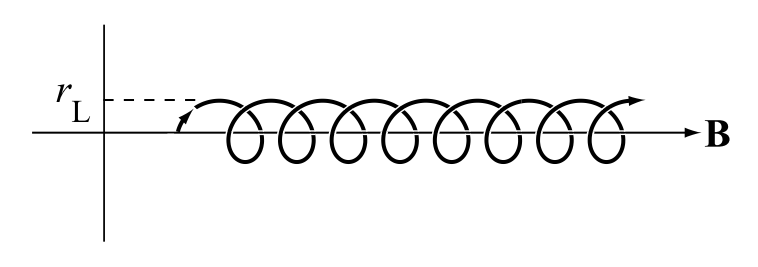
\includegraphics[width=0.525\textwidth]{Chp1/Helical_tray.png}
	\caption{  Helical trajectory of a charged particle in a uniform magnetic field ~\cite[Chapter~8]{Freidberg2007}.\label{Helical}}
\end{figure}

\section{Behind the plasma current}

Considering the drift of guiding center of a charged partice in a simple toroidal field in cylindrical coordinates $(R,\varphi,z)$. The component of the magnetic field $B_\varphi$ is the toroidal field and it decreases in the form of 1/R outward. The magnetic lines of force are circles around z axis. Particles in this  torus run fast in the toroidal direction and drift slowly in the $z$ direction as shown in figure~\ref{TDrift}, this drift is called toroidal drift. As a consequence  using only a toroidal component of magnetic field is not sufficient for confining the plasma inside a toroidal device or  tokamak  since particles drift and therefore will cause a loss of confinement ~\cite[Chapter~3]{Miyamoto2011}.\smallskip


\begin{figure}
	\centering
	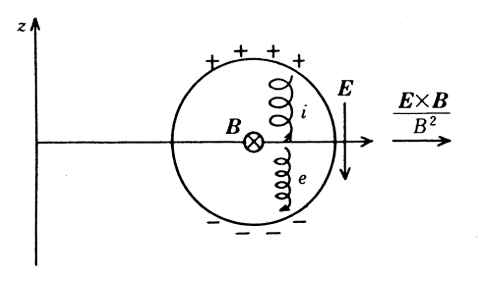
\includegraphics[width=0.55\textwidth]{Chp1/ToroidalDrift.png}
	\caption{Toroidal drift, particles drift in the vertical direction. ~\cite[Chapter~3]{Miyamoto2011} \label{TDrift}}
\end{figure}



If a current is induced in a toroidal plasma, the component of magnetic field around the magnetic axis (which is also called minor axis) is introduced. This component $B_P$ is called poloidal magnetic field and has components in $(R,z)$. The addition of this field creates magnetic lines circling the major axis of the torus, thus the particles circulate through the force lines. These lines cross a certain cross-section $P$ of the torus, each time the lines cross the plane $P$, the crossing point rotates around the minor axis by a certain angle $\iota$ which is called "rotational transform angle", this is shown in figure ~\ref{rot_angle}. The combination of toroidal and poloidal magnetic fields avoids the drift  described before originated by having an only-toroidal magnetic field by the introduction of the  rotational transform angle. The poloidal field in a tokamak is mainly produced by the induced plasma toroidal current.  \smallskip

\begin{figure}
	\centering
	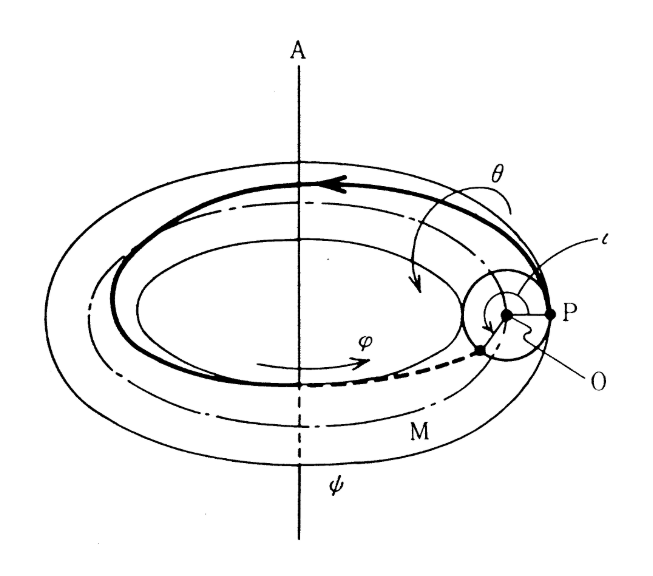
\includegraphics[width=0.655\textwidth]{Chp1/rotational_angle.png}
	\caption{Rotational transform angle $\iota$ formed when the magnetic force lines generated by the combination of toroidal and poloidal field cross the plane $P$ in different points  ~\cite[Chapter~3]{Miyamoto2011}. \label{rot_angle}}
\end{figure}

 All toroidally confined plasmas experience  outward toroidal forces along the $R$ direction, the first one is called the "hoop force" and is analogous to  the outward expansion force generated by the current flowing in a circular loop of wire, for this case this force corresponds to the toroidal current flowing in the plasma or simply called plasma current $I_p$. The second force is called "1/R force" and its name comes from the 1/R dependence of the toroidal field resulting from the toroidal geometry, the applied toroidal field $B_{\phi a}$,  where $a$ is the minor radius of the tokamak or the distance from the center of the vacuum chamber to the wall, has a 1/R dependence which follows from integrating Ampere's law around any closed toroidal loop located between the toroidal coils and the plasma. Finally the third one is called "tire tube force" and its existence is related to the difference of plasma pressures created by the toroidal geometry ~\cite[Chapter~11]{Freidberg2007}. \smallskip 
 
Given these outward toroidal forces, somehow the  toroidal force balance must be establish before the plasma hits the walls. An inwardly pointing restoring force is required and it is apply by means of the external poloidal field (PF) coils which generate a vertical field in order to compensate the radial forces generated by the tokamak.  By choosing the magnitude and sign of the vertical field correctly, one can produce an inward restoring force to produce toroidal force balance. In order to make an analytic deviation of the toroidal force balance a simple model for the magnetic fields is used, this model consists of a toroidal plasma whose contours of constant pressure are a set of nested concentric circles $p=p(r)$ , where $r$ is the minor radius coordinate as shown in figure~\ref{tor_geo}. The simplified version of the pressure and magnetic fields to be used in the determination of the toroidal force balance are:

	\begin{equation}
	\begin{aligned}
	p=&p(r)\\
	B =& \frac{R_0}{R}B_{\phi}(r) \hat{\phi} + \frac{R_0}{R}B_{\theta}(r)\hat{\theta}+B_v \hat{z}
	\end{aligned}
	\end{equation}
	
where $R_0$ is the tokamak major radius or the distance from the center of the torus to the center of the chamber (see figure ~\ref{tor_geo}), $B_{\theta}$ is the poloidal field and $B_v$ the external vertical field generated by the PF coils. After substituting the expression for the magnetic field into the general MHD force balance equation or the so-called Grad-Shafranov equation (~\cite[Chapter~6]{Miyamoto2011},~\cite[Chapter~11]{Freidberg2007},~\cite[Chpater~2]{Zohm2015}), the expression for the toroidal force balance can be obtained.
\smallskip

\begin{figure}
	\centering
	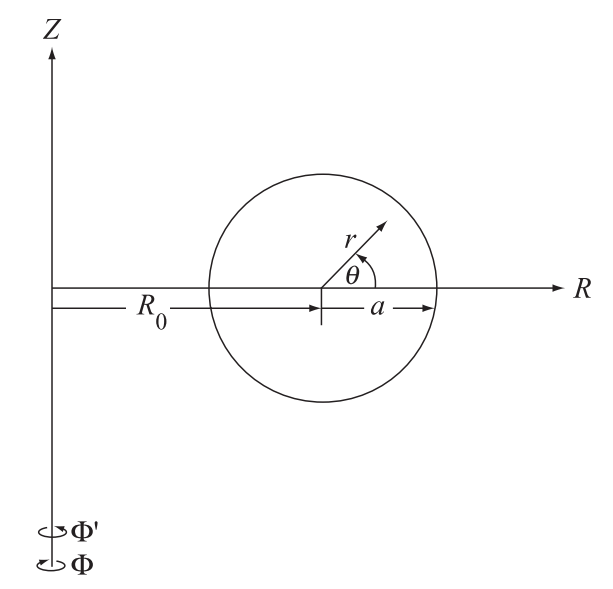
\includegraphics[width=0.6\textwidth]{Chp1/toroidal_geo.png}
	\caption{  Toroidal geometry and variables used for the calculations of the toroidal force balance and the vertical field~\cite[Chapter~11]{Freidberg2007}.\label{tor_geo}}
\end{figure}
%this is achieved by means of the application of an external vertical field.$


The toroidal force balance establishes the forces equation $F_{hoop}+ F_{1/R} + F_{tube}+ F_{v} =0$, where $F_v$ is the force generated by the external vertical field. Thus, the hoop force is given by:

\begin{equation}
F_{hoop}=2\pi^2a^2(li+le+2)~\frac{B_{\theta a}^2}{2\mu_0}
\end{equation}
 where $le$ and $li$ are the external and internal normalized inductances, $l= (L/2\pi R_0)/(\mu_0/4\pi)$. The "1/R" force is established as:
 
 \begin{equation}
 F_{1/R}=2\pi^2a^2 \left(\frac{ B_{\phi a}^2}{2\mu_0 }-\frac{\langle B_{\phi}^2 \rangle}{ 2\mu_0}\right)
 \end{equation}

where $\langle B_{\phi}^2 \rangle$ is the toroidal field average. The "tire tube" force is given by:
\begin{equation}
F_{tube}=2\pi^2a^2\langle p \rangle
\end{equation}

and finally the external vertical force is:

\begin{equation}
F_v=-2\pi^2a^2\left(\frac{2R_0 B_v B_{\theta a}}{a\mu_0}\right)
\end{equation}
 where $B_v$ is the external vertical magnetic field. Doing the combination of the 4 forces into the forces equation, the required vertical field for toroidal force balance remains:
 
 \begin{equation}
 B_v=B_{\theta a} ~\frac{a}{4R_0}\left[ \frac{2\mu_0 \langle p \rangle }{ B_{\theta a}^2} ~+~\frac{ B_{\phi a}^2 - \langle B_{\phi}^2 \rangle }{B_{\theta a}^2 } +li+le+2 \right]
 \label{force_balance}
 \end{equation}
  $B_v$ is the necessary vertical external field in order to avoid the plasma moving outwardly and touch the chamber walls, this equation will be addressed in chapter 4. In a purely vertical field, the plasma does not experience a vertical force and the vertical plasma current position is not well defined \cite[Chapter~4]{Zohm2015}. Due to the form  that the PF coils are positioned around the vessel the field produced by them is not completely vertical generating thus a radial component of  external magnetic field.  Due to Lorentz force law  the radial component of the external field  causes a vertical displacement of the plasma, this is compensated by adding another set of PF coils which generates an horizontal magnetic field. Figures ~\ref{PFcoils} show the field lines created by the vertical PF coils and its geometrical configuration surrounding the vacuum chamber. \smallskip
  
  \begin{figure}
  	\centering
  	\begin{subfigure}[b]{0.39\textwidth}
  		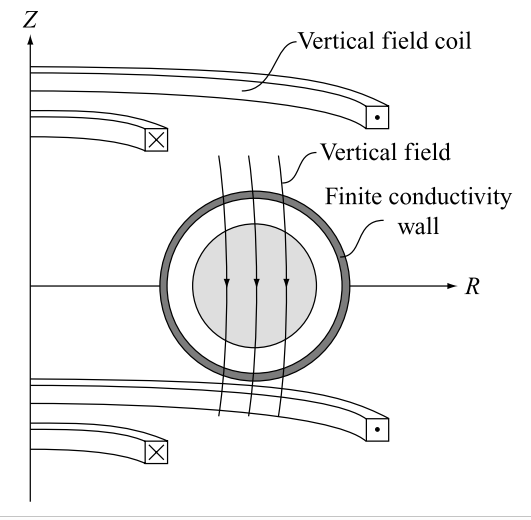
\includegraphics[width=\textwidth]{Chp1/PFcoils.png}
  		\caption{ Qualitative positioning of a set of vertical PF coils in a tokamak ~\cite[Chapter~11]{Freidberg2007}. The Pf coils depicted consist of a set of quadrupole coils, whit the internal coils currents in the opposite direction to one in the external coils. \label{} }
  	\end{subfigure}
  	~~
  	\begin{subfigure}[b]{0.39\textwidth}
  		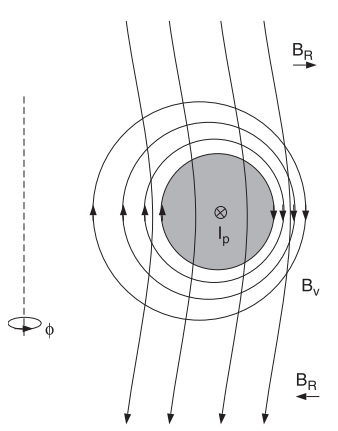
\includegraphics[width=\textwidth]{Chp1/horizontalField.png}
  		\caption{ Magnetic field lines created by the vertical PF coils with a radial field component as a result of the PF coils geometry \cite[Chapter~4]{Zohm2015}. \label{}    }
  	\end{subfigure}
  	\caption{ PF vertical coils and magnetic field lines.\label{PFcoils} }
  \end{figure}
  
  
  
\section{Plasma control in tokamaks}

Tokamaks are devices with an axisymmetric configuration with a large toroidal magnetic field and a DC toroidal current or plasma current $I_p$, given its physical characteristics and its performance until now is presently the leading candidate to become the world’s first fusion reactor. During the start up and subsequent approximately steady state phase of many fusion plasma discharges a toroidal current is induced in the plasma by means of transformer action with the plasma being the secondary of the transformer  ~\cite[Chapter~9]{Freidberg2007}. Sometimes the PF coils means both the equilibrium field coils and the ohmic heating coils. By raising the current of the primary windings of the current transformer (ohmic heating coils), a current is induced in the plasma, which acts as the secondary winding,for example at the ISTTOK tokamak the plasma is heated by the ohmic heating coils which also generate a vertical magnetic field ~\cite[Chapter~16]{Miyamoto2011}. \smallskip

Typical operation of a tokamak discharge starts with the establishment of a large, steady, toroidal, magnetic field\footnote{Tokamaks should have superconductive toroidal coils since they do not dissipate power in steady state and require only a small amount os cooling power~\cite[Chapter~5]{Freidberg2007}.}. Next, neutral gas is injected into the vacuum chamber and often pre-ionized. The transformer induced the plasma current $I_p$ which is then ramped up to its maximum value and maintained for the “flat top” portion of the pulse~\cite[Chapter~13]{Freidberg2007}. Since currently tokamaks have a plasma pulsed nature of some ~ms or ~s, in the case of bigger devices, it is easy to acquire a large volume of data over short periods and archived it after the plasma discharge or even during the plasma discharge, data acquisition and storage of signals in tokamaks is vitally important since the collected data us use for modeling the plasma, study instabilities and develop new codes and algorithms. \smallskip

Usually tokamak control tends to reefer to the control of the plasma itself, the supervisory plant control is conventional and normally uses industrial equipment. Control engineering for magnetic confined plasmas  embrace different types of techniques and they are use for  controlling the  physical variables existing on the device and the plasma. The tokamak control problems can be separated into two major classes: electromagnetic control and plasma kinetic control. Electromagnetic control refers to controlling the magnetic and electric fields and kinetic control refers to controlling particle feed rates and heating to modify the plasma density, temperature, pressure and current density \cite[Chapter~1]{PirontiBook}.  One of the main tasks of control engineering in the field of fusion is to maintain the plasma in certain position and shape in such way that it stays stable, follows set points and rejects possible instabilities which may occur maintaining a constant plasma current. \smallskip

Early tokamaks were quite primitive. The desired plasma parameters were obtained as a result of sets of pre-programmed power-supply or gas-valve commands, designed by trial and error. As technology tokamak began to develop and the plasma pulses duration became longer, feedback control loops were integrated to control simple parameters ~\cite{Lister1999}. It is natural that one of the first parameters to be actively controlled in a tokamak was the plasma position since this would mean maintaining the hot plasma centered inside the vacuum vessel. As already explained in last section coupling between the plasma radial position and current control systems depends on the active PF coil system. Initially, research efforts concentrated on the radial position control of circular, vertically stable tokamak plasmas \cite[Chapter~1]{PirontiBook}. By the end of the 1970's, the advantages of forcing the tokamak plasma cross-section to be other than circular  were being proposed on the basis of theoretical studies and the first plasmas with vertically elongated cross-sections were created. These elongated  plasmas are inherently unstable but this fact contributed to master the shape plasma control. \smallskip



\section{Thesis outline}

This thesis will study the properties and control applications for two tokamaks: JT60-SA and ISTTOK. These tokamaks possess physical characteristics which vary in big scale between them: the size, ISTTOK has a cross-circular section and JT60-SA is a diverted plasma, the dimension of the magnetic fields and plasma current, ISTTOK has 30 years operating and JT60-SA will start operations in late 2020, etc. Despite these facts there exist a big reason to join the two machines in a single work: both tokamaks rely on active magnetic control applied to the PF coils in order to control the plasma position and shape. Beyond  that, both use active magnetic control for the plasma position, also in this work for both tokamaks control and modeling approaches relying in the same concepts are applied.   \smallskip

This work is divided in 5 chapters being this chapter the Introduction.\smallskip

$\bullet$ Chapter 2 explores the plasma control systems implemented in different tokamaks around the world and addresses some important theoretical concepts to be applied in the further chapters.\smallskip

$\bullet$ Chapter 3 addresses JT60-SA operation, its theoretical modeling and assessments for the shape and plasma current control.\smallskip

$\bullet$ Chapter 4 presents the overall picture of ISTTOK tokamak: the geometry, the actuators and diagnostics. Following, the novel  implemented  reconstruction of the plasma current centroid position is addressed.\smallskip

$\bullet$ Chapter 5  presents the experimental control results in ISTTOK after the implementation of two different control algorithms in the device. \smallskip

The research done in this work is important and needed because it delves into topics crucial for tokamak operation. It asses control techniques for what will be the biggest operating tokamak (JT60-SA) and implements novelty algorithms in a small tokamak that probably would have not  existed on the ISTTOK tokamak without the latest technology advances. The main objectives of this thesis are to encompass the implementation of plasma position controllers for two different devices demonstrating that despite the size or characteristics of a tokamak it relies in the same physics principles and control engineering tools.\smallskip 


\chapter{Plasma  Control}
\label{Chap2}

This chapter summarizes some of the architectures for the Plasma Control Systems (PCS) existing in several tokamaks focused on the  Multi-threaded Application Real-Time executor (MARTe) framework.  The last part of this chapter addresses some basic concepts on state-space representation, linear dynamic systems and different feedback control techniques which will be widely used on the description of the carried out work showed on next chapters. 

\section{Overview of control systems}
The control of  plasma position, shape and current among other parameters is one of the essential engineering problems for present and future magnetic confinement devices. This chapter presents the real-time infrastructure used to implement plasma magnetic control and  some of the main reconstruction codes that are needed to achieve it. Real-time for fusion devices is principally focused on performing control and reconstruction algorithms, whether is for plasma position, current density, etc. on a software cycle, also known as sampling time, as short as possible so the  control loop acting on the  machine actuators can successfully take the plasma to the equilibrium, usually the real-time control cycles on some of the devices presented on this sections are on the order of  $\approx ~ 50~\mu s$ (\cite{Choi2018}, \cite{Felici2014} and ~\cite{Valcarcel2010}). The PCS deal with the overall control of  fusion devices being responsible also for the  plasma configuration and scenario algorithms \cite[Chapter~8]{PCS_2018}. Even thought this entire work mainly focuses on position and shape control it is also important to mention the relevance of density control for tokamak operation for the gas feeding feedback ~\cite{densityControl}. Industrial control systems in fusion devices like water cooling and power supply control usually are controlled outside the domain of the PCS. Currently different PCS's are used in  tokamaks around the world. In this chapter the "DIII-D-like" PCS, the Syst\'eme de Contr\^ole Distribu\'e (SCD) and MARTe will be introduced, this last one being of special interest due to its extensive utilization in this work, likewise this chapter presents an overview of the equilibrium codes  used for the reconstruction of plasma parameters used for the control of the  position, shape and plasma current among other parameters. The last part of this chapter recalls some basic concepts of Linear-Time Invariant systems and control system design which will be widely used in further chapters.


\subsection{DIII-D Plasma Control System}  

The DIII-D-like PCS is used in various fusion research facilities such as EAST (China), K-STAR (South Korea), NSTX (USA) and MAST (UK). Early documentation regarding the PCS in DIII-D\footnote{DIII-D is a D-shape tokamak operated by General Atomics in San Diego, California. } refers to digitalization of analog signals transmitted to a high speed processor executing a shape control algorithm and then writing the result to a digital to analog converter for driving the controlled systems. The real-time computer used allows to perform operations with vectors and matrices required for the plasma shape control algorithm \cite{DIIDcontrol}. Figure ~\ref{DIII1991} shows the block diagram of the DIII-D PCS 30 years ago.
\smallskip

\begin{figure}[htbp]
	\centering
	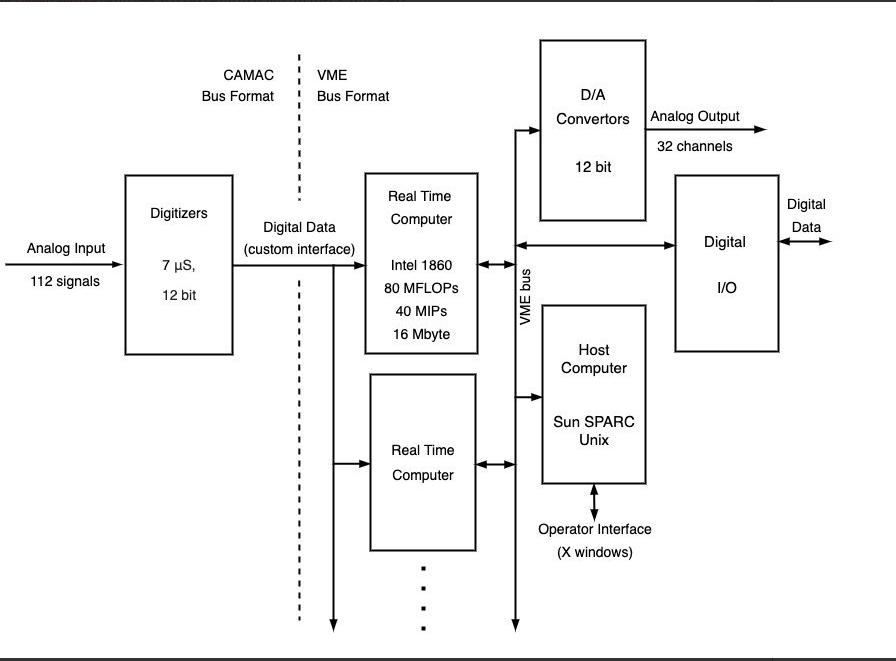
\includegraphics[width=0.65\textwidth]{Chp2/DIIDPCS_old.png}
	\caption{\label{DIII1991} DIII-D digital PCS in 1991 ~\cite{DIIDcontrol}.  }
\end{figure}

In recent years the DIII-D PCS had extensive software and hardware upgrades. The PCS present software consists of an infrastructure library core which provides all the routines that are necessary for implementing a basic and generic control system. The current  PCS hardware configuration uses a collection of  Intel Linux based multi-processor computers running in parallel to perform the real-time analysis and feedback control ~\cite{DIIID2013}. New digitalizers have been added to the real-time network to increase the number of signals acquired and to control hardware in real-time. Several real-time control algorithms were added and real-time data was added to external entities such as web server ~\cite{DIIIDnew}. In the current version of the PCS, a Myricom\footnote{Myricom networks also called Myrnet are high speed networking systems used to interconnect machines to form computer clusters. } network has been replaced with a 40 Gb/sec InfiniBand\footnote{InfiniBand is a network architecture from Mellanox designed to support I/O connectivity  and  reliability, availability, and serviceability Internet requirements ~\cite{MellanoxTechnologies2003}.  } network based on the Mellanox Connect-X 3\footnote{The Connect-X from the Mellanox company are Ethernet network interface cards with PCI Express.} hardware set. Figure ~\ref{DIIInew} shows the currently overall networking diagram of DIII-D PCS.


\begin{figure}[htbp]
	\centering
	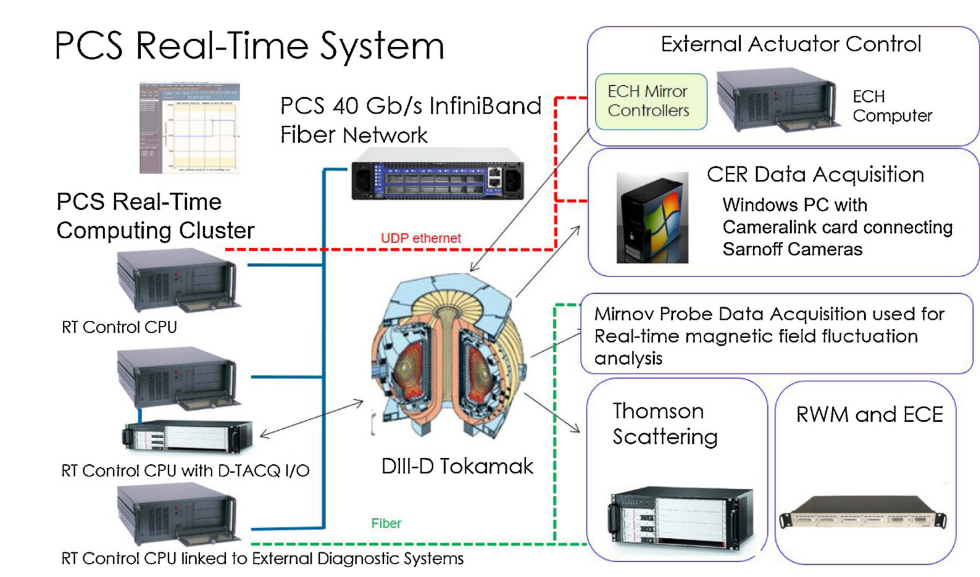
\includegraphics[width=0.65\textwidth]{Chp2/DIIIDPCSnew.PNG}
	\caption{\label{DIIInew} Actual DIII-D PCS real-time systems ~\cite{DIIIDnew}.  }
\end{figure}


\subsection{Syst\'eme de Contr\^ole Distribu\'e}

The TCV\footnote{The Tokamak \'a configuration variable (TCV) is  a medium size tokamak localized in Laussane,Switzerland. It is characterized by a highly elongated, rectangular vacuum vessel.} distributed control system uses a modular network of real time PC nodes linked by a real time network to provide feedback control over all of the actuator systems. Each node consists of a Linux PC either embedded on a Compact-PCI module or as a desktop computer with Intel CPU. A fiber optic ring network links the reflective memory (RFM) network cards in each node  \cite{TCVcntrl}.  The design of the diagnostic signal processing and control algorithms is performed in Matlab-Simulink software.  During the real-time execution  C/C++  code is generated from the Simulink and compiled  into a Linux shared library and distributed to target nodes  providing the input/output interface to the control algorithm code  ~\cite{TCVcntrl1}. Figure ~\ref{TCVcontrol} depicts the TCV SCD layout with the connectivity to diagnostics and actuators.


\begin{figure}[htbp]
	\centering
	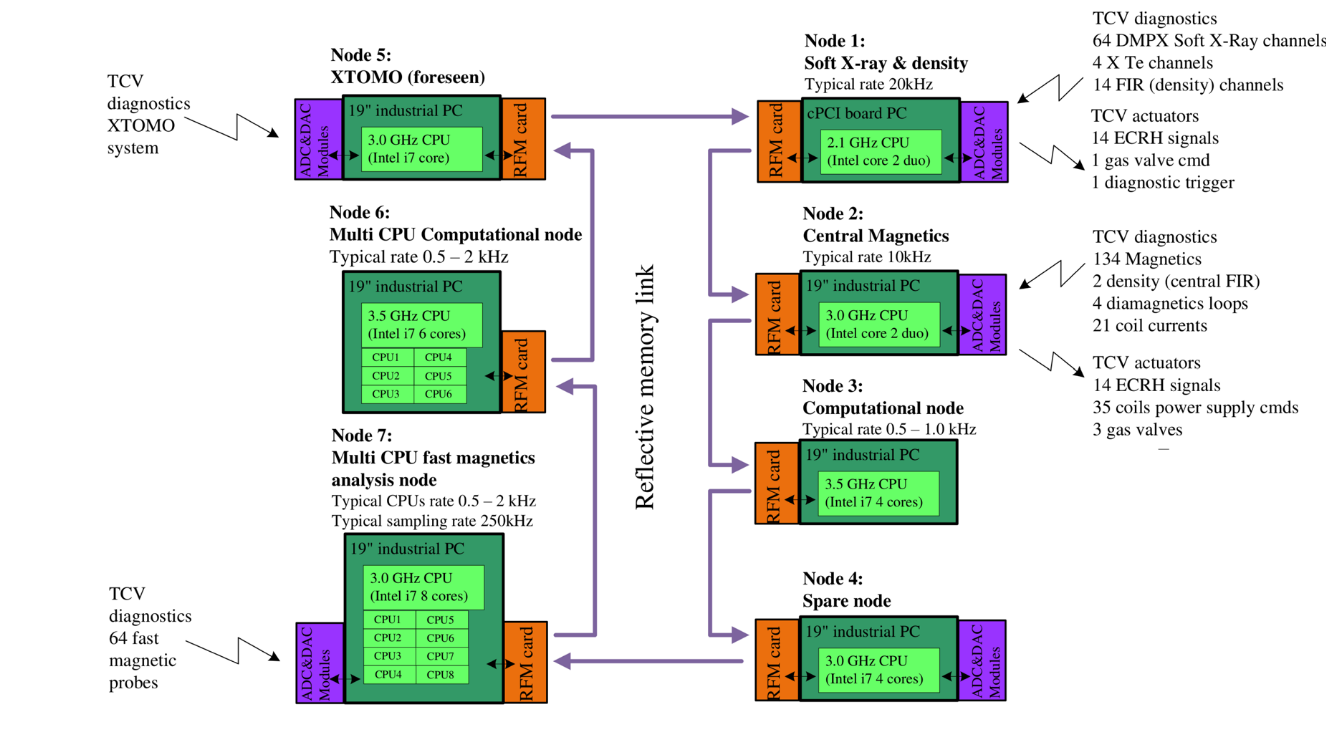
\includegraphics[width=0.65\textwidth]{Chp2/TCVcntrl1.png}
	\caption{\label{TCVcontrol} TCV SCD. Real-time network nodes connection. The nodes configurations 	are shown together with the typical diagnostic and actuator systems to which they are connected  ~\cite{TCVcntrl1}. This figure is missing the vertical stabilization controller that uses  Digital Signal Processors (DSP) system due to the higher control cycle speed of 5$~ \mu~s$ ~\cite{NunoPhD}. }
\end{figure}

\subsection{ASDEX Discharge Control System (DCS)}

The implemented control system existing on the ASDEX Upgrade  tokamak, the DCS  based on a modular software framework, supplies the functionality of  real-time diagnostic integration,  multivariable feedback schemes, actuator management,  monitoring and pulse supervision ~\cite{ASDEX2014}.\smallskip


 To distribute and parallelise the working load, part of the reconstructed  physical quantities are not computed by DCS but directly by real-time enabled digital diagnostic systems ~\cite{ASDEX2011}.  The DCS offers a user environment in the form of application processes (AP) holding the algorithmic part of control embedded in a framework infrastructure. Making use of the  polymorphic features of C++ the DCS  implements all infrastructure functions in base classes for the blocks, signals and other core component. The main components in DCS can be divided in function elements in the form of processes and DcsObjects, as well as data elements represented by signals, signal groups and parameters.  The hardware deployment of the DCS basically consists of a single-core 1 GHz PC with VxWorks operating system  and a multi-core 3.33 GHz PC running Concurrent Linux ~\cite{ASDEX2014}. Figure ~\ref{ASDEXcontrol} depicts the DCS control system function overview.  The blue boxes indicate the  sensor data sampling and measurement pre-processing, on magenta the control algorithms, the actuators on the red boxes and on the white boxes the references for the actuators and the segment scheduler which allows to select alternative sequences. 
 
 \begin{figure}[htbp]
 	\centering
 	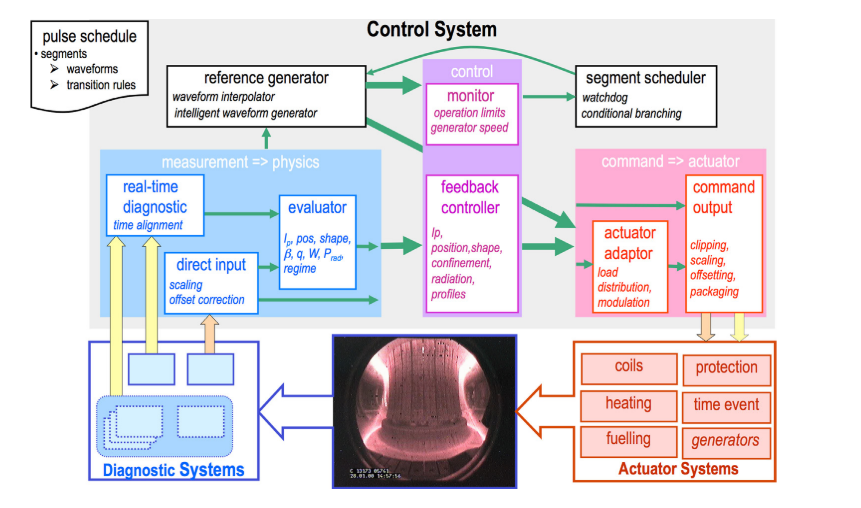
\includegraphics[width=0.75\textwidth]{Chp2/DCS_IPP.png}
 	\caption{DCS control system function overview. The blue boxes indicate the  sensor data sampling and measurement pre-processing, on magenta the control algorithms, the actuators on the red boxes and on the white boxes the references for the actuators and the segment scheduler which allows to select alternative sequences.   ~\cite{ASDEX2014}. \label{ASDEXcontrol}  }
 \end{figure}

\section{MARTe framework}

Regardless the nature of a real-time system, the design of it is usually related to the specific requirements it has, commonly this implies to have customized hardware and software which causes a lack in modularity and portability. When systems become bigger is convenient to provide a common library containing shareable functionalities and which also allows for modular implementations. In order to deal with this the MARTe framework was designed about a decade ago. MARTe was developed in order to standardize general real-time control systems for the execution of control algorithms and is based on a multiplatform $C^{++}$ library ~\cite{Neto2010},~\cite{JETRT}.  Previous implementations for a  software framework similar to MARTe were developed some years before for the JET tokamak. JETRT was a software framework used to develop real-time control and data acquisition systems which laid the foundation for current MARTe framework ~\cite{JETRT}. MARTe is currently used in several tokamaks such as JET, FTU, COMPASS and ISTTOK. 

  


\subsection{MARTe architecture }
The unitary MARTe component is the Generic Application Module (GAM). Each of the C++ programmed GAMs usually performs an specific task of the control system. The collection of interconnecting GAMs builds MARTe  \cite{Neto2011}. The GAMs  have an entry point to receive data driven configuration and a set of input and output channels to interface with other GAMs. The Dynamic Data Buffer (DDB) is a generic memory data bus where each GAM receives and produces data using DDB named channels. Usually each GAM is associated with a special function of the system like processing data of a specific diagnostic or perform some  control algorithm. MARTe hardware data interface and synchronization for inputs and outputs is performed using a special GAM called IOGAM. Figure ~\ref{GAMs} shows and xample of a set of GAMs connected to the DDB. Timing and hardware GAMs provide the I/O interface to the exterior, whereas a generic waveform GAM inputs the reference for a PID controller. Finally, the output is sent to a DAC and the data is stored for analysis by a collection GAM.  It should be noticed that the reference generation and the controller GAM are not aware of the changes in the data providers and data consumers.


\begin{figure}[htbp]
	\centering
	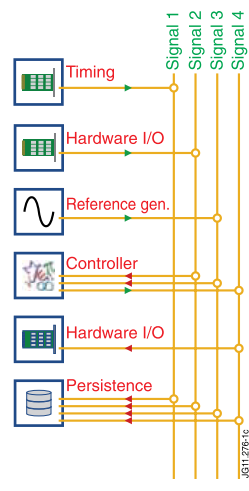
\includegraphics[width=0.35\textwidth]{Chp2/GAMs.png}
	\caption{\label{GAMs} MARTe GAMs structure using the DDB to exchange data in real-time.  \cite{MARTe2011}}
	
\end{figure}

\subsection{MARTe hardware containers}

This section describes the  hardware in-house developed at Instituto de Plasmas e Fus\~ao Nuclear (IPFN) for the use with the MARTe framework for the overall plasma control in different devices, specially the case for the JET, COMPASS and ISTTOK tokamaks. The devices presented in this thesis and used with the MARTe framework base their hardware on the  Advanced Telecommunications Computing Architecture (ATCA) standard, which is the most promising architecture to substantially enhance the performance and capability of existing standard systems as it is designed to handle tasks such as event building, feature extraction and high-level trigger processing ~\cite{ATCA2010}.\smallskip

At JET the data acquisition system for the vertical stabilization control is based on the PICMG 3.0 ATCA standard  and contains six data acquisition cards. Each board comprises 32 18-bit resolution analog-to-digital converters (ADC) acquiring at 2 Msamples/s. The cards are connected to the controller computer using the Peripheral Component Interconnect Express (PCIe) point-to-point links through the ATCA backplane ~\cite{Neto2010},~\cite{ATCA2006}. Data synchronization is performed in the master board, which is guaranteed by the firmware to be the latest to have data available. Once new data is available, it is collected and a new MARTe cycle starts. The CPU core isolation scheme allows to protect the real-time environment from spurious and undesired interrupt sources. Figure ~\ref{ATCa_JET} depicts a roughly JET scheme of the acquisition boards and its connection to the MARTe framework. The acquisition boards map in the controller computer memory a set of four buffers, the selected one is consecutively cycled every $50~ \mu s$  by the firmware. The first value written is the header and contains the absolute time since the last trigger, followed by the acquired  values of the ADCs, and finally by the footer containing the same value as the header. \smallskip

\begin{figure}[htbp]
	\centering
	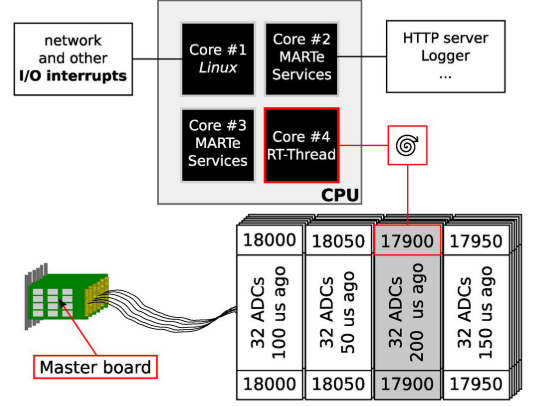
\includegraphics[width=0.55\textwidth]{Chp2/ATCA_JET.png}
	\caption{\label{ATCa_JET}  JET acquisition boards from the ATCA hardware  and its connection to the MARTe framework.  ~\cite{Neto2010}}
	
\end{figure}



The hardware used in the ISTTOK real-time control system is also  based on the ATCA standard while the old architecture was based on the Peripheral Component Interconnect (PCI) standard. It is worth to mention that the MARTe control cycle in ISTTOK is programmed to be of 100 $\mu s$, this value was calculated taking into account the time that each GAM takes to run. The ATCA acquisition boards are composed by 32  ADC modules connected to a Virtex-4 Field-programmable gate array (FPGA) that manages the data path from the ADC to the PCIe bus.  Since ISTTOK has a noisy environment and the selected ADCs were able to acquire data at 2 Msample/s, it was decided to implement an additional digital filter in the FPGA to filter each ADC sample with a finite impulse response (FIR) filter ~\cite{ISTTOK_RT}. Figure ~\ref{PCIe} shows a photograph of an ATCA board, each board contains 512 MBytes of DDR memory and an FPGA, which performs digital signal processing and includes a PCI Express communications interface. These hardware modules are developed at the IPFN where the ISTTOK tokamak is also located. Figure ~\ref{Tomog} shows a schematic example of how a tomography system installed at ISTTOK is connected to the ATCA boards.  \smallskip 

\begin{figure}[htbp]
	\centering
	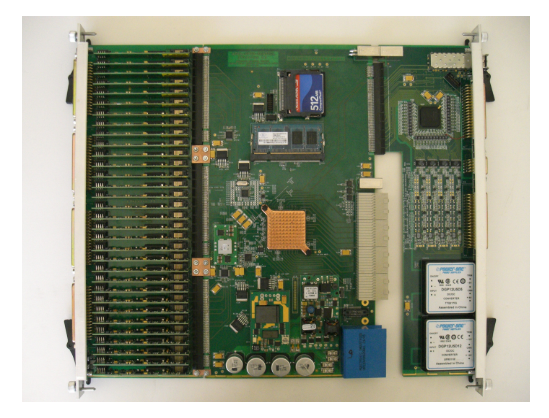
\includegraphics[width=0.5\textwidth]{Chp2/PCIboard.png}
	\caption{\label{PCIe}  ATCA control board with 32 ADCs developed and assembled  at the IPFN. \cite{ATCA2010}}
	
\end{figure}

\begin{figure}[htbp]
	\centering
	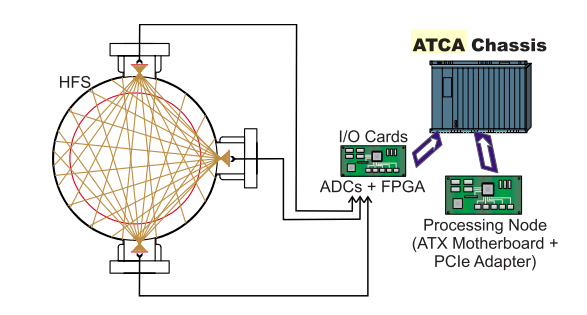
\includegraphics[width=0.55\textwidth]{Chp2/Tomogr.png}
	\caption{\label{Tomog}  The ISTTOK tomography system has 30 acquisition channels connected by an Input-Output ATCA card and processed using the MARTe framework.  \cite{Ivo_tomo}}
	
\end{figure}

For the Compass Tokamak ( Prague, Czech Republic), its whole control and data acquisition system was redesigned and built from scratch, based also on the ATCA standard. In total 14 ATCA  boards (developed at IPFN) will be used with 32 ADCs each one. In order to guarantee real-time execution of the control codes a framework based on Linux and the Real-Time Application Interface (RTAI) will be used. This will explore the features provided by the new multi-core technologies \cite{ATCA2010}. Figure  ~\ref{Compass} shows an schematic of the new COMPASS system.
\smallskip


\begin{figure}[htbp]
	\centering
	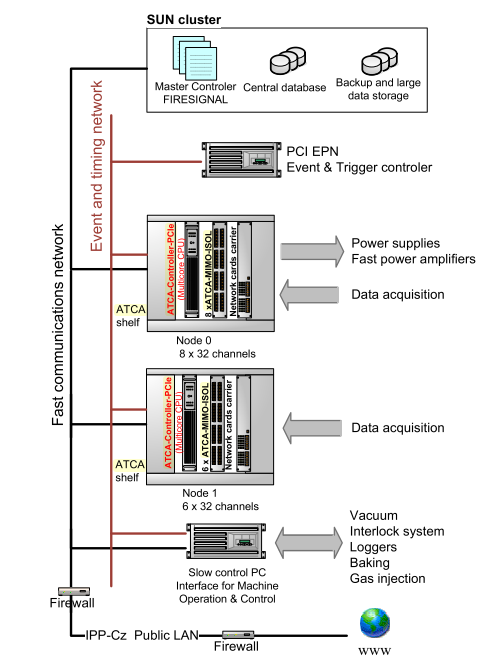
\includegraphics[width=0.55\textwidth]{Chp2/COMPASS_ATCA.png}
	\caption{\label{Compass} Schematic of COMPASS tokamak control and data acquisition
		system,  two ATCA systems are responsible for the fast control of the device and for the data acquisition. \cite{ATCA2010}}
	
\end{figure}

\subsection{MARTe 2.0}
Software Quality Assurance (QA)\footnote{Software QA is a set of activities or processes that define and assess the adequacy of software processes to provide evidence that establishes confidence that the software processes are appropriate for and produce software products of suitable quality for their intended purposes~\cite[Chapter 5.1]{SQA}.} processes are being applied to the development of a new version of the MARTe framework also  called MARTe 2.0. The  main objective is to provide a QA certifiable environment from where it is possible to develop, with less effort, certifiable applications. The  MARTe QA version can be easily adapted to the development of many types of software which are common in the fusion community, in particular for software related to control and data acquisition systems that is to be shared among different teams  ~\cite{MARTe2}. MARTe 2.0 will be the result of reduction exercise of the core framework based on the lessons learned from MARTe. This version will incorporate and implement an integral quality assurance process for the development of the framework (e.g. unit tests and coding standard) ~\cite{MARTe2PMP}. 
\smallskip

In order to develop robust code and to avoid common errors and pitfalls, a controlled subset of the C++ language must be defined for the MARTe framework. This subset will be defined by means of a list of coding rules, which will address all dangerous aspects of the C++ language for critical systems. Thus, the C++ version used on MARTe will be defined by the standard ISO/IEC 14882:2003 aka as C++03, while the coding rules will be those defined by the standard MISRA C++:2008 ~\cite{MARTe2Code}. The MARTe project manager is responsible for appointing a quality office (QO) for the QA process. The QO will guarantee that the QA activities are executed accordingly to the software development process, it will also conduct independent reviews and audit all data and processes involving the development, production and maintenance of MARTe deliverables ~\cite{MARTe2QAP}. The overall advantage of the new MARTe version is that the common faced difficulties of distributing and maintaining a software without  the continuous support of the original developers will be overcome following a complete QA system.



\section{Plasma equilibrium codes} 

Tokamak equilibrium codes are used for retrieving information about plasma current, shape and position and pressures profiles among other parameters. Usually these codes use as input data as the machine geometry, the PF coils currents and the flux and magnetic field diagnostics measurements. The importance of these codes is that since some of the parameters necessary for an accurate feedback control are not directly measured from the diagnostics,  this data has to be fitted on real-time somehow to the Grad-Shafranov equilibrium model~\cite{Shafranov1971}. In this section some of the most implemented and reported codes for tokamak plasma equilibrium reconstruction will be briefly  described.
\smallskip 


The EFIT (Equilibrium Fitting) code is used to efficiently reconstruct the current profile parameters, the plasma shape  and a current density profile satisfying the MHD equilibrium constraint  based on a Picard iteration\footnote{Picard iterations is a method based on  successive approximations to obtain a set of conditions under which an initial value problem has a unique solution.} approach which approximately conserves the external magnetic measurements ~\cite{EFIT1985}. EFIT has served as the de-facto standard technique to infer equilibrium from experimental diagnostics and there have been many different code implementations of this technique, all EFIT versions  are able to solve the MHD force balance and most experiment-specific customizations are made for the addition of experimental constraints peculiar to the experiment being modelled~\cite{EFIT2013}. EFIT reconstruction code is used in tokamaks such as DIII-D and the National Spherical Torus Experiment (NSTX). For the specific NSTX case they implemented a special real-time EFIT version called rtEFIT developed at General Atomics, the rtEFIT code provides the shape of the plasma boundary that is used as input to an isoflux control algorithm that generates voltage requests to the power supplies. The reconstruction of plasma boundaries  in real-time compare well to those reconstructed using the EFIT code offline in between plasma discharges ~\cite{rtEFIT}.
\smallskip


The RAPTOR (RApid Plasma Transport simulatOR)  is a model-based control-oriented code that predicts tokamak plasma profile evolution in real-time, it predicts the evolutions of several parameters, thanks to its accurate yet simplified physics model \cite{Raptor}. The physical model of the plant is derived from a spatially discretized partial differential equation (PDE), yielding a nonlinear set of ordinary differential equations (ODEs) for which the derivatives are evaluated analytically by the RAPTOR code. One of the main RAPTOR features is that  while the plasma is evolving RAPTOR has full knowledge of the plasma profiles and the available real-time diagnostic data can be included in a natural way to improve the accuracy of the estimation, in control engineering this approach is known as dynamic state observer and is used to estimate unmeasured or  poorly states of a dynamical system ~\cite{RAPTOR2011}. This dynamic state observer consists on an extended Kalman filter which estimates an augmented state consisting of physical states and random-walk disturbances  ~\cite{RAPTOR2014}. The concepts of  states-space systems and Kalman filtering will be addressed in the next subsections.  Figure ~\ref{RaptorMARTe} scheme shows  the  integration of the RAPTOR code on top of the MARTe framework at the Italian tokamak RFX-mod.
\smallskip

\begin{figure}[htbp]
	\centering
	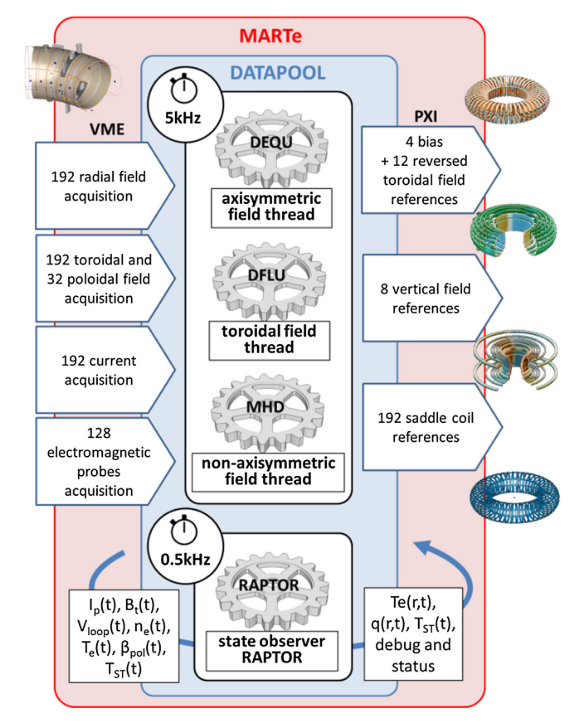
\includegraphics[width=0.505\textwidth]{Chp2/raptorMARTe.png}
	\caption{\label{RaptorMARTe} Skectch of the integration of the state observer RAPTOR in the RFX-mod real-time control system based on the MARTe framework.
		experimental \cite{Raptor}}
	
\end{figure}

For the case of JET  a  boundary reconstruction package called XLOC has been used to identify the X-point position and plasma boundary ~\cite{xloc}.  A newer code relying on XLOC  called Equinox was designed and implemented in C++ using a finite element method and a non linear fixed point algorithm associated to a least  square optimization procedure to reconstruct the plasma equilibrium in less than 50ms for the real-system~\cite{equinox}. 
\smallskip


The CREATE  codes (CREATE-L~\cite{Albanese:CREATEL} and CREATE-NL~\cite{Albanese:CREATENL}) are  equilibrium solvers which are widely described in next chapter as well as their application to plasma shape and position control design for the JT-60SA tokamak.
 


\section{Control Techniques and State-Space models}

This section will summarize  some systems dynamics and control  concepts which will be applied on the next chapters.\smallskip

 Applying a feedback control loop to a system  brings a link between the output and input signals, this action corrects the error in between the system output and a desired set-point,  eventually  the objective  of any closed loop controller is to take and maintain  the output signal at a prescribed value. The reduction of the system error is merely one of the many important effects that feedback may have upon a system, that is the reason why this sections will deepen in several control techniques ~\cite[Chapter~1]{Golnaraghi2010}. This section will also delve into the state-space models concepts since it will be a recurrent representation  for several systems presented in next chapters.

\smallskip

\subsection{State-Space models}
\label{SS_subsec}
State-space models are  crucial for the overall development of the work presented on this thesis whether they are used to describe a tokamak linear model for plasma position and  shape control or used to model some other relevant variables.  The first concepts  to be summarized on this section are the state variable and state equation definitions (\cite[Chapter~10]{Golnaraghi2010}, ~\cite[Chapter~2]{Kailath1980}).   \smallskip

Let the $n$ state equations of $nth$-order dynamic system be represented as:

\begin{equation}
	\frac{dx_i (t)}{dt} ~ = ~ f_i [x_1(t),x_2(t),...,x_n(t), u_1(t),u_2(t),...,u_p(t),w_1(t)w_2(t),...,w_v(t)]
	\label{stateEqs}
\end{equation}

 where $i=1,2,..,n$. The $ith$ state variable is represented by $x_i(t)$; $u_j(t)$ denotes the $jth$ input for $j=1,2,..,p$; and $w_k(t)$ denotes the $kth$ disturbance\footnote{The unknown disturbances acting on the state-space model are assumed to be generated by independent stochastic noise vectors. } input, with $k=1,2,..,v~$.\smallskip
 
 Let $y_1(t),y_2(t),...,y_q(t) $ be the q system output variables. The output variables are functions of the state variables  and the input variables. The output equations can be expressed as:
 \begin{equation}
 	y_j(t)=g_j[x_1(t),x_2(t),...,x_n(t),u_1(t),u_2(t),..,u_p(t),w_1(t)w_2(t),...,w_v(t)]
 \label{outputEq}
 \end{equation}
 
 where $j=1,2,..,q$~.
 \smallskip
 
 The set of $n$ state equations from ~\ref{stateEqs} and the $q$ output equations in ~\ref{outputEq} together they form the \textit{dynamic equations}. In order to have an easier form of expression and manipulations of these equations is common to represent them in vectors and matrices as follows: \smallskip
 
 \textbf{State vector:}
 \begin{equation}
 x(t)=
 \left[
 	\begin{matrix}
 	x_1(t)\\
 	x_2(t)\\
 	\vdots\\
 	x_n(t)
 	\end{matrix}
 	\right] 
 \end{equation}
 
\textbf{ Input vector:}
 
  \begin{equation}
 u(t)=
 \left[
 \begin{matrix}
 u_1(t)\\
 u_2(t)\\
 \vdots\\
 u_p(t)
 \end{matrix}
 \right] 
 \end{equation}
 
 \textbf{ Output vector:}
 
   \begin{equation}
y(t)=
 \left[
 \begin{matrix}
 y_1(t)\\
 y_2(t)\\
 \vdots\\
 y_q(t)
 \end{matrix}
 \right] 
 \end{equation}
 
\textbf{ Disturbance vector:}
    \begin{equation}
 w(t)=
 \left[
 \begin{matrix}
 w_1(t)\\
 w_2(t)\\
 \vdots\\
 w_v(t)
 \end{matrix}
 \right] 
 \end{equation}
 
 Using these defined vectors, equation ~\ref{stateEqs} can be written for the $n$ states like:\smallskip
 
 \begin{equation}
 	\frac{dx(t)}{dt}~=~ f[x(t),u(t),w(t)]
 \end{equation} 
 where f is a vector containing the functions $f_1,f_2,..,f_n$ as elements. In the same way the equations from ~\ref{outputEq} become:
 \begin{equation}
 	y(t)=g[x(t),u(t),w(t)]
 \end{equation}
 where $g$ is a vector containing the functions $g_1,g_2,..,g_n$ as elements.
 
 For a system that is time-invariant and linear like the ones shown on next chapter, the equations can be re-writen as:
 
 \begin{align}
	\frac{dx(t)}{dt}~=~ Ax(t)~+~Bu(t)~+Ew(t) \\
	y(t)=Cx(t)+Du(t)+Hw(t)
 \end{align}

  where $A$ is the state matrix, $B$ is the input matrix, $C$ is the output matrix, $D$ is the feed-forward matrix and  $E$ and $H$ are disturbances matrices. For simplification is usual the study of state-space and controllers concepts under the assumption that $w(t) =0$ which leads to the form:
 \smallskip
 \begin{align}
 	 \frac{dx(t)}{dt}~=~ Ax(t)~+~Bu(t)\\
 	  y(t)=Cx(t)+Du(t)
 	  \label{SS_eqs}
 \end{align}

 When applying the Laplace transform to system from ~\ref{SS_eqs} it leads to:
 \begin{align}
 	x(s)=(sI-A)^{-1}[x(0)+Bu(s)]\\
 	y(s)=C(sI-A)^{-1}[x(0)+Bu(s)]+Du(s)
 	\label{SS_eqs_lap}
 \end{align}
 
 where $x(0) $is the initial state or initial conditions from the system~\cite[Chapter ~4]{Chen1999}. The representation of the system from equation ~\ref{SS_eqs_lap} will be used in next subsections.\smallskip
 
State-space dynamics can describe Multiple-Input Multiple-Output (MIMO) models where a number of inputs $n_{~inputs}>~1$ can relate through the dynamics  matrices of the system to a number of outputs $n_{~outputs}>~1$. Given the physical conditions of the systems that will be analyzed and controlled in this work MIMO models will show several times.


\subsection{PID control}
\label{PID_sec}
This subsection will shortly address the Proportional-Integral-Derivative (PID) control  concepts. PID controllers are presently the most common ones in industrial applications and they are used several times through all this work. The PID controller has three parameters; proportional gain, integral gain, and derivative gain, they have proved through the years to provide a suitable control for a variety of systems despite not being optimal always. The usefulness of PID controls lies in their general applicability to most control systems. In particular, when the mathematical model of the plant is not known and therefore analytical design methods cannot be used, PID controls prove to be most useful.  
\smallskip

The closed-loop systems compensate the disturbances by measuring the output
response, feeding that measurement back through a feedback path, and comparing
that response to a reference or set point. If there is any difference between
the two signals, the system drives the plant, via the actuating signal, to make a
correction. If there is no difference, the system does not drive the plant, since the
plant’s response is already the desired set point ~\cite[Chapter ~1]{Nise}. Closed-loop systems also focus on achieving the stability as a system must be stable in order to produce the proper transient and steady-state response~\cite[Chapter ~3]{Nise}, thus if the closed-loop system poles are in the left half of the plane the feed-back system will be stable.
\smallskip

Systems that feed the error forward to the plant are called proportional control systems. Systems that feed the integral of the error to the plant are called integral control systems. Finally, systems that feed the derivative of the error to the plant are called derivative control systems~\cite[Chapter ~9]{Nise}. A PID controller consists on a feedback control loop where the current, previous and future error signal  between the output of the system and a given set point, is multiplied by the PID gains  and then sumed converting this signal into the system input, the effects on the feedback loop from each one of the gains will be described.

 When the model of the system plant is known it is possible to apply designing techniques for the PID gains like the Ziegler-Nichols method. When is not the case analytical or even intuition arising from the physics and numerics of the problem should be applied. Figure ~\ref{PID_scheme} shows the block scheme of a PID controller with a system plant $G(s)$ on the Laplace domain.

\begin{figure}[h]
	\centering
	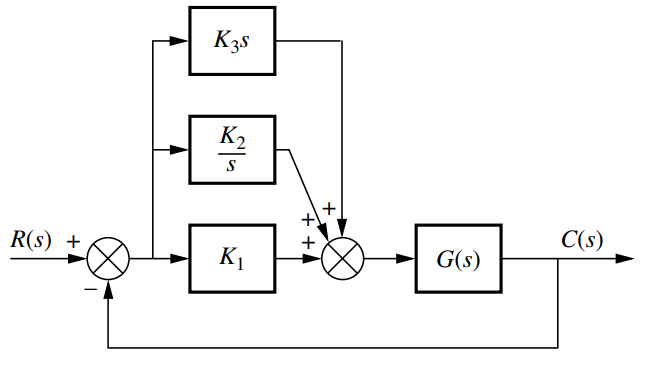
\includegraphics[width=0.55\textwidth]{Chp2/PID_scheme.png}
	\caption{ Plant and PID controller block scheme on Laplace domain ~\cite[Chapter~ 9]{Nise}. \label{PID_scheme}}
\end{figure}

 An only  proportional controller   relates the output of the system to the input by a proportional constant, and even though it performs a first approach to follow the  set point and stabilizes,  it results in a steady-state error or offset, such error may be eliminated with integral control action, see figure ~\ref{propGain}.
\smallskip

\begin{figure}[h]
	\centering
		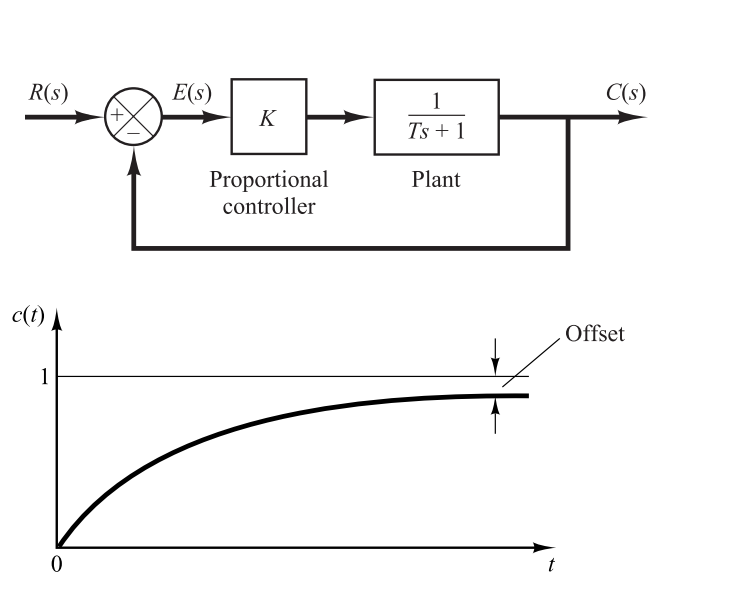
\includegraphics[width=0.55\textwidth]{Chp2/propgain.png}
	\caption{ Plant with a proportional (P) control  scheme on the Laplace domain and its response to a unit-step. The offset or error between the steady-sate response is also pointed out~\cite[Chapter~ 5]{Ogata2009}. \label{propGain}}
\end{figure}


The integral gain produces a signal that is proportional to the time integral of the error system, the offset or steady-state error can be eliminated by the sum of an integral action, the integral term also tends to produce and oscillatory response. This is an  important improvement over the proportional control alone, which gives an offset. Since the PI controller is also a low-pass filter, it helps filtering out the high-frequency noise  ~\cite[Chapter ~9]{Golnaraghi2010}, ~\cite[Chapter~ 5]{Ogata2009}. Figure ~\ref{PI} shows the block scheme of a PI controller and its response to a unitary step.
\smallskip

\begin{figure}[h]
	\centering
	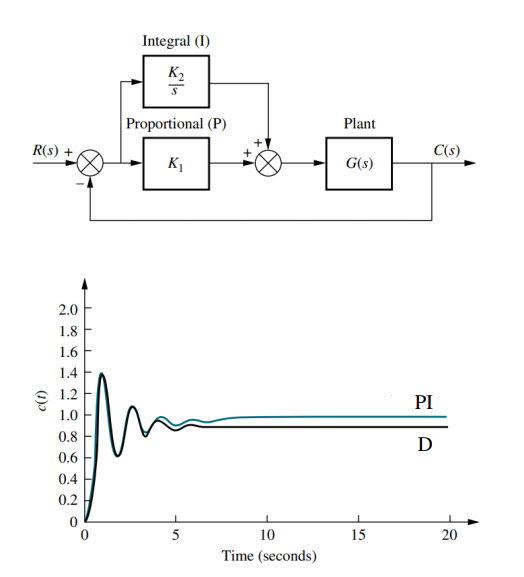
\includegraphics[width=0.55\textwidth]{Chp2/PI_Dcomp.png}
	\caption{  Plant scheme of   a plant with  a proportional-integral (PI) control   on the Laplace domain. Bottom graph corresponds to a step response to closed-loop systems with D and a PI controller ~\cite[Chapter~ 9]{Nise}, a visible improvement on the state-state error with the PI control is observable.  \label{PI}}
\end{figure}

The derivative gain added to a proportional controller gives a more sensitive controller which responds to the rate of change of the error and can produce a significant correction before the magnitude of the error becomes to large. In general, derivative control anticipates the actuating error, adds damping  and tends to increase the system stability, figure~\ref{propderGain} depicts the scheme and system response with a PD controller. The PD control uses the error derivative ~$de(t)/dt$ which allows the control to anticipate the error direction, it initiates an early corrective action which means an improvement on the transient response   ~\cite[Chapter ~9]{Golnaraghi2010},~\cite[Chapter ~9]{Nise}. Normally in linear systems when the slope of $e(t)$ is large overshoots may occur, when using a PD controller it also corrects the overshoot. 
\smallskip

\begin{figure}[h]
	\centering
	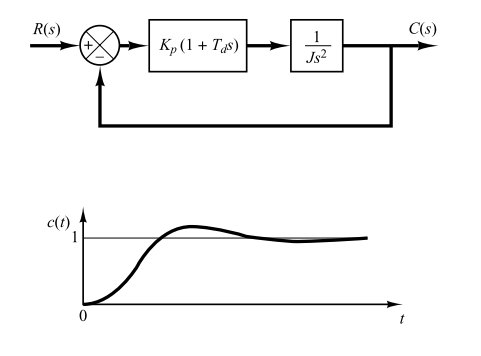
\includegraphics[width=0.55\textwidth]{Chp2/propderivgain.png}
	\caption{ The top scheme shows a PD controller for a  plant that is only modeled as an inertial load, on the graph below is shown the system response where it is possible to observe an offset reduction and a controlled transient as compared with the P controller ~\cite[Chapter~ 5]{Ogata2009}. \label{propderGain}}
\end{figure}

A PID controller improves the steady-state error and the transient response. Figure ~\ref{PID} shows the response time traces  of the same system with a PID, PD and D controllers to a unit step.
\smallskip



\begin{figure}[h]
	\centering
	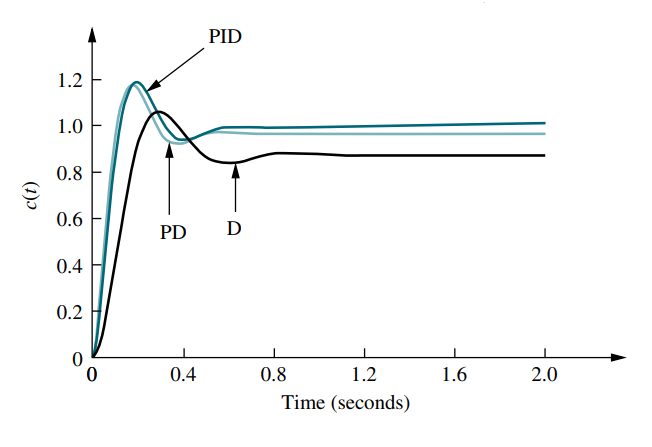
\includegraphics[width=0.505\textwidth]{Chp2/PID_comp.png}
	\caption{ Step response to closed-loop systems with D, PD and PID controllers ~\cite[Chapter~ 9]{Nise}. \label{PID}}
\end{figure}

\subsection{Multiple-Input Multiple-Output control}
\label{MIMO_sec}
This subsection will discuss the pole-place method and the linear quadratic optimal regulator (LQR) for control systems in state-space already discussed in subsection~\ref{SS_subsec}.  State feedback controllers basically relocate the eigenvalues of the given system through a state-feedback multiplication by a constant gain matrix $K$ so the system can follow a reference and be stabilized if necessary.
 \smallskip
 
 The concept of pole should be introduced as it will be related to  the definitions of the MIMO control methods. The poles $p_i$ of state-space system are the eigenvalues $\lambda_i(A),~i=1,..,n$ of the system matrix $A$. Poles are important for establishing the stability of a system, for continuous systems a linear dynamic system  $	\dot{x}(t)~=Ax(t)+Bu(t)$ , where $\dot{x}(t)$ stands for $dx/dt$, is stable if and only if all poles are in the open left half plane (LHP), that is $\mathbb{R}e~{\lambda_i(A)}<~0, \forall i$. Eigenvalues in the right half plane(RHP) with  $\mathbb{R}e~{\lambda_i(A)}\geq~0$ give raise to unstable modes since for this case $e^{\lambda_i(A)~t}$ is unbounded as $t\rightarrow~\infty$,  eigenvalues in the open LHP give raise to stable modes where $\mathbb{R}e~{\lambda_i(A)} \rightarrow 0$ as $t\rightarrow~\infty$~\cite[Chapter~4]{Skogestad}.
\smallskip

Consider the system:
\begin{align} 
	\dot{x}(t)~=Ax(t)+Bu(t) 	\label{SS_eq}\\
y(t)=Cx(t) \nonumber
\end{align}

where it is assumed that $D=0$. In state feedback, the input $u(t)$ is given by:

\begin{equation}
	u(t)=r(t)-Kx(t) = r(t)-[k_1~ k_2~\cdots ~k_n] x(t)=r-\sum_{i=1}^{n}~k_ix_i
	\label{u(t)}
\end{equation}

as shown in figure~\ref{SS_schm}. Each feedback gain $k_i$ is a real constant.This is called the constant gain negative state feedback or in a simpler form \textit{state feedback}~\cite{Chen1999}. Substituting equation ~\ref{SS_eq} into ~\ref{u(t)} its obtained:
\begin{align} 
\dot{x}(t)~=(A-B~K)x(t)+Br(t) \label{SS_eq_feed} \\
y(t)=Cx(t) \nonumber
\end{align}



\begin{figure}[h]
	\centering
	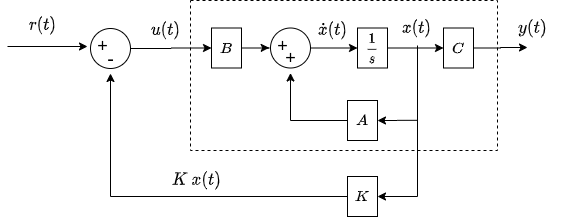
\includegraphics[width=0.6\textwidth]{Chp2/SS_scheme.png}
	\caption{  State-space model with a $K$ gain matrix feedback scheme.\label{SS_schm}}
\end{figure}


The first control MIMO algorithm to be addressed  is the pole-placement method which consists in placing the closed-loop system poles in certain location by means of state feedback through an appropriate state feedback gain matrix $K$, the design objective of the pole-placement design is to find  $K$ such that the eigenvalues or poles of $(A-BK)$, or the closed-loop system, are of certain prescribed values. For this method the eigenvalues of the closed-loop system can be assigned arbitrarily  as long as they are stable~\cite[Chapter~10]{Golnaraghi2010}. The  determination of the desired closed-loop poles is based on the transient-response and/or frequency-response requirements, such as speed, damping ratio, or bandwidth, as well as steady-state requirements ~\cite[Chapter~10]{Ogata2009}.
\smallskip

Let's consider the system given in equation ~\ref{SS_eq_feed} and the feedback control input from ~\ref{u(t)}, by substituting one on the other the closed-loop system is represented by the equation:
\begin{equation}
	\dot{x}(t)=(A-BK)x(t) + Br(t)	\quad ,
\end{equation}

 $K$ is the $1\times n$ feedback matrix that can give an arbitrary set of eigenvalues or poles of $(A-BK)$, which are the $n$ roots of the Laplace equation~\cite[Chapter~10]{Golnaraghi2010}:
\begin{equation}
	|sI-A+BK|=0 \quad.
\end{equation}

 From the canonical representation of equation ~\ref{SS_eq} its obtained (~\cite[Chapter~10]{Golnaraghi2010}, ~\cite[Chapter~4]{Chen1999} ) :
 \begin{align}
 A=\begin{bmatrix}
 0& 1& 0 & \cdots & 0\\
 0 & 0 & 1 & \cdots & 0\\
 \vdots & \vdots & \vdots &\ddots & \vdots \\
 0 & 0 & 0 & \cdots & 1 \\
 -a_0 & -a_1 & -a_2 & \cdots & -a_{n-1}
 \end{bmatrix} \quad
 B=\begin{bmatrix}
 0 \\ 0 \\ \vdots \\ 0 \\ 1
 \end{bmatrix} \quad .
 \end{align}

Then the gain feedback matrix $K$ is expressed as:
\begin{equation}
K= [k_1~k_2~\cdots ~ k_n]
\end{equation}
 where ~ $k_1,k_2,\cdots,k_n$ are real constants, this leads to the expression:
 
 \begin{equation}
 A-BK=\begin{bmatrix}
 0& 1& 0 & \cdots & 0\\
 0 & 0 & 1 & \cdots & 0\\
 \vdots & \vdots & \vdots &\ddots & \vdots \\
 0 & 0 & 0 & \cdots & 1 \\
  -a_0-k_1 & -a_1-k_2 & -a_2-k_3 & \cdots & -a_{n-1}-k_n
 \end{bmatrix}
 \end{equation}
 
 The eigenvalues or poles of $A-BK$ can be found from the characteristic equation:
 
 \begin{equation}
 |sI-A+BK|=s^n +(a_{n-1}+k_n)s^{n-1}+(a_{n-2}+k_{n-1})s^{n-2}+ \cdots + (a_0+k_1) =0
 \end{equation}
 
 \noindent since the elements $k_1,k_2,\cdots,k_n$ are isolated in each coefficient of the characteristic equation the eigenvalues can be arbitrarily assigned to any set of stable poles ~\cite[Chapter~10]{Golnaraghi2010},~\cite[Chapter~10]{Ogata2009}.\smallskip
 
%% LQR
Another control technique for state-space feedback is the optimal control refereed as  Linear Quadratic Gaussian (LQG) or Linear Quadratic Regulator (LQR). It is assumed that the plant dynamics are linear and there are noise measurements and disturbance signals stochastic with known statistical properties ~\cite[Chapter~9]{Skogestad}.

Consider the system:
\begin{equation}
	\dot{x}(t)~=Ax(t)+Bu(t)
\end{equation} 

\noindent that has an initial condition $x(t_0)=x_0\neq 0$. Therefore $x(t) \neq 0~,t\geq ~t_0$ and the regulator problem is to apply an  input signal $u(t)$ that takes the system back to the zero state in an optimal manner. The manner the LQR regulator achieves this is by minimizing the deterministic cost~\cite[Chapter~9]{Skogestad},\cite[Chapter~3]{Golnaraghi2010}:
\begin{equation}
J_r=\int_{0}^{\infty}(x(t)^T~Q~x(t)~+~ u(t)^T~R~u(t)dt 
\end{equation}

\noindent where $Q$ is a positive-definite Hermitian or real symmetric matrix and $R$ is a positive-definite Hermitian or real symmetric matrix. The optimal solution is for any initial state $u(t)=-K_rx(t)$ where:
\begin{equation}
K_r=R^{-1}~B^T~X
\label{K_optim}
\end{equation}

and $X=X^T~\geq 0$ is the unique positive-semidefinite solutions of the algebraic Ricatti equation
\begin{equation}
A^TX~+~XA~-~XBR^{-1}B^TX~+Q=0\quad.
\label{Ricatti}
\end{equation}

In order to design the optimal $K_r$ feedback gain the Ricatti equation ~\ref{Ricatti} has to be solved for the matrix $X$ and then substitute into equation ~\ref{K_optim}.


\subsection{Observers and Kalman filters}

In practical real systems that have been modeled as state-space  it may occur that the state vector, which is vital for performing the feedback control of the methods just presented, is not fully measurable, when this occurs is necessary to retrieve the state vector $x(t)$ from the  system outputs $y(t)$ and  is obtained through an state estimator also called observer to estimate not measurable state variables ~\cite[Chapter~8]{Chen1999}. A state observer estimates the state vector based on the measurements of the output  and inputs system signals. The inputs of the observer are the output $y(t)$ and the control input $u(t)$. Similarly with the construction of a state-space controller, the observer uses an observer gain matrix $K_{obs}$ which is a weighting matrix to the correction term involving the difference between the measured output $y(t)$ and the estimated output $C~x_{est}(t)$, where $x_{est}(t)$ are the estimated states~\cite[Chapter~10]{Ogata2009}. 
\smallskip

Through the observer gain matrix $K_{obs}$ is possible to retrieve an estimated state-space model which will have as output the reconstructed states $x_{est}(t)$ and the reconstructed outputs $y_{est}(t)$, the estimation error or observation error is the difference between $y(t)$) and $y_{est}(t)$. Figure ~\ref{plant_obser} shows a scheme of state-space plant model and a observer block to reconstruct the states. 
\smallskip

\begin{figure}[h]
	\centering
	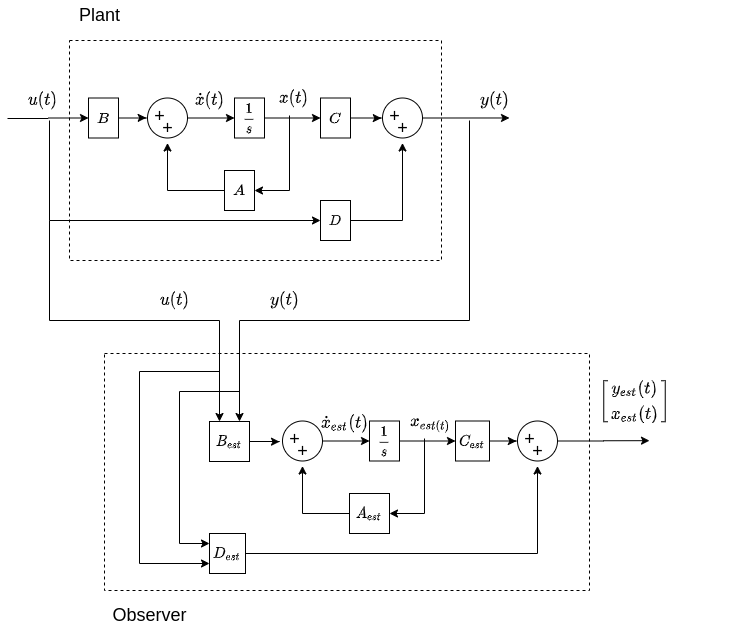
\includegraphics[width=0.7\textwidth]{Chp2/plant_observer.png}
	\caption{ Scheme of a state-space model plant and its observer or state estimator. \label{plant_obser}}
\end{figure}

Kalman filters have the structure of an ordinary state estimator but they take into account the process and measurement noise($\omega_d\,,\omega_n$) from the inputs signals. In Kalman filters the optimal choice of $K_{obs}$, which minimizes  the covariance $E{[x-x_{est}]^T~[x-x_{est}]}$, is given by(~\cite[Chapter~9]{Skogestad},~\cite[Chapter~8]{Hippe2009}):  

\begin{equation}
K_{obs}=Y~C^T~V^{-1}
\label{K_obs}
\end{equation}
 where $Y=Y{ T}~ \geq 0$ is the unique positive-semidefinite solution of the algebraic Ricatti equation:
 
 
\begin{equation}
YA^T~+~AY~-~YC^TV^{-1}CY~+W=0
\label{Ricatti2}
\end{equation}

where $W$ is a positive-definite Hermitian or real symmetric matrix and $V$ is a positive-definite Hermitian or real symmetric matrix, solving equation ~\ref{Ricatti2} for Y and substituting on ~\ref{K_obs}, gives the optimal $K_{obs}$ for reconstructing the states of the original system. The combination of an optimal state estimator or Kalman filter  and an optimal state feedback or LQR controller is commonly called LQG, this type of compensator-estimator configuration will be used ahead for implementation of plasma position controllers. 

\subsection{Experimental identification of state-space models}
\label{data_drivenSec}
When experimental work is carried out most of the times the available signals are not continuous. In addition it may happen that a theoretical model  linking experimental signals as inputs and outputs of it does not exist or has not been modeled yet. This section will address the representation in discrete time of state-space models as well as a method for retrieving a model based on experimental data  along with some useful concepts.
\smallskip

For some physical systems it is natural to work with the continuous-time representation of the systems since most of the basic relationships are expressed in terms of differential equations. The relation between the Laplace transform of the input and output of the system  is called \textit{transfer function} and is represented as $Y(s)=G_C(s)U(s)$, where introducing $p$ as the differential operator the time-domain transfer function yields as:  $y(t)=G_C(p)u(t)$. Taking into account the disturbances that influence  the system the transfer function can be re-written as: $y(t)=G_C(p)u(t)+H(q)w(p)$ ~\cite[Chapter~2]{Ljung1987}. Thus, the discrete transfer function will be $G_C(p) \rightarrow ~G_T(q)$  where $q$ is the discrete time shift operator, for the state-space models variables $G_T$ and $H$ are matrices. The concept of transfer function will be frequently used in this section.
\smallskip


\subsubsection{State-Space discrete models}
When implementing numerical methods and models in digital computers it is necessary to transfer the continuous variables and models to their discrete equivalents. If an input $u(t)$ is generated by a digital computer followed by a digital to analog converter (DAC), then $u(t)$ will be piecewise constant, this situation often arises in computer control of control systems~\cite[Chapter~4]{Chen1999}. Let:
\begin{equation}
u(t)=u(kT)=:u[k] \qquad for\: kT\leq~t~<(k+1)T
\end{equation}
for $k=0,1,2,..$, where $T$ is the sampling time. This input $u[k]$ changes values only at discrete time instants. If an input changes its value only at discrete time instants $kT$ and the response is only computed at $t=kT$ then discrete state-space model (considering absence of disturbances ) can be represented as:


 \begin{align}
x[k+1]=A_d[k]~+~B_du[k]\\
y[k]=C_dx[k]~+~D_du[k]
\label{SS_dscrt}
\end{align}
with
\begin{equation}
A_d=e^{AT}\qquad B_d=\left(\int_{0}^{T} e^{A\tau}d\tau\right)B \qquad C_d=C \qquad D_d=D \, .
\end{equation}



\subsubsection{Discrete state-space model identification}
\label{Disc_SS_ident}
For system identification purposes it is often desirable to use parametric models, i.e., a set of models is described by a number of real-valued parameters collected in a parameter  vector $\theta\in \mathbb{R}^d$ to be determined. A particular model is then represented by a value of the d-dimensional unknown parameters vector $\theta$ ~\cite[Chapter~2]{McKelvey1995}. Let's write the state-space model structure considering the discrete disturbances $w[k]$ in the form:

\begin{equation}
\mathcal{M}:\quad
\begin{aligned}
\hat{x}[k+1]&= A(\theta)\hat{x}[k] + B(\theta)u[k] + E(\theta)w[k] \\
y[k]&=C(\theta)\hat{x}[k]+w[k]
\end{aligned}
\label{M:}
\end{equation}

\noindent where  the vectors $\hat{x}$ and $\hat{y}$ are called predictors and they are the conditional expectations of $x(t)$ and $y(t)$ given information up to $k-1$ and the matrices A,B,C and E are constructed from the parameter vector $\theta$ according to the model structure $\mathcal{M}$. Let:

\begin{equation}
d_{\mathcal{M}}=dim ~\theta
\end{equation}
 denote the dimension of the parameter vector $\theta$ and let $\mathcal{M}(\theta)$ denote the model from equation ~\ref{M:}. The way of representing the disturbances in ~\ref{M:} is called the innovations form. The model will thus have the transfer functions:
 \begin{equation}
 G(q,\theta)=C(\theta)[qI-A(\theta)]^{-1}B(\theta)
 \end{equation}
 and
 \begin{equation}
 H(q,\theta)=I+C(\theta)[qI-A(\theta)]^{-1}K(\theta) \quad .
 \end{equation}

From equation ~\ref{M:}, the state predictor $\hat{x}[k+1]$ is given by:

\begin{equation}
\label{predictor}
\begin{aligned}
\hat{x}[k+1]&=[A(\theta)-K(\theta)C(\theta)]\hat{x}[k]~+~B(\theta)u[k]~+~-K(\theta)y[k] \\
\hat{y}[k|\theta]&=C(\theta)\hat{x}[k]
\end{aligned}
\end{equation}
 where  $\hat{y}[k|\theta]$ denotes the conditional expectation of $y[k]$ given the parameter vector $\theta$ ~\cite[Chapter~3]{Ljung1987}, this is a one-step ahead prediction and is denote as $\hat{y}[k|\theta]$ to emphasize its dependence on the parameter vector $\theta$.\smallskip
 
The system identification technique  applied is based on the prediction error minimization (PEM) ~\cite[Chapter~7]{Ljung1987}, ~\cite[Chapter~3]{Ljung1987}. The standard setting can be described as: given the experimental data consisting of an input vector {u[k]} and an output vector {y[k] } by:

\begin{equation}
Z^N~= \{y[k],u[k]|k=1,...,N\}, 
\end{equation}
 
\noindent and a model structure $\mathcal{M}$ defining  a mapping from the parameter space $D_{\mathcal{M}}$ to the outputs predictor $\hat{y}(t|\theta)$, the objective is to find the value $\hat{\theta}$ which minimizes a criterion $V_N(\theta)$. This criterion is defined as:
 \begin{equation}
 V_N(\theta)=\frac{1}{N} \sum_{t=1}^{N}|\varepsilon[k,\theta]|^2,
 \label{V_N}
 \end{equation}
 
 where $|\cdot|$ is the Euclidian $l_2-norm$. The prediction error is the vector
 \begin{equation}
 \varepsilon(t,\theta)~=y[k]-\hat{y}[k|\theta]
 \end{equation}
 with the predictor $\hat{y}(t|\theta)$ given by the equation ~\ref{predictor}. The minimizing parameter vector is defined by:
 \begin{equation}
 \hat{\theta}_N=\argmin_{\theta \in D_\mathcal{M}}~V_N(\theta)
 \end{equation}
 
\noindent where "arg min" is the operator returning the argument which minimizes the function. The minimization of $V_N(\theta)$ given in equation ~\ref{V_N}  as well as the properties of the resulting estimation of the parameters vector $\hat{\theta}_N$ under varying assumptions on the model structure $\mathcal{M}$ and the experimental data set $Z^N$, has been formulated in the related literature and computationally implemented, such is the case of the \textit{System Identification Toolbox} from \textsc{Matlab}. This toolbox relies on the function called "pem" for computing the error minimization which returns an estimated state-space model given a data vector of input and output signals\cite[Chapter~4]{Toolbox}, the model is adjusted by optimizing the prediction error fit, it is possible to select the order of the model or use the "best" order given by the toolbox. Due to its adaptability and flexibility, this toolbox was used for retrieving data-driven models in several stages of the implementation of real-time control algorithms in ISTTOK.

\chapter{JT-60SA control design}

The current chapter is completely  focused on the magnetic control for  the JT-60SA tokamak  plasma position and shape. Different proposed  controllers  are applied  on a particular flat-top scenario in order to reject a set of given disturbances. Through the models retrieved by the CREATE tools it was possible to design a controller of the plasma parameters with the so-called eXtreme Shape Controller (XSC) approach, this controller is compared with the implemented QST control and reconstructions tools.   

\section{Machine description}

JT-60SA is a superconductive tokamak located at one of the facilities from the National Institutes for Quantum and Radiological Science and Technology (QST)  at  Naka, Japan whose principal purpose is  the contribution to early realization of fusion energy by supporting the exploitation and resolving key physics for the ITER reactor.  JT-60SA construction has been successfully completed by the end of March 2020 and its first plasma is expected for late 2020. Figure ~\ref{JT60schm} shows the overall general configuration and the most remarkable elements of the machine. The JT-60SA  vacuum chamber will have a major radius of 2.96~ m and a Minor radius of 1.18~ m with an overall plasma volume of 132~ $m^3$ ~\cite{Spears2014}. JT-60SA will become the largest tokamak ever built so far. Appendix ~\ref{JT60_append} contains a set of photos depicting the assembling of some of the JT-60SA components and its overall look during 2018 and 2019. 
\smallskip

\begin{figure}[h]
	\centering
	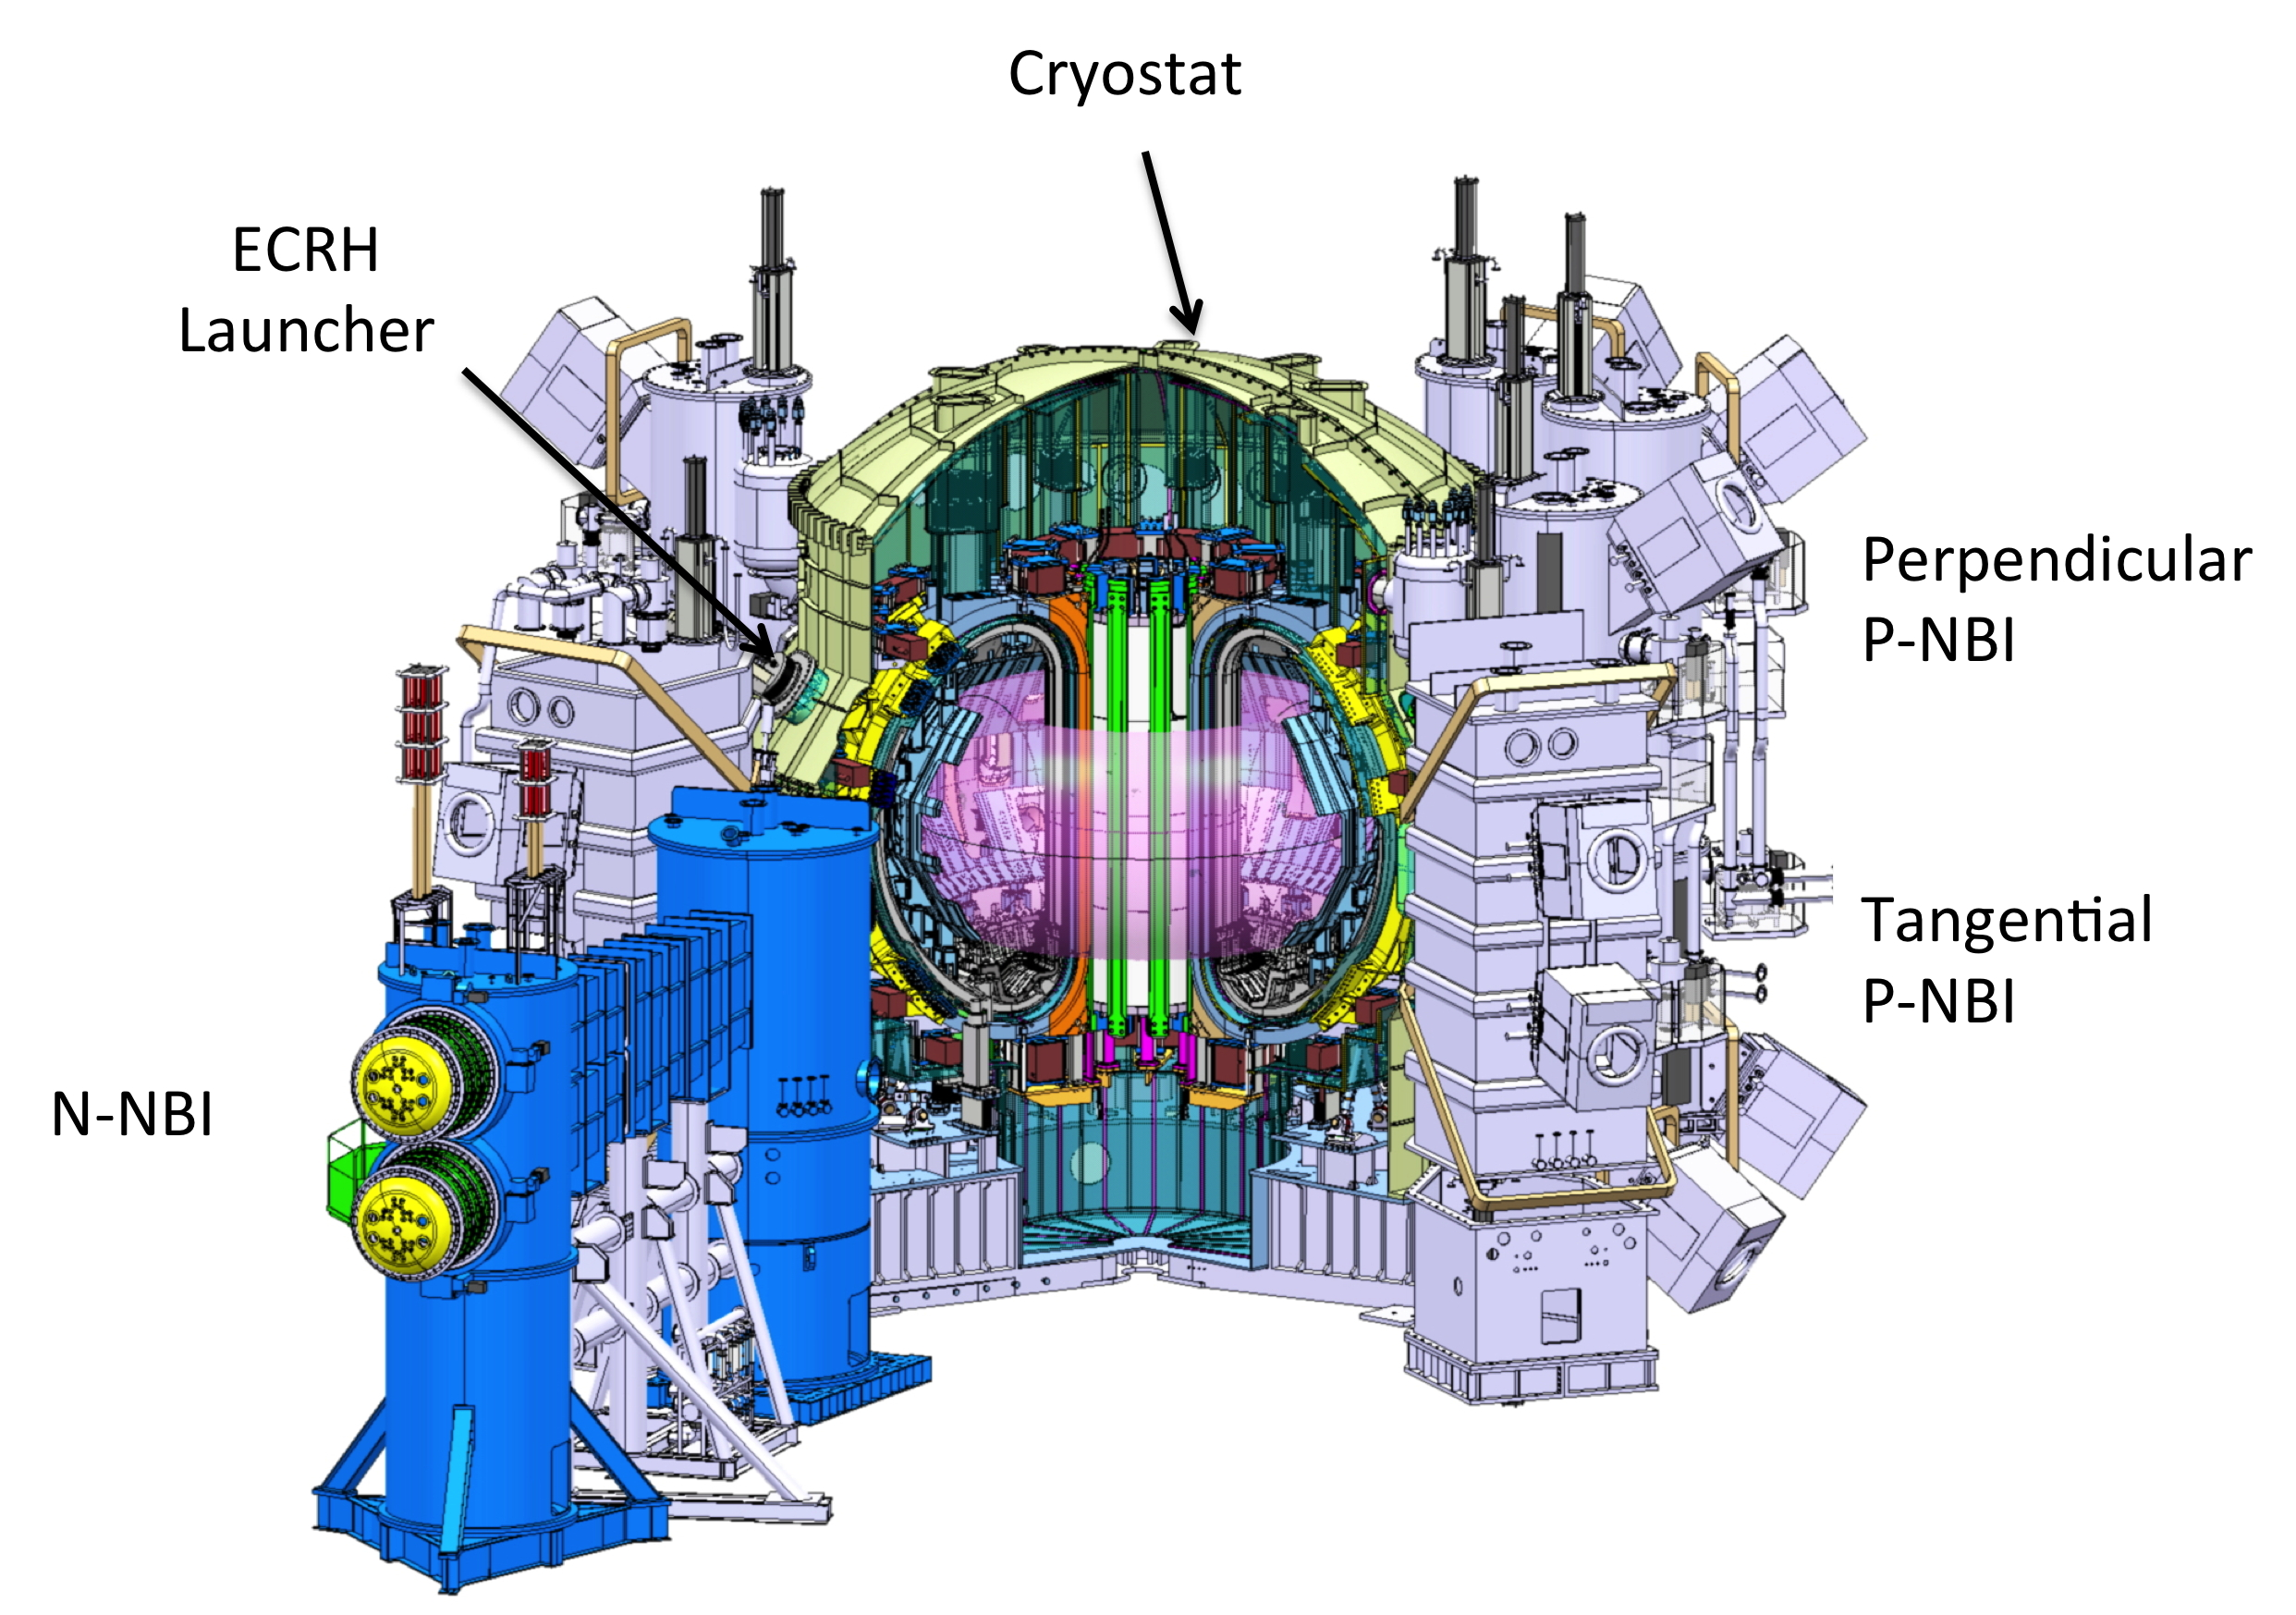
\includegraphics[width=0.75\textwidth]{Chp3/JT60SA.png}
	
	\caption{\label{JT60schm}JT-60SA tokamak configuration and its main elements ~\cite{JT60SA:ResearchPlan}.}
\end{figure}

The Poloidal Field (PF) coils shown in JT-60SA cross-section from figure ~\ref{JT60coils} consist of two sets of superconductive coils: the Equilibrium Field Coils (EF1–6) and the Central Solenoid (consisting of four independent coils, named CS1–4) which are ex-vessel coils. Furthermore, two in-vessel cooper Fast Plasma Position  Coils (FPPC1–2) will also be installed ~\cite{NCruz}. The total of 12 PF coils have independent power sources for the control of the plasma current, position and shape.   
\smallskip

\begin{figure}
	\centering
	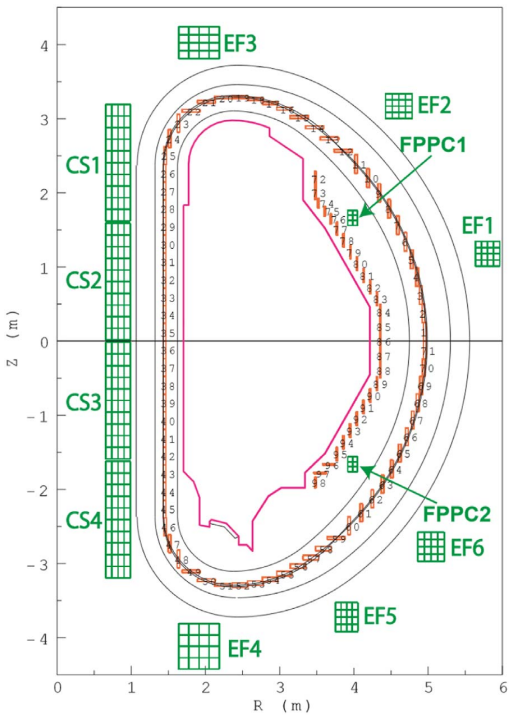
\includegraphics[width=0.55\textwidth]{Chp3/JT60Coils.png}

	\caption{	\label{JT60coils}JT-60SA poloidal cross-section and layout of the Poloidal Field coils system ~\cite{NCruz}.}
\end{figure}

JT-60SA shall be capable of investigating different design scenarios. As refereed  in 
~\cite{JT60SA:PID} it exists a set of 6 reference scenarios, additional ones, including some with a shorter repetition rate will be defined in future. For the control study in this section all simulations will be built based on the Scenario~2 characteristics. In particular, Scenario~2 refers to a~5.5 MA inductive lower single null discharge. The Scenario~2 its divided in 5 time snapshots with different equilibrium each one starting at  t=-40~s until t=~177.96~s. The different Last Closed Flux Surfaces (LCFS) for each time window are shown in figure~\ref{Scen2}, the time sequence starts at the X-point formation (XPF)	followed by the Start of Heating (SOH), the Start of Flattop (SOF), End of Flattop (EOF), End Of Cooling (EOC) and finishing with the End of Currents in the PF coils (EOC). In this section, reconstruction methods and control algorithms will be based on the \emph{Start of Flattop}~(SOF) equilibrium shown in figure~\ref{SOF}. The nominal values for the plasma current, the poloidal beta and the internal inductance for Scenario~2 at SOF are~$I_{p_{eq}}~=~5.5$~MA,~ $\beta_{p_{eq}}=0.53$, and~$l_{i_{eq}}=0.85$.\smallskip

\begin{figure}[h]
	\centering
	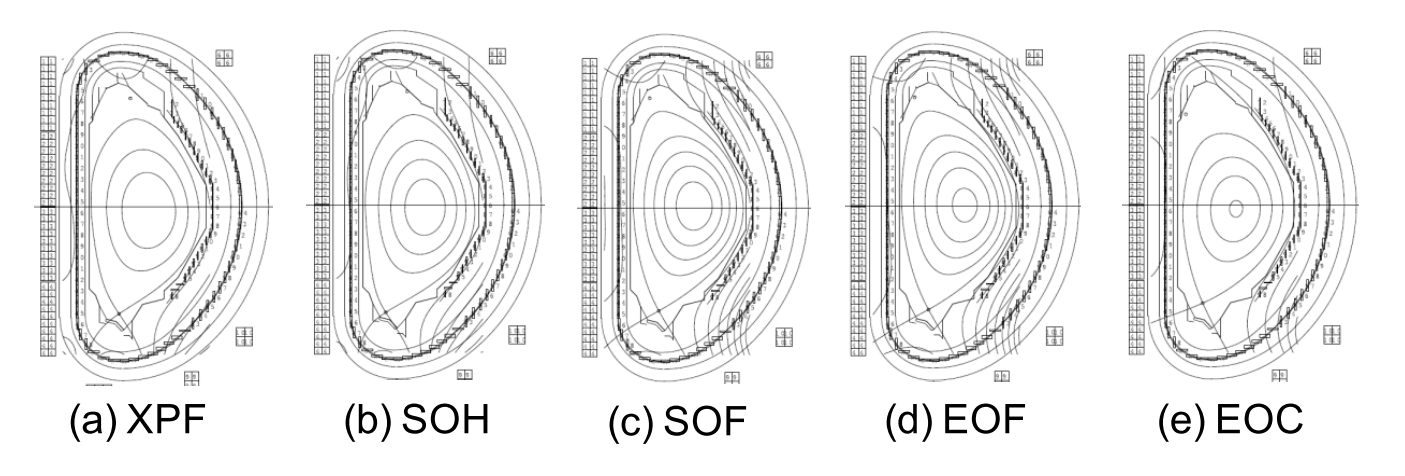
\includegraphics[width=0.99\textwidth]{Chp3/scenario2SnapShots.png}
	
	\caption{LCFS Equilibria corresponding to the different Scenario~2 snapshots:  X-point formation (XPF), Start of Heating(SOH), the Start of Flattop (SOF), End of Flattop (EOF), End Of Cooling(EOC) and  End of Currents in the PF coils (EOC) ~\cite{JT60SA:PID}. \label{Scen2}}
\end{figure}


\begin{figure}[h]
	\centering
	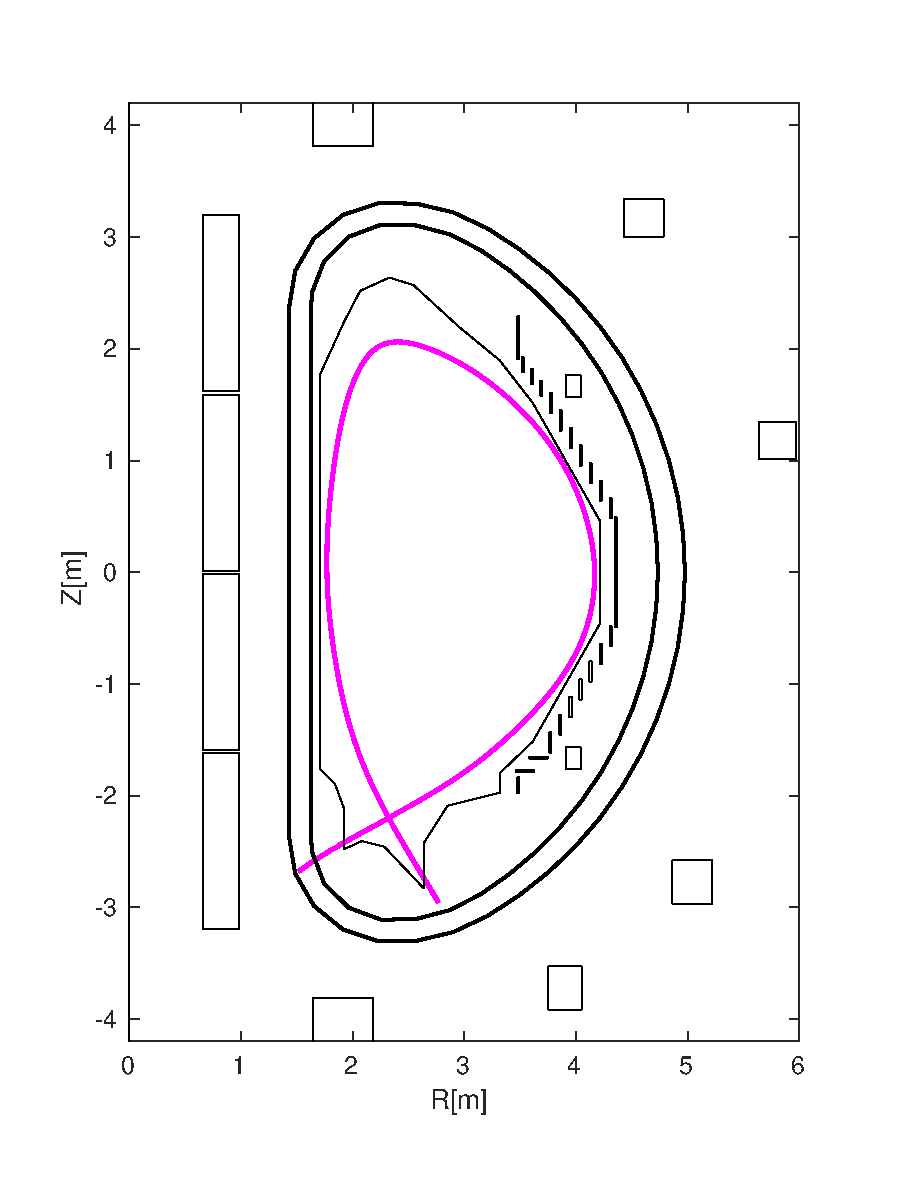
\includegraphics[width=0.5\textwidth]{Chp3/scenario2_SOF.eps}
	
	\caption{Poloidal cross-section of the JT-60SA plasma at the Start of the Flat Top~(SOF) for reference Scenario~2. At SOF, the nominal plasma current is ~5.5~MA, while the nominal values for poloidal beta~$\beta_p$ and internal inductance~$l_i$ are~0.53 and~0.85, respectively.	\label{SOF}}
\end{figure}



This chapter will address two different approaches for the LCFS reconstruction along  with different plasma current, shape and position controllers for JT-60SA in order to achieve and maintain the desired operational scenario given the plasma equilibrium in the SOF while the performance of the controllers is compared.



\section{CREATE magnetic modeling tools}

CREATE-NL  is a finite elements method (FEM\footnote{It is well known that many physical and engineering systems are expressed in terms of partial differential equations which cannot be solved via analytical methods. One of the most recurrent techniques is numerical discretization to approximate the solution of the partial differential equations, the FEM is commonly used to solve these approximations in two or three space variables, in this particular case for a numerical solution of the well-known Grad-Shafranov equation. }) solver implemented on \textsc{Matlab}. It deals with the free boundary dynamic plasma equilibrium problem i.e. the MHD (Magneto-Hydro-Dynamics) time evolution of 2D axisymmetric plasmas in tokamaks, including eddy currents in the passive structures, and feedback control laws for current, position and shape control ~\cite{Albanese:CREATENLnew}. CREATE-NL is an upgraded version of the CREATE-L code written in FORTRAN and validated in different tokamaks. Both CREATE-L and CREATE-NL produce linerized models of the plasma in the neighborhood of a certain equilibrium condition. CREATE-NL has more capabilities than CREATE-L due to the possibility of using different plasma profiles shapes,  introducing different outputs in a user friendly way and  running inverse equilibrium calculation~\cite{DeTommasi2007}. 
\smallskip

Using the CREATE codes~\cite{Albanese:CREATEL,Albanese:CREATENLnew} it is possible to retrieve a linearized state-space model for a reference configuration that describes the plasma magnetic behavior around that equilibrium\footnote{Reference  ~\cite[Sec.~3]{NCruz} can be consulted for more details about the use of the CREATE equilibrium codes to retrieve plasma linearized models.}. It should be noted that CREATE-NL equilibrium solver has been validated on several tokamaks such as JET and EAST. A JT-60SA CREATE-NL electromagnetic linear model around the equilibrium from the Scenario~2-~SOF  for the plasma-circuit response has been used for  designing  the controller presented in next section. 
\smallskip






\section{Controller design}

The JET (Joint European Torus) tokamak was the first machine where around 2005 a new model based plasma current and shape controller was set up and tested  with the existing active circuits and control hardware. The novelty controller was the eXtreme Shape Controller (XSC) and its aim was to improve  the performance of the, back then, present controller to allow the control of extremely shaped plasmas with higher values of elongation and triangularity ~\cite{Albanese2005}. More recently this control approach was utilized at TCV ~\cite{anand2017novel}. At JET, the XSC  enabled the control of high triangularity shapes with both strike points in the divertor corner, which has a large impact in the H-mode confinement in the case of the ITER-like wall at JET~\cite{de2016recent}, ~\cite{Albanese2005}.   The XSC approach has been recently validated at the EAST tokamak during the 2019-2020 campaigns where the proposed XSC controller proved to be effective in rejecting the disturbances induced  ~\cite{EAST2020}.
 \smallskip
 
 Usually the controlled shape geometrical descriptors are the distances between the plasma boundary and the vessel at some specific points. These plasma-wall distances are called gaps ~\cite{Ambrosino:TCST2008}. The gaps are segments that can be used to describe the shape of the plasma boundary. Being~$g_i$ the abscissa along the~$i$-th control segment, we assume that~$g_i=0$ at the first wall. \emph{Gap-based} plasma shape control is achieved by controlling to zero the difference $g_{i_{ref}}-g_i$ on a sufficiently large number of gaps, being~$g_{i_ref}$ the value of the abscissa on the~$i$-th control segment for the reference shape. Figure ~\ref{figure:85_gaps} shows a poloidal cross-section of JT-60SA together with a set of 85 gaps used for the assessment of the plasma shape control.
 \smallskip
 
 \begin{figure}[h]
 	\begin{center}
 		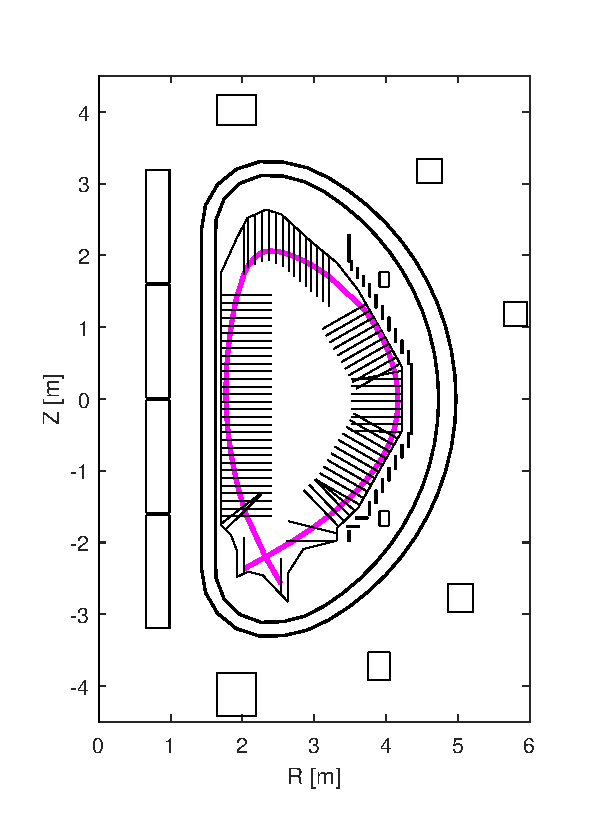
\includegraphics[width=0.45\textwidth]{Chp3/85_gaps_2.eps}
 	\end{center}\caption{Poloidal cross-section of the JT-60SA plasma at the Start of the Flat Top~(SOF) for reference Scenario~2. At SOF, the nominal plasma current is~5.5~MA, while the nominal values for poloidal beta~$\beta_p$ and internal inductance~$l_i$ are~0.53 and~0.85, respectively. In this figure the~85 gaps used to assess the plasma shape controller performance are shown.}\label{figure:85_gaps}
 \end{figure}
 
  The XSC algorithm can be used either to implement a gap-based control strategy, or an isoflux one, as it has been proposed in ~\cite{NCruz}. The isoflux strategy consists in controlling the X-point position along with a set of flux differences between the flux at some selected control points along the desired plasma boundary and the X-point flux. Thus the XSC block inputs are the error between the X-point flux and the fluxes in the control points, and the X-point position error.
\smallskip


The peculiarity of the XSC approach is that it, this  is basically tackled by using a singular value decomposition (SVD) to identify the principal directions of the algebraic mapping between coil currents and geometrical descriptors ~\cite{Albanese2005}. The XSC control relies on the PFC decoupling controller (more details can be found in~\cite[Section~4.4]{NCruz}), since it is assumed that each~PF coil can be treated as an independent single-input-single-output (SISO) channel whose dynamic response is modeled in the Laplace domain by
\[
I_{PF_i}(s) = \frac{I_{PF_{ref\,,i}}(s)}{1+s\tau_{PF}}\,,
\]
where~$I_{PF_i}$ and~$I_{PF_{ref_i}}$ are the Laplace transform of the measured and reference current in the~$i$-th PFC, respectively, and where it is assumed that all the PFC exhibit the same bandwidth (i.e.,~they have the same time constant~$\tau_{PF}$).
\smallskip

Denoting by~$\delta Y(s)$ the Laplace transform of the variations of the~$n_G$ shape descriptors  to be controlled, it is possible to exploit the CREATE electromagnetic linear model~\cite{NCruz} that links the variation of the PFC reference currents~$\delta I_{PF_{ref}}$ to ~$\delta Y(s)$, i.e.
\[
\delta Y(s) = C\frac{\delta I_{PF_{ref}}(s)}{1+s\tau_{PF}}\,,
\]
which, at steady-state, implies~ $\delta Y(s) = C \delta I_{PF_{ref}}(s)$.

If the number of controlled plasma shape descriptors~$n_G$ is such that~$n_G~>~n_{PF}$, the XSC computes the additional current references as
\begin{equation}\label{equation:XSC_new}
\delta I_{PF_{ref}}(s)=C^\dag\delta Y(s)\,.
\end{equation}
where the matrix~$C^\dag$ denotes the pseudo-inverse of~$C$\footnote{$C$ ~ is the output matrix from the state-space linearized CREATE model for JT-60SA.} that can be computed via the singular value decomposition (SVD). As a result, the XSC algorithm minimizes the following steady-state performance index
\begin{equation}\label{equation:XSCcost}
J_{XSC} = \lim_{t\to +
	\infty}(\delta Y_{ref}-\delta Y(t))^T(\delta Y_{ref}-\delta Y(t))\,,
\end{equation}
where~$\delta Y_{ref}$ are constant references for the geometrical descriptors. When the SVD of the~$C$ matrix is used to minimize~\eqref{equation:XSCcost}, it may happen that some singular values (depending on the plasma configuration) are one order of magnitude smaller than the others. This fact implies that minimizing the performance index~\eqref{equation:XSCcost} retaining all the singular values results in a large control effort at the steady-state, that is a large request on some PFC currents which have only a minor effect on the plasma shape. In order to minimize also the control effort, the additional references~\eqref{equation:XSC_new} are generated by using only the~$\bar{n}<n_{PF}$ linear combinations of PF currents which are related to the largest singular values of the~$C$ matrix. This is achieved by using only the~$\bar{n}$ singular values when computing the pseudo-inverse~$C^\dag$.
\smallskip

Moreover, the PFC current variations given by~\eqref{equation:XSC_new} are summed to the scenario currents and sent to the PFC decoupling controller as references to be tracked. It is worth to remark here that the dynamnic behavior of the XSC is improved by adding a set of proportional-integral-derivative (PID) controllers on each PF coil channel (see~\cite{Ariola:XSC} for a complete description of the XSC control scheme).
\smallskip

For the development of this work both approaches of the XSC strategy were studied and simulated for a different number of control points: isoflux and gap-based controllers. In addition, a second controller developed by the QST team was implemented in the simulations, the features of this controller will be detailed in the next section.



\section{QST reconstruction and control implementation}
Along with the CREATE modeling tools presented on last section, which allow to compute the LCFS and to apply model-based design to compute the XSC, a reconstruction code and controller provided by the QST team were implemented, tested and compared. This section will briefly describe these two methods and its limitations.  

\subsection{Cauchy Condition Surface (CCS) reconstruction  method }
The QST Cauchy Condition Surface (CCS) method for the reconstruction of the magnetic last closed flux surface (LCFS) calculates controlled variables for plasma position and shape control such as the poloidal magnetic flux at control points on an isoflux scheme  ~\cite{CCS}. The CCS method allows a selection up to 19 geometrical points for describing the LCFS and its input parameters are the currents in the PF coils, the measurements in the magnetic field and flux sensors and the plasma current. The output signals from the CCS reconstruction method are the magnetic fluxes at the X-point and at the selected geometrical points. 

\begin{figure}
	\centering
	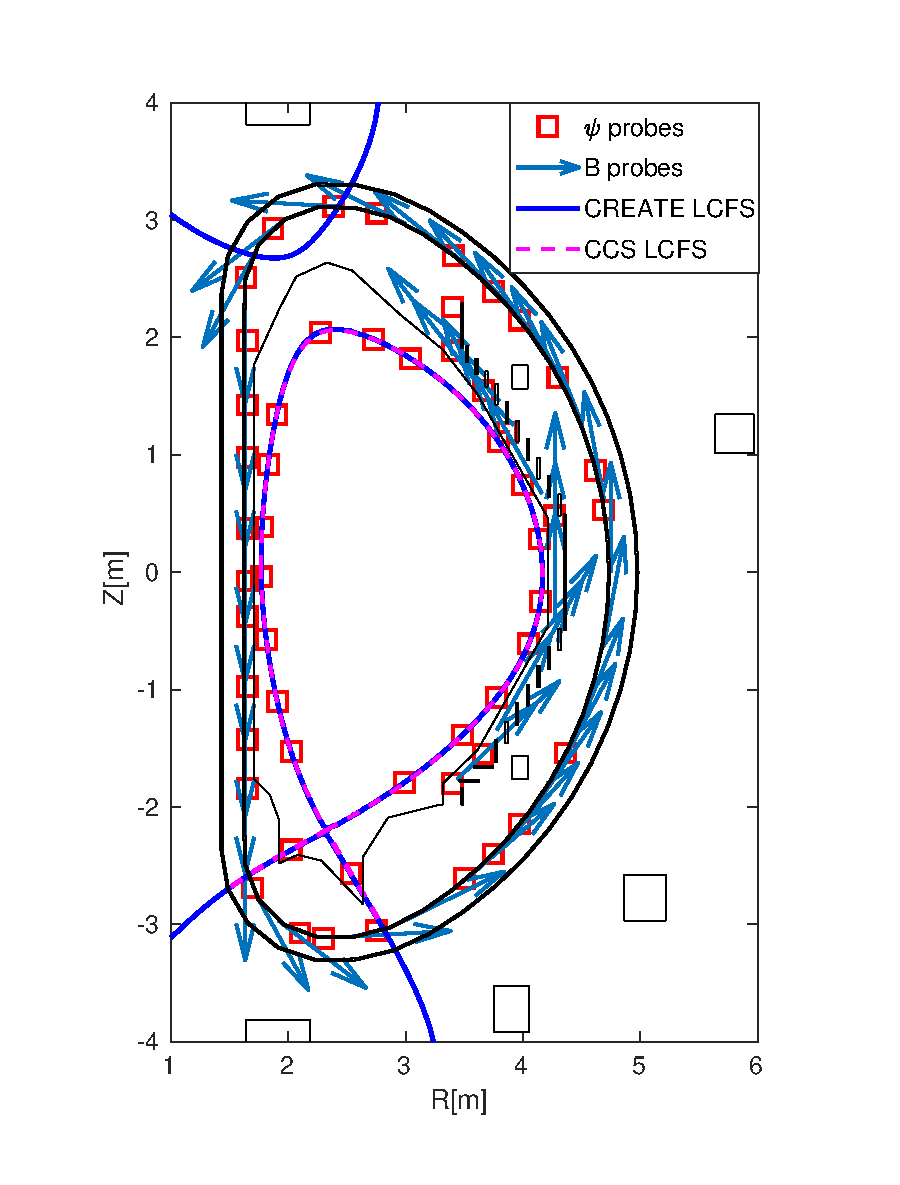
\includegraphics[width=0.6\textwidth]{Chp3/sensors_plots_newDirection.eps}
	\caption{SOF equilibrium reconstructed from CREATE-NL and the CCS code along with the  magnetic field and flux sensors locations.	\label{JT60sensors} }
\end{figure}


\subsection{QST magnetic controller }


The QST magnetic controller  uses the PF coils signals to control the plasma current $I_p$, position and shape, and the FPPC coils signals for plasma position control. The PF coil currents $I_{PF-ref}$ are calculated using an isoflux control approach using proportional-integral(PI) feedback controllers   ~\cite{FBC}. The controller calculates $I_{PF-ref}$ reducing $\delta\Psi_s$ and $\delta\Psi_x$ according to:



\begin{equation}
I_{PF\_ref}(t+\Delta t) = I_{PF}(t_0)+M^\dagger_{PF}\left[G_{SP}\delta\Psi_s(t)+G_{SI}\int_{t_0}^{t}\delta\Psi_s(t)dt+G_{XP}\delta\Psi_X(t)+G_{XI}\int_{t0}^{t}\delta\Psi_x(t)dt\right]~,
\end{equation}

where $\delta\Psi_s$ is the residual between the  LCFS flux and the control point fluxes,   $\delta\Psi_x$ is the difference between the $I_p$ value and its reference, $t_0$ is the initial time, $\Delta t$ is the coil control cycle, $M^\dagger_{PF}$ is the (m $\times$ (n + 1)) control matrix which is the pseudo-inverse of the Green function $M$ calculated using the SVD method; where m is the number of PF coils, n is the number of control points including the evaluated X-point. $G_{SP}$ and $G_{SI}$ are the respective control gains for the PI plasma position and shape feedback controllers, $ G_{XP}$ and $G_{XI}$ are the PI control gains for the $I_p$ feedback control. $G_{SP}$ and $G_{XP}$ are dimensionless and, $G_{SI}$ and  $G_{XI}$ are in $s^{-1}$. \smallskip



The coils voltage command values ($V_{coil-com}$) are calculated considering the mutual interactions between the PF coils an the plasma, the actual values of the PF coil currents, $I_p$ and the mutual inductances. On a real plasma experiment, the  mutual inductances between the plasma and the PF coils are unknown due to the difficulty of measuring them directly. Therefore, they are provided by the CCS method. The controller calculates command values of PF coils voltages according to the following equation:



\begin{equation}
V_{com}=G_{vt}\left[M_{coil}\frac{(I_{coil\_ref}-I_{coil\_meas})}{dt}+ \frac{M_{plasma\_now} \cdot I_{p\_now} - M_{plasma\_ bfr} \cdot I_{p\_bfr}}{dt}\right]~,
\end{equation}

where $M_{coil} $ represents the mutual inductances between the coils, $I_{coil\_meas}  $ are the measured coil currents,  $M_{plasma\_now}$ and $ M_{plasma\_ bfr}$ are the mutual inductances between the plasma and the coils at the current and previous time step,$  I_{p\_now} $  and  $ I_{p\_bfr} $ are the measured plasma current at the current and previous time step  and $ G_{vt} $ is the voltage transformer gain.
\smallskip

On the other hand,the in-vessel FPPC coils currents $ (I_{FPPC\_ref})  $ are calculated with an isoflux control approach which uses proportional-differential (PD) feedback control. In order to reduce  the residual between the LCFS flux and two specified control points ( $ \Psi_{SF} $)  the controller calculates  $ (I_{FPPC\_ref})  $ using:

\begin{equation}
I_{FPPC\_ref}(t+\Delta t)=I_{FPPC}(t_0)+ M^\dagger_{FPPC}\left[G_{FP}\delta \Psi_{SF}(t) + G_{FD}\frac{d}{dt}\delta\Psi_{SF}(t) \right] ~,
\end{equation}

where $ M^\dagger_{FPPC}$ is the $ 2 \times 2$ control matrix which is the pseudo-inverse of the Green function $M_{FPPC}$, $ G_{FP} $ and $ G_{FD} $
are the respective PD feedback gains for the plasma position control. $ G_{FP} $ is dimensionless and $ G_{FD} $ is in $s$.



\section{Simulation results}	

 The simulations for  the JT-60SA CREATE-NL model,the XSC, the CCS reconstruction method and the QST controller  were programmed on top of  \textsc{Matlab} and \textsc{Simulink} blocks. This  section will address in detail the outcome of the control simulations using a linearized equilibrium given by CREATE-NL for JT-60SA, Scenario~2 at the SOF time frame. The first results to be presented correspond to a  gap-based controller  using the XSC with different tests cases.
 \smallskip
 
 
 The second part of the results corresponds to isoflux controllers using the XSC  with a LCFS reconstruction given by the fluxes retrieved by the CREATE model and also given by the CCS method, as well as the QST controller with the LCFS reconstructed by the CCS method and by CREATE. The figures ~\ref{JT60controlscheme} and ~\ref{JT60FBCcheme} show an overall control block scheme for the simulations.   Figure ~\ref{JT60controlscheme} corresponds to a configuration using the XSC where the LCFS can be obtained through the CCS method or from the CREATE model. It is worth to point out the existence of the block localized on the bottom part of the scheme called "Vertical Stability Control" along with the XSC. The task of this block is to vertically stabilize the plasma by exploiting the in-vessel coils, which are able to guarantee a faster response due to the fact that the magnetic field generated does not have to penetrate the vessel structures  ~\cite{NCruz}. This controller calculates the voltages at the FPPC coils with the equation:
 
 \begin{equation}
 V_{FPPC}(t)=k_1I_{FPPC}(t)+ k_2\dot{z}_p(t)
 \label{FPPC_eqs}
 \end{equation}   
 
 By tuning the gains $k_1$ and $k_2$ from equation ~\ref{FPPC_eqs} is possible to obtain zero velocity in the vertical plasma direction while maintaining low imbalance current $  I_{FPPC} $ in the in-vessel coils~\cite[Sec.~4.1]{NCruz}.  In addition should also be notice the block "Ip Control" which is a Plasma current Controller, which tracks the desired value of the plasma current ~\cite{de2014shape}.

 
 
\begin{figure}
	\centering
	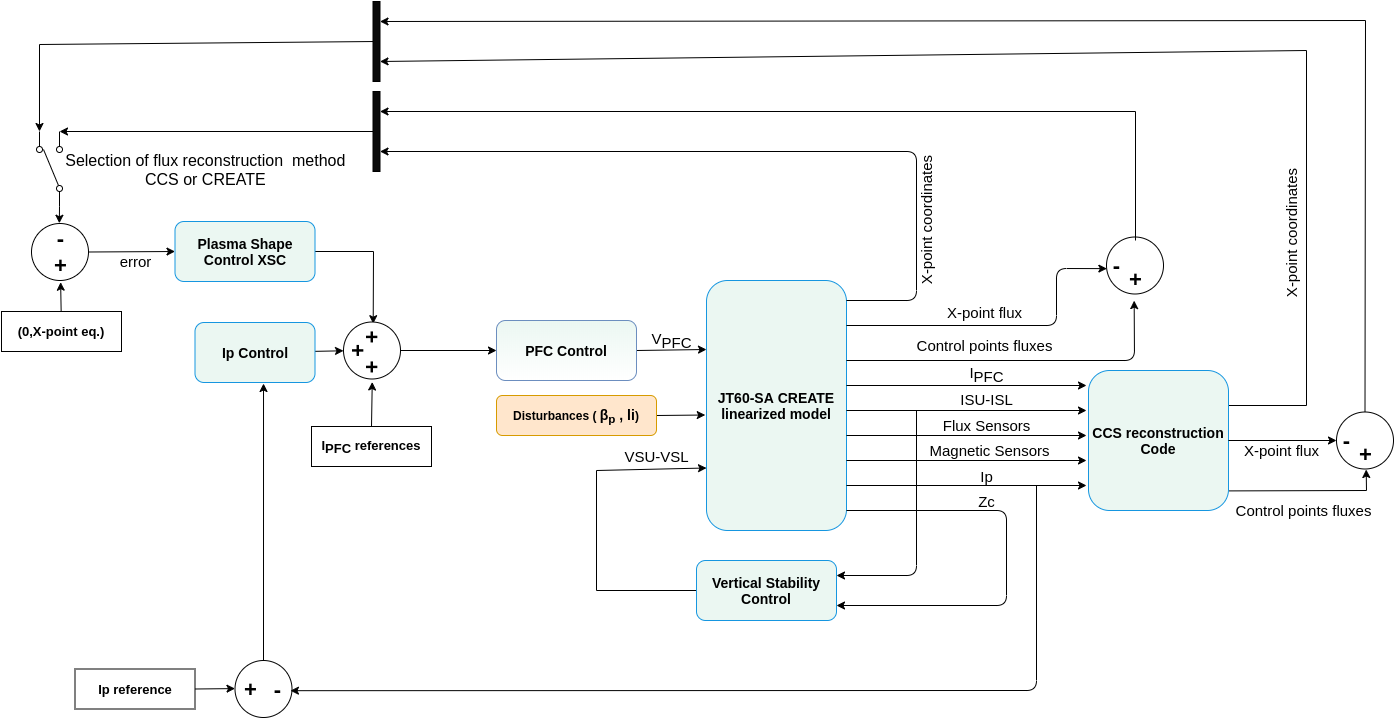
\includegraphics[width=1.05\textwidth]{Chp3/JT60Schemes1.png}
	\caption{	\label{JT60controlscheme}JT-60SA overall control scheme with the CREATE linearized model and the CCS LCFS reconstruction method  using the XSC for an isoflux control approach.}
\end{figure}

Figure ~\ref{JT60FBCcheme} depicts a configuration using the QST controller reciving as inputs the magnetic fluxes measured at the control points reconstructed either by the CCS method or by the CREATE linearized model.
\smallskip
 
\begin{figure}
	\centering
	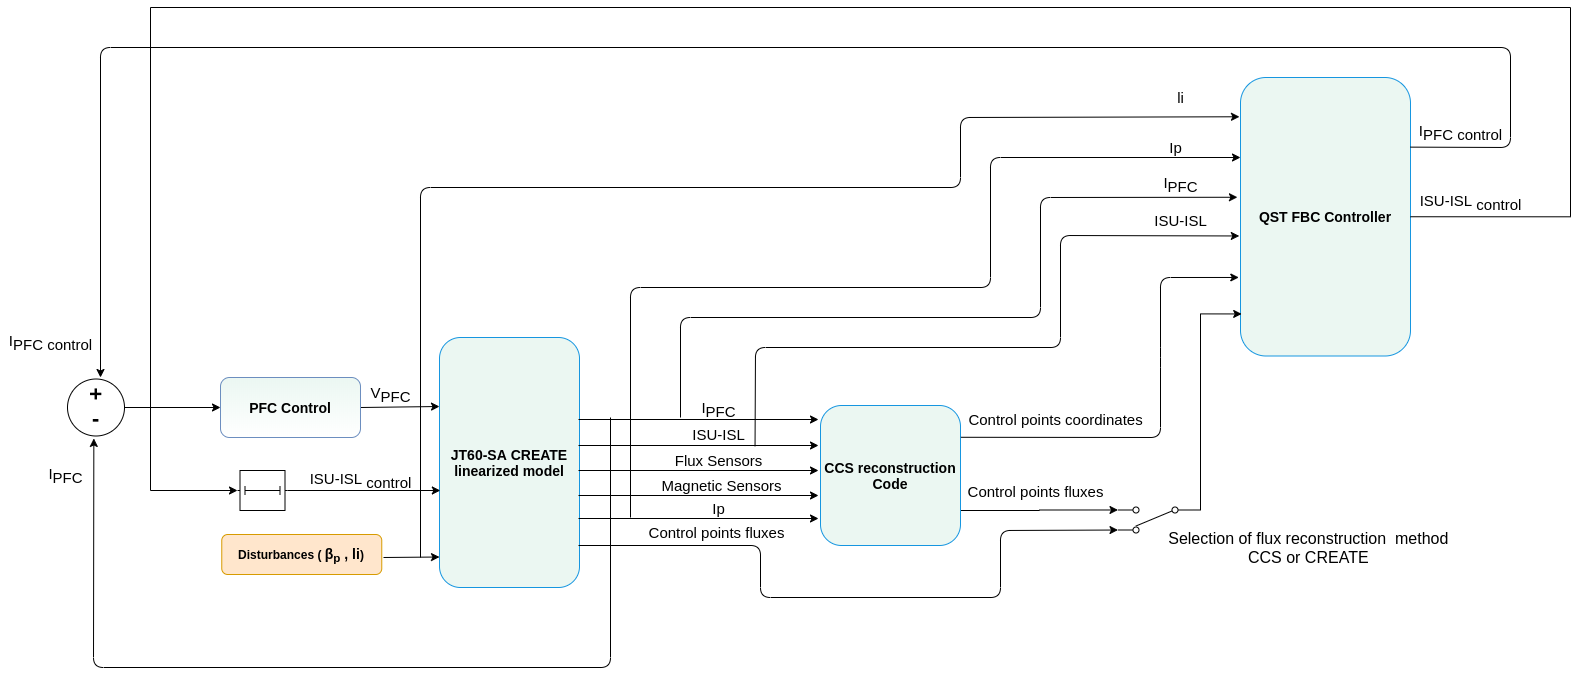
\includegraphics[width=1.05\textwidth]{Chp3/JT60SchemeFBCnew.png}
	\caption{	\label{JT60FBCcheme} Isoflux control JT-60SA overall scheme with  a block for the  CREATE JT-60SA linearized model, a block for reconstructing  the magnetic fluxes with the CCS method and the QST controller. }
\end{figure}



\subsection{Disturbances}


As far as plasma magnetic control is concerned, the JT-60SA linearized model disturbances have been modeled as variations of $\beta_p$ and $l_i$. This disturbances should be in principle rejected by the control systems and maintain in the most accurate possible way the plasma equilibrium.  The following set of disturbances have been considered: 

\begin{itemize}
	\item \textbf{Disturbance \#1} refers to the behavior of~$\beta_p$ and~$l_i$ soon after the current flattop is reached, as it was modeled in~\cite{urano2015development} (in this paper we assume that the flattop is reached at~$t\sim 20$~s). As an example, the correspondent time traces are shown in figure~\ref{Urano}\footnote{The time behavior of both~$\beta_p$ and~$l_i$ have been estimated starting from the spatial profiles for both plasma density and temperature envisaged for Scenario 2.}.
	
	


%	\item \textbf{Disturbance \#2} refers to the behaviour of ~$\beta_p$  due to the presence of an Edge-Localized Mode~(ELM). As described in~\cite[p.~34]{JT60SA:PID}, during the flattop an instantaneous drop in~$\beta_p$ of ~$0.05~\beta_{p_{eq}}$ is followed by and exponential recovery with a time constant of~0.05~s with a frequency 10~Hz. Note that for this disturbance~$l_i$ does not change.% remains as~$l_{i_{eq}}$, these behaviors are shown in Fig.~\ref{figure:ELM}.
	
	\item \textbf{Disturbance \#2} refers to the behaviour of~$\beta_p$ and~$l_i$ when a compound ELM\footnote{A compound ELM is commonly referred as multiple clearly distinguishable
	crash events causing large energy losses \cite{Meyer2017}.} appears during the flattop.  As described in~\cite[p.~34]{JT60SA:PID}, an instantaneous drop   in~$\beta_p$ of ~$0.05~\beta_{p_{eq}}$ is followed by and exponential recovery with a time constant of~0.05~s with a frequency 10~Hz, $l_i$ is described by an instantaneous drop of~$0.06~(l_{i_{eq}}-0.5)$ followed by and exponential recovery with a time constant of 0.05~s with a frequency 10~Hz. The time traces for~$\beta_p$ and~$l_i$ are described in figure~\ref{cmpELM}.
	


	
	\item \textbf{Disturbance \#3} describes an instantaneous drop in~$l_i$ of~$0.2~(l_{i_{eq}}-0.5)$ without recovery, simultaneous with a drop on~$\beta_p$ of~$0.2~\beta_{p_{eq}}$ followed by a recovery exponential time of~1~s~\cite[p.~34]{JT60SA:PID}, which are typical of a so called \emph{Minor disruption}. The correspondent time traces for both~$\beta_p$ and~$l_i$ are reported in figure~\ref{MnrDisrp}.
\end{itemize}


	\begin{figure}[h]
	\centering
	\includegraphics[width=0.5\textwidth]{Chp3/Dist_1_Urano.eps}
	\caption{Poloidal beta and internal inductance time traces for Disturbance~\#1 that models the expected disturbance soon after the plasma current flattop is reached (at~$t\sim 20 $~s), according to what has been considered in~\cite{urano2015development}.	\label{Urano} }
\end{figure}

	\begin{figure}[h]
	\centering
	\includegraphics[width=0.5\textwidth]{Chp3/Dist_2_cmp_ELM.eps}
	\caption{Poloidal beta and internal inductance time traces for Disturbance~\#2 that models the behavior of these variables due to the presence of a compound ELM as defined in~\cite{JT60SA:PID}.	\label{cmpELM} }
\end{figure}


\begin{figure}[h]
	\centering
	\includegraphics[width=0.5\textwidth]{Chp3/Dist_3_minor.eps}
	\caption{Poloidal beta and internal inductance time traces for Disturbance~\#3 that models the behavior of these variables due to the presence of a Minor disruption as defined in~\cite{JT60SA:PID}.	\label{MnrDisrp} }
\end{figure}



\subsection{Gap-based XSC}

JT-60SA represents a relevant benchmark to further validate the gap-based control approach, given the high beta regimes that are envisaged during its operation, which represent a challenge from the plasma magnetic control perspective. Different test cases are considered to assess the performance of the proposed shape controller, with the aim of defining an optimal set of gaps to be controlled. This sections evaluates the steady-state performance of the plasma shape controller under different choices for \emph{gaps} to be controlled. \smallskip

 All around the first wall an equally spaced distribution of~85 gaps was considered as shown in figure~\ref{figure:85_gaps}. It should be noticed that all different selections of controlled gaps considered in this paper include the two vertical gaps in the divertor zone, which allows to control the strike-points, and hence the position of the X-point. Other than the whole set of~85 gaps,  three additional choices are considered. The first one is reported in figure ~\ref{figure:20_gaps}, which consists of~20 gaps equally spaced along the first wall. Moreover, the selection of~8 and~6 gaps that correspond with the control segments considered by the isoflux controllers presented in~\cite{miyata2013study} and~\cite{Miyata:2014}, respectively, have been also considered (see  figures ~\ref{figure:8_gaps} and~\ref{figure:6_gaps}). These two latter options are the outcome of preliminary studies aimed at controlling the plasma shape with a set of almost decoupled loops, i.e.  SISO, while the XSC approach proposed in this section is intrinsically MIMO. Moreover, it is worth to remark that, although in~\cite{miyata2013study} and~\cite{Miyata:2014} the 8 and 6 gap options have been used with an isoflux control approach, here the same control segments have been used to design the XSC adopting a gap-based approach.\smallskip


\begin{figure}[h]
	\centering
	\begin{subfigure}[b]{0.32\textwidth}
		\includegraphics[width=\textwidth] {Chp3/20_gaps.eps}  
		\caption{The~20 gaps used to assess the performance of plasma shape controller.	\label{figure:20_gaps} }
	\end{subfigure}
	~
	\begin{subfigure}[b]{0.32\textwidth}
		\includegraphics[width=\textwidth]{Chp3/8_gaps.eps} 
		\caption{The~8 control segments by the isoflux controller proposed in~\cite{miyata2013study}.\label{figure:8_gaps}}
	\end{subfigure}
	~
	\begin{subfigure}[b]{0.32\textwidth}
		\includegraphics[width=\textwidth]{Chp3/6_gaps.eps} 
		\caption{ The~6 control segments used by the isoflux controller proposed in~\cite{Miyata:2014}. \label{figure:6_gaps}}
	\end{subfigure}
	
\caption{Different choices for the set of controlled gaps used for gap controller.} \label{figure:gapChoices}
\end{figure}


The comparison between the various considered gap sets for the different disturbances test cases is summarized in Table~\ref{gapTable}. This table shows the \emph{root-mean-square error}~(RMSE) between the reference shape and the shape obtained at steady-state after the occurrence of the disturbances. For all the cases reported in Table~\ref{gapTable}, the RMSE has been computed on the set of~85 gaps shown in figure~\ref{figure:85_gaps}, even when not all of them are controlled. \smallskip

\begin{table}[h]
	\centering
	\begin{tabular}{|l|c|c|c|c|}
		\hline
		\rowcolor{color2}
		\multicolumn{5}{|c|}{\textbf{Steady-state RMSE  mm}}                        \\ \hline
		\rowcolor{color1}
		\multicolumn{1}{|c|}{}              & 85 gaps & 20 gaps & 8 gaps  & 6 gaps  \\ \hline
		Disturbance \#1                     & 7.7     & 8.7     & 31.2    & 19.8    \\ \hline
		Disturbance \# 2 (compound ELM)      & $\sim 0$ & $\sim 0$ & $\sim 0$ & $\sim 0$ \\ \hline
		Disturbance \# 3 (Minor disruption) & 6.1     & 7.8     & 26.9    & 16.3    \\ \hline
	\end{tabular}
	\caption{Steady-state RMSE values for the different choices of number of controlled gaps and for the different disturbances test cases. }
	\label{gapTable}
\end{table}


It turns out that, according to this preliminary analysis, the rejection of the disturbances induced by the compound ELMs at steady-state is not an issue at JT-60SA, whatever is the set of gaps that is controlled. Indeed, figure~\ref{figure:RMSE_ELM} shows the~RMSE time traces for Disturbance~\#2 (compound ELMs), being the RMSE computed on the set of~85 gaps shown in figure ~\ref{figure:85_gaps} for all the considered options. It turns out that, whatever gap set is used, the controller has almost the same behavior, with a slightly worse performance of the~6 and~8 gap options. Being a periodic disturbance, the compound ELMs have been applied only during the first part of the simulation, in order to evaluate the steady-state performance of the controller. However, from figure ~\ref{figure:RMSE_ELM} it can be noticed that the rejection of the compound ELMs is not a concern even during the transients, being the maximum RMSE~$\sim 2$ mm. \smallskip

\begin{figure}[!thb]
	\begin{center}
		\includegraphics[width=8.5cm]{Chp3/RMSE_ELM.eps}
	\end{center}\caption{RMSE time traces for the different gaps selections in the presence of Disturbance~\#2 (compound ELMs). For all the considered cases, the RMSE is computed on the set of~85 gaps shown in figure ~\ref{figure:85_gaps}.}\label{figure:RMSE_ELM}
\end{figure}




For the other two considered cases, at steady-state, the selection of~85 and~20 gaps have a considerable better~RMSE in comparison with the selection of~8 and~6 gaps. As outlined in Table~\ref{gapTable}, the worst case corresponds to the selection of~8 gaps with the presence of Disturbance~\#3 (Minor disruption) during the flattop. As an example, figure~\ref{figure:minor} shows a comparison of the steady-state shape obtained for the~8 and~20 gaps options when the Minor disruption in considered. Figure~\ref{figure:RMSE} shows the~RMSE time traces for this disturbance and it can be noticed that the~20 gaps option gives better results with respect to the~8 and~6 gaps cases also during the transient, and not just in steady-state.  In particular, in the~6 and~8 gaps cases, being the number of controlled gaps less than the number of the actuators available for plasma shape control, the steady-state error on the controlled gaps is practically zero. However, not being these two sets of gaps \emph{well representative} of the whole plasma boundary, minimizing the error on such sets does not minimize the error on the whole boundary, as shown in figure~\ref{figure:RMSE}.\smallskip

\begin{figure}[!thb]
	\begin{center}
		\includegraphics[width=8.5cm]{Chp3/RMSE_minor.eps}
	\end{center}\caption{RMSE time traces for the different gaps selections in the presence of Disturbance~\#3 (Minor disruption). For all the considered cases, the RMSE is computed on the set of~85 gaps shown in Fig.~\ref{figure:85_gaps}.}\label{figure:RMSE}
\end{figure}

It should be also noticed that the~6 gaps option considered in~\cite{Miyata:2014} gives better performance than the set of~8 gaps chosen in~\cite{miyata2013study}. Indeed, with the latter set, there is a worse control of the plasma top region, as shown in figure ~\ref{figure:minor_top}. Moreover, for the two options with~85 and~20 equally spaced gaps there is no practical difference between the reference shape and the one attained at steady-state. The fact that there is no practical improvement in controlling 85 gaps rather than 20, can be better understood recalling that~$\bar{n}<n_{PF}$ singular values are used to compute the control matrix as the pseudo-inverse~$C^\dag$ in~\eqref{equation:XSC_new}. In particular, only the singular values that are greater than the~5\% of the greatest one are used to compute~$C^\dag$. \smallskip


\begin{figure}[h]
	\centering
	\begin{subfigure}[b]{0.32\textwidth}
		\includegraphics[width=\textwidth] {Chp3/Ref_20gaps_8gaps_minor_2.eps}  
		\caption{Poloidal cross-section of JT-60SA.\label{figure:minor_big} }
	\end{subfigure}
	~
	%	~ %add desired spacing between images, e. g. ~, \quad, \qquad, \hfill etc. 
	%(or a blank line to force the subfigure onto a new line)
	\begin{subfigure}[b]{0.32\textwidth}
		\includegraphics[width=\textwidth]{Chp3/zoom_Ref_20gaps_8gaps_minor_top_2.eps} 
		\caption{Detailed view of the plasma top region.\label{figure:minor_top}}
	\end{subfigure}
	~
	\begin{subfigure}[b]{0.32\textwidth}
		\includegraphics[width=\textwidth]{Chp3/zoom_Ref_20gaps_8gaps_minor_strike_2.eps} 
		\caption{Detailed view of the plasma divertor region. \label{figure:minor_strike}}
	\end{subfigure}
	
	
	\caption{ Comparison of the shape controller performance in the presence of Disturbance~\#3 (Minor disruption). The two cases of 8 and 20 gaps are considered.}
	\label{figure:minor}
\end{figure}








\subsection{Isoflux XSC and QST controller }

As mentioned in the previous section, simulations with an isoflux control approach using the CREATE linearized model and the XSC along with the QST reconstruction and control tools were carried out. The same three disturbances (see figure~\ref{Urano},~\ref{cmpELM} and ~\ref{MnrDisrp}) and JT-60SA equilibrium scenario from the simulations in last section were used for these test cases for a different number of control points.  Due to the vast extension of results, this section will focus on analyze the case for 8 control points in the presence of a Minor disruption with the XSC and the QST controller. Figure~\ref{all_points} shows the control points configurations used for carrying out the simulations with an isoflux shape controller as well as the LCFS's reconstructed by CREATE and  the CCS method at steady-state in the presence of a Minor disruption(Disturbance~ $\#3$). 
\smallskip

For the control and reconstruction points configurations a selection of 19 equally spaced descriptors was used (see figure~\ref{19gaps_isoflux}),  along with the previous 8 and 6 points configurations used for the gap controller. As mentioned before, the CCS method allows a maximum of 19 points for the fluxes reconstruction and the QST controller a maximum of 10 control points,due to these  limitations the 19 segments scenario is only  feasible using the XSC.
\smallskip


\begin{figure}[h]
	\centering
	\begin{subfigure}[b]{0.32\textwidth}
		\includegraphics[trim={2.3cm 0 2.3cm 0},clip,height=5.75cm] {Chp3/19_gaps_mnr_disrp_SS_comp.eps}  
		\caption{The~19 control segments used to assess the performance of plasma shape controller.\label{19gaps_isoflux} }
	\end{subfigure}
	~
	%	~ %add desired spacing between images, e. g. ~, \quad, \qquad, \hfill etc. 
	%(or a blank line to force the subfigure onto a new line)
	\begin{subfigure}[b]{0.32\textwidth}
		\includegraphics[trim={2.3cm 0 2.3cm 0},clip,height=5.75cm]{Chp3/8_gaps_mnr_disrp_SS_comp.eps} 
		\caption{  The~8 control segments by the isoflux controller proposed in~\cite{miyata2013study}. \label{8gaps_isoflux}}
	\end{subfigure}
	~
	\begin{subfigure}[b]{0.32\textwidth}
		\includegraphics [trim={2.3cm 0 2.3cm 0},clip,height=5.75cm]  {Chp3/6_gaps_mnr_disrp_SS_comp.eps} 
		\caption{  The~6 control segments used by the isoflux controller proposed in~\cite{Miyata:2014}.    \label{6gaps_isoflux}}
	\end{subfigure}

\caption{LCFS reconstructed by CREATE and the CCS code  for the JT-60SA scenario~2 SOF equilibrium with a Minor disruption at steady-state for the three considered selection of control segments using the XSC with an isoflux approach.}\label{all_points}

\end{figure}

Figure~\ref{compFBC_XSC_ss} compares the steady-state LCFS's for the same disturbance and equilibrium using both controllers, at first glance it is not possible to identify any visible difference between the two controllers, which allows a first conclusion that both controls reject the disturbance and maintain the reference plasma shape in steady-state. For further study in figures ~\ref{XSC_20s} and  ~\ref{FBC_20s} is presented the behavior of both controllers at the time instant where their fluxes errors are on their highest value, this happens around 2 ms for the case of the XSC and 65 $\mu$s for the QST control after the Minor disruption takes place. From these figures is possible to  observe that there is a noticeable plasma shape difference in comparison with the one from the equilibrium, specially   on the radial outer region and secondly is visible that the difference between the equilibrium and the steady-sate shape  is smaller for the QST controller case.     
\smallskip

\begin{figure}[h]
	\centering
		\begin{subfigure}[b]{0.32\textwidth}
		\includegraphics[height=8.75cm] {Chp3/Results_iso/8_gaps_mnr_disrp_equilVsLCFS.eps}  
		\caption{Comparison between the reference shape (i.e., the shape at the considered equilibrium) and the LCFS reconstructed by the  CCS code at steady-state in the presence of the Minor disruption  using the XSC for the plasma shape, when 8 control segments are considered.
		\label{XSC_isoflux_ss} }
			\end{subfigure}
	\hspace{2 cm}
				\begin{subfigure}[b]{0.32\textwidth}
			\includegraphics[height=8.75cm] {Chp3/Results_iso/8_gaps_mnr_disrp_equilVsLCFS_FBC.eps}  
			\caption{Comparison between the reference shape (i.e., the shape at the considered equilibrium) and the LCFS reconstructed by the CCS code at steady-state in the presence of a Minor disruption using the QST controller for the plasma shape and current and 8 control segments. 
				\label{FBS_isoflux_ss} }
		\end{subfigure}
		

\caption{ CREATE-NL JT-60SA Scenario~2 - SOF equilibrium compared with the LCFS reconstructed by the CCS method for 8 control points in the presence of a Minor disruption at steady-state using both the XSC and the QST control.  \label{compFBC_XSC_ss}}
\end{figure}




\begin{figure}[h]
	\centering
	\begin{subfigure}[b]{0.32\textwidth}
		\includegraphics[height=8.75cm] {Chp3/Results_iso/8_gaps_mnr_disrp_20.244s.eps}  
		\caption{ Maximum deviation in plasma shape at t=20.244~s using the XSC for plasma shape.
			\label{XSC_20s} }
	\end{subfigure}
	%\quad 	\quad \quad \quad \quad
	\hspace{2 cm}
	\begin{subfigure}[b]{0.32\textwidth}
		\includegraphics[height=8.75cm] {Chp3/Results_iso/8_gaps_mnr_disrp_20065sFBC.eps}  
		\caption{Maximum deviation in plasma shape at t=20.065~s using the QST control for plasma shape.
			\label{FBC_20s} }
	\end{subfigure}
	
	
	\caption{  CREATE-NL JT-60SA Scenario~2 - SOF equilibrium compared with the LCFS reconstructed by the CCS method for 8 control points in the presence of a Minor disruption (Disturbance ~ $\#3$) at the time of maximum deviation for both cases. As shown in figure ~\ref{MnrDisrp}, the disturbance occurs at $t~\sim 20 ~ s$  \label{20secs}}
\end{figure}



Figure~\ref{XpointFluxes} shows the time traces comparing the flux at the X-point and the 8 control points fluxes, for the XSC and the QST control cases. From these two graphs is noticeable that the QST controller takes around 0.5 ~s  more to reach the steady-state after the disturbance takes place than XSC, but the fluxes at the control points reach a state-state flux value way closer to the X-point flux than the fluxes using the  XSC for the simulation, in addition figure~\ref{FluxesError} shows the flux error time traces on the 8 control points for both controllers, on these plots is worth to mention that additionally to a smaller state-state error using the QST control, the maximum error values which are located right after the disturbance takes place are higher for the simulation using the XSC. 
\smallskip



%%Error plots

\begin{figure}[h]
	\centering
	\begin{subfigure}[b]{0.32\textwidth}
		\includegraphics[height=6cm] {Chp3/Results_iso/8_gaps_XpointVSpoinsFlux_mnr_dsrp.eps}  
		\caption{ X-point flux compared to the control points fluxes using the XSC.
			\label{XpointVScntrlpointsXSC} }
	\end{subfigure}
	%\quad 	\quad \quad \quad \quad \qquad
	\hspace{2 cm}
	\begin{subfigure}[b]{0.32\textwidth}
		\includegraphics[height=6cm] {Chp3/Results_iso/8_gaps_Xpoint_flux_comparFBC.eps}  
		\caption{ X-point flux compared to the control points fluxes using the QST controller.
			\label{XpointVScntrlpointsFBC} }
	\end{subfigure}
\caption{Comparison between the flux at the X-point and the fluxes in the 8 control points reconstructed by the CCS method, when a Minor disruption is applied at t=20 ~s using the XSC and the QST controller. It should be notice that QST control has a faster performance to reach the steady-state and less error. } \label{XpointFluxes}
\end{figure}


\begin{figure}[h]
	\centering
	\begin{subfigure}[b]{0.32\textwidth}
		\includegraphics[height=5.5cm] {Chp3/Results_iso/8_gaps_fluxesError_mnr_dsrp.eps}  
		\caption{Flux errors using the XSC for 8 control points in the presence of a Minor disruption starting at $t=~20$.
			\label{FluxErrorXSC} }
	\end{subfigure}
	%\quad 	\quad \quad \quad \quad \quad
	\hspace{1 cm }
	\begin{subfigure}[b]{0.32\textwidth}
		\includegraphics[height=5.5cm] {Chp3/Results_iso/8_gaps_fluxesError_mnr_dsrpFBC.eps}  
		\caption{ Flux errors using the QST controller for 8 control points in the presence of a Minor disruption starting  at $t=~20$.
			\label{FluxErroFBC} }
	\end{subfigure}
	
	\caption{Flux errors for the case of 8 control points in the presence of a Minor disruption using the XSC and the QST controller. Even though both controllers reject the disturbance, is possible to remark how the QST control has an overall smaller error.  }\label{FluxesError}
\end{figure}


In order to summarize all the results from the tested cases, tables~\ref{CCS_urano_Xpoint_error}, ~\ref{CCS_cmpELM_Xpoint_error} and ~\ref{CCS_mnr_Xpoint_error} outline the control points fluxes RMSE  and tables ~\ref{CCS_urano_Xpoint_error}, ~\ref{CCS_cmpELM_Xpoint_error} and ~\ref{CCS_mnr_Xpoint_error} present the X-point radial and vertical position errors in steady-state, these tables summarize results for all the different number of control points  with the three different disturbances. Some of the main aspects that are  possible to conclude from the tables results are :

\begin{enumerate}[label=(\alph*)]
	\item  For all disturbances the 8 control points selection has the biggest fluxes and X-point position steady-state errors while the cases with 19 control points the lesser ones.
	\item Disturbance $\#2$ (Compound ELM ) results present the lesser flux RMSE values in comparison with the other two disturbances. See table~\ref{fluxRMSE_cmpELM_table}.
	\item The simulations using the  QST controller present practically a flux RMSE equal to zero in steady-state for all disturbances while the XSC does not.
	\item For all the scenarios  the vertical XSC X-point error is  at least $~\%30$ greater  than the radial position error, while for the QST control the vertical position error tends to be around $~\%50$ lesser than the radial position.
	\item  As mentioned on the previous section and as it can be observe on the scheme in figure~\ref{JT60controlscheme}, the XSC isoflux approach also controls the X-point position, this is  noticeable for all the disturbances with 8 control points, where the vertical and horizontal position error values with the QST controller are at least ~$50 \%$ greater than the ones with the XSC.
	\item Despite the X-point control dynamics embedded on the XSC, for the 6 control points scenarios, the  radial X-point error positions are  similar between the XSC and the QST control simulations, and the vertical X-point error  using the XSC  is for all disturbances at least 10 times greater than the simulations with the QST controller.
\end{enumerate}




\begin{table}[]
	\centering
	\begin{tabular}{|l|c|c|c|c|}
		\hline
		\rowcolor{color2}
		\multicolumn{5}{|c|}{\textbf{Disturbance $\#1$ flux RMSE steady state      ~ ~ Wb/2$\pi$}}                                                                 \\ \hline
		\rowcolor{color1}
		Controller                 & \multicolumn{2}{c|}{eXtreme Shape Controller} & \multicolumn{2}{c|}{QST Controller}                 \\ \hline
		LCFS reconstruction method & CCS                   & CREATE                & CCS                      & CREATE                   \\ \hline
		6 points                   & 0.0116                & 0.0133                & $\sim 0$               & $\sim 0$                  \\ \hline
		8 points                   & 0.0166                & 0.0181                & $\sim 0$                 & $\sim 0$                  \\ \hline
		19 points                  & 0.0085                & 0.0088                & \cellcolor[HTML]{C0C0C0} & \cellcolor[HTML]{C0C0C0} \\ \hline
	\end{tabular}
	\caption{Steady-state flux RMSE values for the different selection of control points for  the JT-60SA scenario 2, SOF equilibrium in the presence of  Disturbance $\# 1$  at ~$t\sim 20 $~s. }
	\label{fluxRMS_Urano_table}
\end{table}

\begin{table}[h]
	\centering
	\begin{tabular}{|l|c|c|c|c|c|c|c|c|}
		\hline
		\rowcolor{color2}
		\multicolumn{9}{|c|}{\textbf{Disturbance $\#1$  steady state X-point position error}}                                                                                                                                                                         \\ \hline
		\rowcolor{color1}
		Controller                                                            & \multicolumn{4}{c|}{eXtreme Shape Controller}          & \multicolumn{4}{c|}{QST Controller}                                                                       \\ \hline
		\rowcolor{color3}
		\begin{tabular}[c]{@{}l@{}}LCFS reconstruction \\ method\end{tabular} & \multicolumn{2}{c|}{CCS} & \multicolumn{2}{c|}{CREATE} & \multicolumn{2}{c|}{CCS}                            & \multicolumn{2}{c|}{CREATE}                         \\ \hline
		& Rx~ mm       & Zx~ mm      & Rx~ mm        & Zx~ mm        & Rx~ mm                    & Zx ~mm                    & Rx~ mm                    & Zx ~mm                    \\ \hline
		6 points       &                                                       -4.606           & 19.96          & -3.576            & 28.16              & -1.434                        & -0.843                        & -1.16                        &   -0.316                      \\ \hline
		8 points                                                              &18.58          & 21.95          & 18.96            & 29.82           &   49.16                      &     -46.52                     & 59.66                       &           -40.92              \\ \hline
		19 points                                                             &2.62           & 12.84          & 2.375           & 20.51             & \cellcolor[HTML]{C0C0C0} & \cellcolor[HTML]{C0C0C0} & \cellcolor[HTML]{C0C0C0} & \cellcolor[HTML]{C0C0C0} \\ \hline
	\end{tabular}
	\caption{X-point position steady state error for  JT-60SA scenario 2, SOF equilibrium in the presence of  Disturbance $\# 1$ at ~$t\sim 20 $~s. The XSC and  QST controller were used in different simulations for the shape control along  with two reconstruction methods for the LCFS. }
	\label{CCS_urano_Xpoint_error}
\end{table}



\begin{table}[]
	\centering
	\begin{tabular}{|l|c|c|c|c|}
		\hline
		\rowcolor{color2}
		\multicolumn{5}{|c|}{\textbf{Disturbance $\#2$ (Compound ELM) flux RMSE steady state      ~ ~ Wb/2$\pi$}}                                                                 \\ \hline
		\rowcolor{color1}
		Controller                 & \multicolumn{2}{c|}{eXtreme Shape Controller} & \multicolumn{2}{c|}{QST Controller}                 \\ \hline
		LCFS reconstruction method & CCS                   & CREATE                & CCS                      & CREATE                   \\ \hline
		6 points                   & 0.0014                & 0.0022                & $\sim 0$               & $\sim 0$                  \\ \hline
		8 points                   & 0.0104                & 0.0101                & $\sim 0$                 & $\sim 0$                  \\ \hline
		19 points                  & 0.0023                & 0.0028                & \cellcolor[HTML]{C0C0C0} & \cellcolor[HTML]{C0C0C0} \\ \hline
	\end{tabular}
	\caption{Steady-state flux RMSE values for the different selection of control points for  the JT-60SA scenario 2, SOF equilibrium in the presence of  Disturbance $\# 2$ (Compound ELM) at ~$t\sim 20 $~s. }
	\label{fluxRMSE_cmpELM_table}
\end{table}

\begin{table}[]
	\centering
	\begin{tabular}{|l|c|c|c|c|c|c|c|c|}
		\hline
		\rowcolor{color2}
		\multicolumn{9}{|c|}{\textbf{Disturbance $\#2$ (Compound ELM)  steady state X-point position error}}                                                                                                                                                                         \\ \hline
		\rowcolor{color1}
		Controller                                                            & \multicolumn{4}{c|}{eXtreme Shape Controller}          & \multicolumn{4}{c|}{QST Controller}                                                                       \\ \hline
		\rowcolor{color3}
		\begin{tabular}[c]{@{}l@{}}LCFS reconstruction \\ method\end{tabular} & \multicolumn{2}{c|}{CCS} & \multicolumn{2}{c|}{CREATE} & \multicolumn{2}{c|}{CCS}                            & \multicolumn{2}{c|}{CREATE}                         \\ \hline
		& Rx~ mm       & Zx~ mm      & Rx~ mm        & Zx~ mm        & Rx~ mm                    & Zx ~mm                    & Rx~ mm                    & Zx ~mm                    \\ \hline
		6 points       &                                                       0.3968           & -2.455          & 1.3            & 2.556              & -0.481                        & -0.267                        & -0.019                       &   0.0143                     \\ \hline
		8 points                                                              &15.72          & -8.41          & 16.61            & -3.098           &   50.18                     &     -43.25                     & 54.44                      &           -32.68             \\ \hline
		19 points                                                             &-0.0007           & 0.0237          & -0.1916          & -4.69             & \cellcolor[HTML]{C0C0C0} & \cellcolor[HTML]{C0C0C0} & \cellcolor[HTML]{C0C0C0} & \cellcolor[HTML]{C0C0C0} \\ \hline
	\end{tabular}
	\caption{X-point position steady state error for  JT-60SA scenario 2, SOF equilibrium in the presence of  Disturbance $\# 2$ (Compound ELM) at ~$t\sim 20 $~s. The XSC and  QST controller were used in different simulations for the shape control along  with two reconstruction methods for the LCFS. }
	\label{CCS_cmpELM_Xpoint_error}
\end{table}




\begin{table}[]
	\centering
	\begin{tabular}{|l|c|c|c|c|}
		\hline
		\rowcolor{color2}
		\multicolumn{5}{|c|}{\textbf{Disturbance $\#3$ (Minor disruption) flux RMSE steady state      ~ ~ Wb/2$\pi$}}                                                                 \\ \hline
		\rowcolor{color1}
		Controller                 & \multicolumn{2}{c|}{eXtreme Shape Controller} & \multicolumn{2}{c|}{QST Controller}                 \\ \hline
		LCFS reconstruction method & CCS                   & CREATE                & CCS                      & CREATE                   \\ \hline
		6 points                   & 0.0121                & 0.0139                & $\sim 0$               & $\sim 0$                  \\ \hline
		8 points                   & 0.0152                & 0.0170                & $\sim 0$                 & $\sim 0$                  \\ \hline
		19 points                  & 0.0069                & 0.0088                & \cellcolor[HTML]{C0C0C0} & \cellcolor[HTML]{C0C0C0} \\ \hline
	\end{tabular}
	\caption{Steady-state flux RMSE values for the different selection of control points for  the JT-60SA scenario 2, SOF equilibrium in the presence of  Disturbance $\# 3$ (Minor disruption) at ~$t\sim 20 $~s. }
	\label{fluxRMSE_mnr_table}
\end{table}





\begin{table}[]
	\centering
	\begin{tabular}{|l|c|c|c|c|c|c|c|c|}
		\hline
			\rowcolor{color2}
		\multicolumn{9}{|c|}{\textbf{Disturbance $\#3$ (Minor disruption) steady state X-point position error}}                                                                                                                                                                         \\ \hline
			\rowcolor{color1}
		Controller                                                            & \multicolumn{4}{c|}{eXtreme Shape Controller}          & \multicolumn{4}{c|}{QST Controller}                                                                       \\ \hline
			\rowcolor{color3}
		\begin{tabular}[c]{@{}l@{}}LCFS reconstruction \\ method\end{tabular} & \multicolumn{2}{c|}{CCS} & \multicolumn{2}{c|}{CREATE} & \multicolumn{2}{c|}{CCS}                            & \multicolumn{2}{c|}{CREATE}                         \\ \hline
		& Rx~ mm       & Zx~ mm      & Rx~ mm        & Zx~ mm        & Rx~ mm                    & Zx ~mm                    & Rx~ mm                    & Zx ~mm                    \\ \hline
		6 points       &                                                       -4.92           & 20.9          & -3.57            & 28.8              & -2.70                        & -0.105                        & -2.24                        &   0.369                      \\ \hline
		8 points                                                              &17.44           & 21.56          & 17.81            & 29.04           &   47.08                      &     -46.56                     & 57.61                       &           -41.42              \\ \hline
		19 points                                                             &-5.54           & 16.78          & -4.42           & 24.41             & \cellcolor[HTML]{C0C0C0} & \cellcolor[HTML]{C0C0C0} & \cellcolor[HTML]{C0C0C0} & \cellcolor[HTML]{C0C0C0} \\ \hline
	\end{tabular}
\caption{X-point position steady state error for  JT-60SA scenario 2, SOF equilibrium in the presence of  Disturbance $\# 3$ (Minor disruption) at ~$t\sim 20 $~s. The XSC and  QST controller were used in different simulations for the shape control along  with two reconstruction methods for the LCFS.  }
\label{CCS_mnr_Xpoint_error}
\end{table}






\subsection{Shape reference change}

A change in the plasma shape for the Scenario~2 - SOF equilibrium has been also considered. In this test scenario closed-loop simulations  with the  CCS reconstruction method and the isoflux XSC for the plasma shape were performed.   Since the configuration with 8 control points seems to be for all cases the one most challenging due to the error values in steady-state obtained on the past subsection, these selection of control points was used for this simulation. The transition time from the initial shape to the target was set equal to 1.5 ~s.  Figure ~\ref{sqzd} shows the equilibrium LCFS (Scenario~2 -SOF), the desired target shape and the LCFS at steady state reconstructed by the CCS method. It can be noticed that the controller is able to track the required shape with negligible error at steady-state, taking $\sim 6~ s$ to reach to it. Figure~\ref{FluxesSqzd} shows the time traces for the fluxes at the 8 control points compared with the X-point flux and figure~\ref{errorFluxessqzd} shows the correspondent control flux errors.



\begin{figure}
	\begin{center}
		\includegraphics[width=0.7\textwidth]{Chp3/8gaps_LCFScompar_sqzd.eps}
	\end{center}	
\caption{XSC isoflux response to a change of shape request. The dashed black shape is the starting shape, while the red one is the target shape. The magenta dashed shape is the LCFS at steady state.  }
	\label{sqzd}
\end{figure}



\begin{figure}
	\begin{center}
		\includegraphics[width=0.6\textwidth]{Chp3/8_gaosXpointVSpoinsFlux_sqzd.eps}
	\end{center}	
	\caption{Comparison between the flux at the X-point and the fluxes a }
	\label{FluxesSqzd}
\end{figure}


\begin{figure}
	\begin{center}
		\includegraphics[width=0.6\textwidth]{Chp3/8_gaps_fluxesError_sqzd.eps}
	\end{center}	
	\caption{ Flux control error for the case of 8 control points for a change in the shape reference  between 20 and 21.5 $s $.}
	\label{errorFluxessqzd}
\end{figure}

\section{Remarks on JT-60SA simulation work}
\begin{enumerate}
	\item   Due to the SISO nature of the QST controller it only takes care of a small amount of points 
	\smallskip
	
	\item The XSC permits to have a control of the overall plasma cross-section since it can have as many control points as wish and can be localized at any point.its to have a control of the overall plasma since it can have as many control points as wish and can be localized at any point.
\smallskip
	
	\item The CREATE methods retrieve a very simple linear model which can be run in very fast simulations for example for simulations.\smallskip
	
	
	\item  Due to its non-linear nature, the simulations on the QST tools can become a very slow task.
\end{enumerate}






\chapter{ISTTOK }

This chapter describes the actuators, diagnostics, hardware and software architectures   on the  ISTTOK tokamak. On the last part of this chapter it is addressed how through all the new hardware and software integrations developed on ISTTOK it was possible to reconstruct in real-time a reliably plasma current centroid position for a future active control.  

\section{Machine description}
ISTTOK is a large aspect ratio tokamak (IPFN-IST, Lisbon, Portugal) operating for more than 30 years and which has been in constant upgrading of diagnostics, control, data acquisition hardware and  algorithms. ISTTOK major and minor plasma radius are respectively $R= 46 \, cm$, $a= 8.5 \, cm$. The development of control techniques for  JT-60SA presented in the previous chapter, fostered the  ISTTOK  studies  depicted in the following sections. This chapter details how ISTTOK operates, from topics such as describing its diagnostics to description of the reconstruction method for calculating the plasma centroid position.\smallskip

The construction  of the actual ISTTOK machine was started in 1990 reusing some parts of the former dutch TORTUT tokamak: support structure, vacuum vessel, copper shell, toroidal magnetic coils, transformer, capacitor banks, radiofrequency  generator, and discharge cleaning system ~\cite{Varandas1996}. The toroidal magnetic field is given by a set of 24 conventional coils which generate a maximum of 3~ T. The other components of ISTTOK such as the vacuum systems, the PF coils, and the power supply for the toroidal magnetic coils,  as well as its diagnostics and control and data acquisition system, were locally designed and built. Figure ~\ref{TopISTTOK} shows a top view of the ISTTOK tokamak and figure~\ref{ISTTOK_front} a frontal one in early 2020, the figures depict the main elements with arrows.\smallskip

\begin{figure}[htbp]
	\centering
	\includegraphics[width=1.1\textwidth]{Chp4/TopISTTOK.png}
	\caption{\label{TopISTTOK} ISTTOK top view in 2020,   main elements are indicated with magenta  lines.}
\end{figure}

\begin{figure}[htbp]
	\centering
	\includegraphics[width=1.1\textwidth]{Chp4/FrontISTTOK.png}
	\caption{\label{ISTTOK_front}ISTTOK frontal view in 2020, main elements are indicated with blue lines.   }
\end{figure}

Figure ~\ref{VV_IST} corresponds to a section of the ISTTOK vacuum vessel, it is possible to observe on the image the ribbed  surface from the vessel and some of the ports on the top of it. The vacuum vessel is formed by two half torus made of INCONEL alloy 625 with a thickness of 0.15~ mm. The vacuum vessel is completely surrounded by a 1.5 ~cm thick cooper shell which is possible to see in the images from figure~\ref{ISTTOKviews}. This shell supports the vacuum vessel and it originally  also worked suppressing  variations of the plasma position in less than 2~ms since a first version of TORTUR had no PF coils. This was a form of auto-control. The  cooper shell, due to its properties, adds a delay or skin time for the  penetration of the magnetic fields into the vacuum vessel.
\smallskip

\begin{figure}[htbp]
	\centering
	\includegraphics[width=0.65\textwidth]{Chp4/VacuumVessel_Low.png}
	\caption{\label{VV_IST} Actual ISTTOK inconel  vaccum vessel section with ports.  }
\end{figure}





\subsection{ISTTOK AC plasma current}


The STOR-M tokamak was the first device to demonstrate an alternating plasma current even though the control position for negative cycles was not very successful ~\cite{Mitarai1996}. Afterwards in JET, plasma current reversal was implemented as a necessity to demonstrate the feasibility of AC operation in conditions which can be considered relevant to a reactor achieving plasma current of 2~MA in each direction along with modifications in the PF coils powers supplies control systems ~\cite{Tubbing1992}.\smallskip

 ISTTOK  main characteristic  is that due to the flexibility of the power supplies it is possible  to perform  AC  discharges  which  allow the fast reversal of the plasma current while maintaining a finite plasma density between consecutive flat tops  ~\cite{density}. The current inversions make it possible to achieve a much longer plasma duration in comparison to single mode operation, which is limited by the saturation of the iron core magnetization, the plasma duration is of approximately 1 s with positive and negative flat-tops of $\approx 25~ms$ (~\cite{Fernandes1998}, ~\cite{Carvalho2015}~). An AC plasma current also accounts for  an inversion in the direction of the poloidal magnetic field, from the equation ~\ref{force_balance} is possible to see that a change of sign in the poloidal field $B_\theta$ while the toroidal field $B_{\phi}$ remains the same only implies a change of sign in the required vertical field for achieving toroidal force balance. ISTTOK has dwell time in between positive and negative cycles of $\approx 1~ms$.\smallskip


\section{Diagnostics and Actuators}

Different  diagnostics are integrated in ISTTOK to retrieve important plasma parameters, i.e. langmuir probes, tomography, magnetic probes. This work is focused on the magnetic diagnostics  since they are responsible for  retrieving the signals necessary to reconstruct the centroid position of the column and the plasma current. ISTTOK has a set of 12  magnetic  probes or Mirnov coils positioned along the poloidal direction (30° between  probes), each coil has an area of $49 ~mm^2$, 50 turns and a length of 5 ~mm, a scheme is depicted in figure ~\ref{MirnvC}. Figure ~\ref{MirnPort} shows the vessel side port where the magnetic probes are  placed and its acquisition cables along with some of the PF coils cables in orange and white. Each coil is inside a graphite box and the set of 12 forms the plasma limiter, see figure \ref{MirnvC_photo} and ~\ref{limiterBox}. Magnetic probes send an induced voltage given by Faraday's law $~\varepsilon = -N\frac{d\,\Phi_P}{dt}$ where $\Phi_P$ is the poloidal magnetic flux generated by the plasma and passive elements passing through the probe cross-section.
\smallskip



\begin{figure}
	\centering
	\begin{subfigure}[b]{0.37\textwidth}
		\includegraphics[width=\textwidth]{Chp4/MirnovCoil_locations_ISTTOK.eps}
		\caption{ Set of 12 magnetic probes for the reconstruction of the plasma centroid position located along the poloidal direction at ISTTOK.\label{MirnvC} }
	\end{subfigure}
	~~
	\begin{subfigure}[b]{0.37\textwidth}
		\includegraphics[width=\textwidth]{Chp4/mirn_coil.png}
		\caption{\label{MirnvC_photo} 3D model of ISTTOK magnetic probe coil, each probe is encapsuled inside a graphite box cut horizontally to avois eddy-currents. }
	\end{subfigure}
~~
		\begin{subfigure}[b]{0.37\textwidth}
		\includegraphics[width=\textwidth]{Chp4/limiterBox.png}
		\caption{\label{limiterBox} 3D model of one graphite box which conforms the limiter and contains a magnetic probe inside. Traversal edges in the box avoid the presence of eddy currents.   }
	\end{subfigure}
	\caption{ ISTTOK magnetic probes.\label{all_mirnv} }
\end{figure}



A second set of diagnostics important for this work are the three current transducers, also called LEMs, installed in ISTTOK for measuring the current applied by the power supplies  to each  PF coils, figure ~\ref{LEM} shows a picture of one LEM.

\smallskip


\begin{figure}[htbp]
	\centering
	\includegraphics[width=0.4\textwidth]{Chp4/LEM.png}
	\caption{\label{LEM} LEM transducer for measuring the current from the power supplies to the PF coils.  }
\end{figure}

\begin{figure}
	\centering
	\begin{subfigure}[b]{0.37\textwidth}
		\includegraphics[width=\textwidth]{Chp4/PuertoMirnov.png}
	\caption{\label{MirnPort}Magnetic probes port with connection cable to the ATCA acquisition boards, also PF coils and cooper shell are shown. }
	\end{subfigure}
~~~~
	\begin{subfigure}[b]{0.37\textwidth}
		\includegraphics[width=\textwidth]{Chp4/PFCoils.png}
	\caption{\label{ISTTOKpfCoils}PF coils close up,primary coils correspond to the  white cables and vertical and horizontal to the orange ones. }
\end{subfigure}

 \caption{ISTTOK close up side views. \label{ISTTOKviews} }
 
 
\end{figure}

\subsection{Poloidal Field Coils}

ISTTOK poloidal field coils are placed in between the TF coils and the cooper shell. In figures ~\ref{MirnPort} and ~\ref{ISTTOKpfCoils} is possible to see the cables from the PF coils arranged in sets of orange and white cables. ISTTOK Poloidal Field (PF) coils are connected to three independently feedback controlled power supplies for the purpose of generating plasma current and also to control vertically and horizontally its centroid position. Figure~\ref{PF_coils} depicts on the right side of the iron core an  old central solenoid which used to be responsible for plasma current generation, this element is currently disconnected, the 3D model of the chamber showed in this figure corresponds to the schematic drawing from Appendix C.  The primary PF coils, in white color, generate ohmic heating for the creation of plasma current and an additional vertical field. In yellow is depicted the vertical PF coils and in green the horizontal PF coils, both controlled by different control algorithms in order to follow a centroid position set point \cite{IvoPID}. The PF coils power supplies have as saturation limits $I_{sat-prim}=\pm~ 300~A$, $I_{sat-vert}=\pm~ 400~A$ and $I_{sat-hor}=\pm~ 200~A$. Figure ~\ref{PF_lines} shows the magnetic field lines generated by each PF coil around the vacuum chamber cross section on their nominal positions:\smallskip

$\bullet$ Primary PF coils: 2 coils, 14 turns, ($R_{1,2}=62 ~cm~,~z=13 ~cm\pm$).
\smallskip

$\bullet$ Vertical PF coils: 4 coils, 5 turns, ($R_{1,2}=58 ~cm~, R_{3,4}=34 ~cm ~z=7 ~cm\pm$).
\smallskip

$\bullet$ Horizontal PF coils: 2 coils, 4 turns, ($R_{1,2}=58 ~cm~, ~z=7 ~cm\pm$).
\smallskip

%% Aqui va la figura de Dori
\begin{figure}[htbp]
	\centering
	\includegraphics[width=0.9\textwidth]{Chp4/ist_coils.png}
	\caption{ 3D model of the ISTTOK PF coils, vacuum chamber with ports, iron core and the former central solenoid (black color). Primary coils (white color) and horizontal coils (green color) are formed by 2 coils each one and are located on the  upper and lower LFS (Low Field Side) of the tokamak. Vertical coils (yellow color) are formed by 4 coils, 2 are located on the upper and lower LFS and 2 in the upper and lower HFS (High Field Side). \label{PF_coils}  }
\end{figure}

\begin{figure}[htbp]
	\centering
	\includegraphics[width=1.12\textwidth]{Chp4/PF_fieldLines.png}
	\caption{ Magnetic field generated by the active coil circuits on their nominal positions. Mirnov positions are represented by its sequential number (in red) over the dashed line. Black circle represents the limiter.\label{PF_lines}  }
\end{figure}


%The ohmic heating (OH) coils of the tokamak transformer,
%Since the ISTTOK central solenoid is not being used as the primary winding to create the toroidal electric field responsible for creating and maintaining the plasma current  $I_p$ ,

As mentioned before, figure~\ref{PF_coils} shows the  nominal positions of the PF coils. From the pictures in figure~\ref{ISTTOKviews} is notorious that specially the vertical and horizontal PF coils (orange cables) are not uniformly arranged, toroidally not very axisymmetric and they seam to have a general negative offset in the vertical coordinate. On top of that there is no exact knowledge of how the internal vertical coils have moved through the years, these uncertainties presented relevant difficulties while   attempting to adjust a theoretical ISTTOK model based on the CREATE codes.\smallskip





\section{ISTTOK Hardware }

ISTTOK real-time control diagnostics and actuators  implementation rely  on the recently upgraded hardware based on the Advanced Telecommunications Computing Architecture (ATCA).   The real-time control system is programmed on top of the Multi-threaded Application Real-Time executor (MARTe) framework,  which  integrates and processes the information gathered by all the  diagnostics \cite{Ivo2}. Figure ~\ref{ISTTOK_hard} depicts the schematic of the implemented control system at ISTTOK.

\begin{figure}[htbp]
	\centering
	\includegraphics[width=0.85\textwidth]{Chp4/control_schem_1.PNG}
	\caption{\label{ISTTOK_hard} ISTTOK hardware overall scheme. Data is acquired by the
		ATCA data acquisition boards, and decimated and transferred to the hosts
		every 100 $~\mu s$. }
\end{figure}


Recently implemented hardware-integrated acquisition of the magnetic probes signals at ISTTOK allowed the implementation of new real-time algorithms for an accurate reconstruction of the current centroid position. \smallskip

\subsection{ATCA-MIMO-ISOL boards}

The ATCA carrier board, already  addressed in chapter ~\ref{Chap2}, is an IPFN developed board ~\cite{Batista2010} complying with the ATCA standard specification, highly modularized, and with an optional Rear Transition Module (RTM). The carrier board can hold up 32 analog input channels, each connected to a plugged-in ADC module. All modules are connected digitally to a XILINX Virtex-4 FPGA which performs necessary digital signal processing and includes a PCI Express Endpoint providing the data interface to the ATCA switch board. Figure ~\ref{ATCA_ISOL} shows a newer version   from the board in figure ~\ref{PCIe}, both share basically the same elements. The latest version of the ATCA-MIMO-ISOL boards built in IPFN were initially developed for the magnetic acquisition in the stellerator W7-X and lately tested in ISTTOK.  
\smallskip




\begin{figure}[htbp]
	\centering
	\includegraphics[width=0.85\textwidth]{Chp4/ATCA_MIMO_ISOL.png}
	\caption{\label{ATCA_ISOL} General view of the ATCA-MIMO-ISOL carrier board, including on the right side an original IPFN RTM board joined through an edge connector. }
\end{figure}

The phase modulated (chopper) ADC module~\cite{Batista2010} was designed targeting the digital integration of signals generated by the magnetic coils, over periods of time larger
than one hour. This ADC module is composed by a  Signal Condition block with a passive filter attenuator and an active differential amplifier, the ADC block (18-bit resolution, fixed 2MSPS (Mega samples per second)), a DC-DC converter and a Magnetic Isolation coupler (ILS711-S1) and finally the digital interface to the FPGA in the ATCA carrier Board. The FPGA also provides the clock signals for the DC-DC converter, the chopper and ADC clock (common to all channels) and receives the serial ADC data and corresponding clock signals.




\section{Real-time  integration software}

To recover the magnetic fields absolute magnitude from inductive probe signals an integrating component is needed. Typical analog electronic integrator circuits always suffer from voltage offsets and drifts present in the components and wiring. Even very low offsets integrated during a long period of time may appear as a noticeable deviation of the integrated signals ~\cite{Spuig2003} and eventually saturate their outputs. A solution chosen for this integrator design, previously demonstrated in a four channel prototype in PXI format ~\cite{Werner2008}, was to modulate signals with a phase invertor (chopper), which reverses periodically the input signal before active amplification (multiplies the signal by 1 and then by -1), filtering and sampling in the ADC, as shown in figure ~\ref{ADC_FPGA}. The switching frequency is programmable and made synchronous with the sampling ADC 2Mhz clock, as both are generated in the same FPGA. By applying the signal inversion before any electronic amplification, and reconstructing the digital equivalent of the signal after the digitalization, the average of the electronics offset (EO) is expected to be almost  zero in the integration process if its value is steady enough over at least two inversion periods. In addition a second offset also appears before the chopper, the Wiring offset (WO) which may be generated either inside the module or in the external wiring, connectors and soldered parts, mainly due to uncompensated thermocouple effects, external interference or radiation effects. Unfortunately, the WO is not averaged by the chopping method, since it goes across two signal reversions, and is typically much lower than either both EO or the ADC resolution. The process for removing the WO in real-time will be discussed ahead. From figure ~\ref{ADC_FPGA} the integration process can be inferred. Let's say the upcoming signal from the probe is $s(t)$, the sampled value is $V_{ADC}[n]$ and $t=nT_s$, where $T_s$ is the ADC sampling period:
\smallskip


\begin{figure}[htbp]
	\centering
	\includegraphics[width=1\textwidth]{Chp4/ADC_FPGA.png}
	\caption{\label{ADC_FPGA} ADC module diagram depicting the influence of the WO and EO offsets and the instrumentation  from the moment the magnetic probes signal  is acquired until its integration in the FPGA. }
\end{figure}

\begin{equation}
V_{ADC}[n]=(s(nT_s)+WO)\cdot Ph_{chop}(nTs)~+~EO \qquad \textbf{V}
\end{equation}
where $Ph_{chop}$ is the phase signal of the chopper (1 or -1). Assuming $s(nT_s)\approx n[T]~$and$~Ph_{chop}(nT_s)\approx Ph_{chop}[n] $, the phase reconstructed signal from the magnetic probe can thus be approximated from the discrete samples using:
\begin{equation}
s[n]~\approx (V_{ADC}-EO) \cdot Ph_{chop}[n]~-~WO\qquad \textbf{V}
\end{equation}

Assuming the ADC sampling frequency is sufficiently higher than double of signal bandwidth, the integral related to magnetic fluxes can then be approximated by the expression:
\smallskip
 \begin{equation}
 	\Phi (t=nT_s)=\int_{0}^{t=nT_s} s(t)dt~\approx \sum_{0}^{N} ((V_{ADC}[n]-EO)\cdot ~ Ph_{chop}[n])~-~nT_s\cdot Wo\qquad \textbf{V } \cdot \textbf{s}
 \end{equation}

Thus, the $V_{ADC}$ summation for approximating the integral of the signals acquired from the magnetic diagnostics is computed  in the FPGA and then sent to the MARTe framework database via PCI-express.\smallskip
 

Even tough  WO removal is a common feature in processing magnetic data it is remarkable the flexibility ISTTOK gives by allowing the calculation of the offset prior to every discharge. In contrast with other experiments where the offsets do not tend to change and have to be calibrate only one time, due to the physical conditions in ISTTOK, which include not a good isolation of the instrumentation for minimizing electromagnetic noise and temperature impact, the offset values are in constant change and so they should be calculated on real-time prior to  every discharge. Figure  ~\ref{WO_percent} shows the WO percentage change in the magnetic probe $\#$ 10  during 2019, it is possible to see that in most of the shots the changing percentage is of at least $\approx~30\%$. Figure   ~\ref{WO_minr10} shows the WO values and percentage changes for a less number of shots on the magnetic probe $\#10$, this shot numbers correspond to data acquisitions where the WO had  smallest changes, from these figures is possible to conclude that is needed a real-time algorithm to calculate the WO on each probe prior to a plasma discharge and subtract it . \smallskip

\begin{figure}[htbp]
	\centering
	\includegraphics[width=1.05\textwidth]{Chp4/percentage_change.eps}
	\caption{\label{WO_percent} WO percentage change in the magnetic probe $\#$ 10  in 2019 using data from approximately  180 shots distributed during the entire year. }
\end{figure}

\begin{figure}[htbp]
	\centering
	\includegraphics[width=1.05\textwidth]{Chp4/valueAndpercentage_change10.eps}
	\caption{\label{WO_minr10} WO and percentage change in the magnetic probe $\#~10$  throughout 45 shots in ISTTOK.}
\end{figure}

 At ISTTOK it is possible to acquire data using the MARTe framework. Even though the probes signals before the discharge starts are not  stored on the data base, this feature allows to compute the WO of each probe several seconds before the discharge starts. For this process a GAM stores the signal from each integrated magnetic probe and calculates the slope from $t=0$ until $t=1~s$, it repeats this process every second during  30~s and calculates an average WO value for each coil. The WO  value obtained  is then subtracted on every MARTe iteration once the discharge starts from the actual probe signals.   In  figure ~\ref{offset_remove} it is possible to observe the integrated WO summed to the probe signal.  \smallskip

\begin{figure}[htbp]
	\centering
	\includegraphics[width=0.73\textwidth]{Chp4/offset_remov_1}
	\caption{\label{offset_remove} Real-time subtraction from the integrated WO is performed on every MARTe cycle for each magnetic probe.  }
\end{figure}

%
%Several design variants of the chopper-based digital signal integrators were tested to evaluate the optimal solution to achieve the ITER magnetics diagnostic requirements for further down the line \cite{Batista2018}.
%\smallskip


\section{Plasma current magnetic field }

Retrieving the magnetic contribution of the plasma current in tokamaks can be achieved through the integrated magnetic probes signals. The magnetic probes are exposed to any poloidal field present in their surrounding which are: poloidal field generated by $I_p$, poloidal field generated by the PF coils and field generated by the eddy currents in the passive structures. Reconstructing the plasma centroid position from the signals in the magnetic probes implies that a process should be performed in order to extract only the plasma current magnetic contribution to the probes.  In this section the methods for the  correction of  magnetic external fields due to the PF coils, inaccuracies of tokamak manufacturing and assembly are explained. \smallskip


\subsection{PF coils state-space model estimation}

 Since currently the PF coils positions are not similar to the nominal ones and due to its physical configuration is hard to measure their positions and clearly identify the cables from each coil, in consequence the attempts to create a theoretical model for ISTTOK did not succeed. Even though this fact could have brought a barrier for characterizing ISTTOK, this situation allowed to use different approaches and apply computational tools never used  in order to implement novelty deployments in ISTTOK.   \smallskip

Performing plasma-less discharges in ISTTOK by applying different step functions waveforms in the PF coils currents,  data-driven discrete state-space models were obtained in order to determine the contribution to the probes signals from passive-structures eddy currents and PF coils fluxes at any instant. Due to the linear dynamics of the PF coils and the simplicity for implementing the state-space equations on top of the MARTe framework it was decided to use discrete state-space models for the reconstruction of the external contributions \cite[Chapter~2]{Chen1999}.\smallskip

 The modelling process was done using the \textit{System Identification Toolbox} from \textsc{Matlab} \cite[Chapters~2,3]{Toolbox}, the equations and algorithms used for retrieving the model parameters have already been described  in section ~\ref{data_drivenSec}. Each magnetic probe possess a set of three state-space models associated to the magnetic contribution from the vertical, horizontal and primary PF coils. The extraction of magnetic measurements related only to the plasma  are used to calculate and accurately reconstruct  the current centroid position. \smallskip


Figure~\ref{fig:44480} and \ref{fig:44632} show the results obtained in one of the magnetic probes during the modeling process and the accuracy of the models for estimating the effect of plasma-less fluxes during a discharge. The signals shown in figure~\ref{fig:44480} were used as a source information for calculating the state-space models while the figure ~\ref{fig:44632} depicts the accuracy of the applied models in a vacuum discharge.

\begin{figure}
	\begin{subfigure}[b]{0.5\textwidth}
		\includegraphics[trim={21.1cm 11.75cm 12.3cm 0.85cm},clip,height=5.0cm]{Chp4/Shot_44480.eps}  
		\caption{\label{fig:44480} }
	\end{subfigure}
~
	%add desired spacing between images, e. g. ~, \quad, \qquad, \hfill etc. 
	%(or a blank line to force the subfigure onto a new line)
	\begin{subfigure}[b]{0.5\textwidth}
		\includegraphics[trim={21.0cm 12.45cm 11.8cm 1.05cm},clip,height=5.0cm]{Chp4/Shot_44632.eps}        
		\caption{\label{fig:44632}}
	\end{subfigure}
	
	\caption{Fig.~\ref{fig:44480} Response of the integrated and offset corrected signal in shot \#44480 from magnetic probe \#3 (red) used for obtaining data-driven models of the external fluxes. Reconstruction of the experimental signal through the data-driven model is shown in black. Fig.~\ref{fig:44632} Response of the  magnetic probe \#3 (orange) to a plasma-less discharge (shot \#44632) with different current waveforms in the PF coils. Post-process reconstruction of the  signal probe using the  models already obtained   is shown in orange. }
\end{figure}


\section{Reconstruction algorithm for the plasma centroid position}

The problems of the plasma position and shape reconstruction based on magnetic field measurements are discussed on this section. The vertical and radial plasma position centroid measurements are essential and must be computed in real-time since they are the input variables for the ISTTOK control position algorithms.\smallskip

The procedures described in last sections allowed for the cleaning of the signals and for the compensation of the effect of the external fluxes in the measurements. In this section it is described the method for obtaining a vertical and horizontal centroid position in ISTTOK using the processed signals described in the past section.  The plasma centroid position  is a geometrical center for the current distribution. In ~\cite{Pironti1995} and ~\cite{Swain1982}  the current centroid is evaluated  by substituting the plasma with a small number of arbitrary filaments in arbitrary fixed positions since the reconstruction is not sensitive to these parameters. These filaments are used to approximate the effect of the plasma current distribution on the probes magnetic measurements; hence each of them is assumed to carry a certain amount of current. It should be noted that the individual filamentary current values obtained with this approach possess no physical meaning, while the total current, and the centroid position $(r_0,z_0)$ correspond to the actual current and position of the centroid.\smallskip

The following work reconstructs a multi-filament model using the corrected magnetic measurements as input. This approach follows the guideline described in ~\cite[Chapter~3]{PirontiBook}. The method is based on the fact that an optimal solution based on toroidal harmonics is typically close to the MHD equilibrium calculation for the centroid position ~\cite[Chapter~3]{PirontiBook}, MHD equations are not possible to solve by analytical methods while numerical approaches are very demanding from a computational point of view. ISTTOK does not possess a Grad-Shafranov solver since it  has a very limited set of magnetic field and flux probes and due to the cycle time on MARTe, it is necessary to select a method such as a multi-filament model for a reliable centroid reconstruction.  The first step consists in the generation of  matrixes that are used to estimate the filamentary currents in real-time. The setup of the current filaments was designed by setting the number of filaments and their distance from the center of the chamber. The values of the currents flowing in each filament were determined by inverting a discretized version of the Biot Savart\textquotesingle s equation: $ \Vec{dB}=\frac{\mu_0}{4\pi}\frac{I\Vec{dl}\times \hat{r}}{r^2} \,$. The numerical inversion is done by computing the pseudo-inverse matrix through Singular Value Decomposition (SVD), resulting in  $\, i_{p,f}=M^{\dagger}_{fp}f_p$ where $f_{p}$ is the  magnetic probes measurements data vector, $i_{p,f}$ are the  filamentary currents best fitting the measurements and $M^{\dagger}_{fp}$ is the pseudoinverse of the fixed matrix whose $ij$-element gives the contribution to the measurement  $i$ of a unitary current in the filament $j$. The definitive geometry for ISTTOK has 12 degrees of freedom, as there are 12 static filaments at a distance of 5.5 cm from the center of the chamber. Fig.~\ref{filaments} shows the geometry  which was chosen  after  empiric  analysis  of  the  measurements  optimization  and comparison  of  the  plasma  current  with  the  sum  of  the  filaments.

%(the degree of freedom is the value of the current)



\begin{figure}
	\begin{subfigure}[b]{0.45\textwidth}
		\includegraphics[width=\textwidth]{Chp4/filaments_crossSection.eps}       
		\caption{\label{filaments}}
	\end{subfigure}
	~
	\begin{subfigure}[b]{0.55\textwidth}
		\includegraphics[width=\textwidth]{Chp4/Magnetic_probes_SVD.eps} 
		\caption{\label{fig:SVDmagn} }
	\end{subfigure}
	
	\caption{Fig.~\ref{filaments}:  ISTTOK Poloidal cross section with depiction of the radial and poloidal positions of the selected filaments for the plasma modelling and the magnetic probes. Fig.~\ref{fig:SVDmagn}: Comparison between magnetic probes measurements (blue line) and reconstructed values (orange line) during a plasma current positive Flat-top. }
	
\end{figure}


Afterwards it is possible to evaluate the results by comparing the magnetic measurements with the ones obtained using the filamentary currents, as in Fig.~\ref{fig:SVDmagn}; another estimation of the results is the total current in the filaments, which is approximately  equal to the total current calculated by the sum from the magnetic probes measurements (Ampere's Law) as shown in Fig.~\ref{sumIfil}. Finally, is possible to reconstruct the position of the current centroid with a weighted average of the 12 filaments currents as shown in eqs.~\ref{eq:CentroidPos} where $k$ is the respective filament number.

\begin{subequations}\label{eq:CentroidPos}
	\begin{align}
	%\label{eq:centroid_radial}
	r_0= & \sqrt{\frac{\sum_{k=1}^\mu \, i_{p,f_k}\, r^2_{p,f_k}}{\sum_{k=1}^\mu\, i_{p,f_k}}}
	\\[11pt]
	%\label{eq:centroid_vertical}
	z_0= & \frac{\sum_{k=1}^\mu\, i_{p,f_k}\, z_{p,f_k}}{\sum_{k=1}^\mu\, i_{p,f_k}}
	\end{align}
\end{subequations}

\begin{figure}[htbp]
	\centering
	\includegraphics[,clip,width=.66\textwidth]{Chp4/Ip_sumfil.eps}
	\caption{\label{sumIfil}Comparison between the plasma current signal computed with Ampere's law  and with the  filamentary currents sum.   }
\end{figure}


\section{Real-time MARTe implementations for the plasma position reconstruction}
Real-Time control in ISTTOK relies on the execution of  Generic Application Modules (GAM) executed on top of the MARTe framework ~\cite{Neto2010}. Algorithms for the subtraction of the magnetic contributions of the PF coils from the magnetic probes signals and for the reconstruction of the current centroid position were implemented in C++ language in  a specific ISTTOK GAM.

\label{implemnt}


\subsection{Poloidal magnetic external contributions subtraction}

Figure \ref{GAM_fluxes} compares the time response in one of the magnetic probes to the one reconstructed by the state-space models. During this plasma-less discharge positive and negative  current step functions waveforms  were applied at different starting times on the PF coils. In figure \ref{GAM_extfluxes} are shown the signals related to the  external fluxes subtraction on real-time  from a magnetic probe signal during a plasma current flat-top.\smallskip

\begin{figure}[h]
	\centering
	\includegraphics[,clip,width=.75\textwidth]{Chp4/GAM_compar_mirn3.eps}
	
	\caption{\label{GAM_fluxes} Real-time reconstruction of the external fluxes contribution to the magnetic probes, this plot corresponds to the time trace of the magnetic probe $\#~3$.  }
\end{figure}

\begin{figure}[h]
	\centering
	\includegraphics[,clip,width=.75\textwidth]{Chp4/ext_flux.eps}
	
	\caption{\label{GAM_extfluxes} Real-time reconstruction during a plasma flat-top of the calculated external fluxes  and its subtraction from the  magnetic probe signal.  }
\end{figure}

\subsection{Plasma current and  centroid position reconstruction}

In addition to the centroid position, the plasma current is also estimated in ISTTOK from the magnetic probes measurements and  programmed on top of MARTe as a discretization of Ampere's law (see eqs.~\ref{Ip})
\begin{subequations}
	\label{Ip}
	\begin{align}
	\oint_S{B \cdot dl}=&\mu_0 \,I_{plasma} \quad ,
	\\[5pt]
	\frac{2\pi r_{probe}}{N} \enspace \sum^{N=12}_{N=1} B_{probes_i}  =&\mu_0 \,I_{plasma} \quad .
	\end{align}
\end{subequations}
Figure ~\ref{mirnv1} depicts a comparison between the plasma current contribution to the magnetic Probe \# 1 and the reconstruction of it through the relation $ f_p=M_{fp}\,i_{p,f}$. Figure~\ref{RealTimePos} shows the horizontal and vertical positions and plasma current waveforms calculated on real-time during an AC  discharge.  Currently ISTTOK current centroid position reconstruction in real-time is performed based on the multi-filamentary model described in the previous section. \smallskip

In figure \ref{RealTimePos} is possible to compare  plasma current and position from two discharges. In the first one the control signals are based on a  centroid position reconstructed by Langmuir probes (Shot ~$\#~46061$) and in the second discharge the centroid  position is computed by the multi-filament model using magnetic probes (Shot ~$\#~45994$) . It is possible to observe  successful inversions of plasma current when the centroid is computed by the multi-filament model in comparison with the absence of plasma current inversions when computing the centroid using the Langmuir probe signals. The plasma current inversion success percentage using algorithm reconstruction assisted by  Langmuir probes in ISTTOK is $\sim 80\%$  and assisted by magnetic probes is $\sim 99.8\%$. \smallskip
\begin{figure}[h]
	\centering
	\includegraphics[trim={3cm 0cm 0cm 0cm},clip,height=5.5cm]{Chp4/Mirnv1_comparsion.eps}
	\caption{\label{mirnv1} Comparison of the magnetic probe \# 1 signal without the contribution of the external fluxes and its real-Time SVD reconstruction over the course of an AC Plasma discharge }
\end{figure}




\begin{figure}[h]
	\centering
	\includegraphics[width=1.1\textwidth]{Chp4/Ip_R0_z0.eps}
	\caption{\label{RealTimePos}  Real-time reconstruction of the  vertical and horizontal current centroid position and plasma current  assisted by the magnetic probes signal acquisition and post-processing of two plasma discharges. Left column shows the resulting signals when the discharge control feedback is performed using Langmuir probes (Shot ~$\#~46061$) and right column shows when using Magnetic probes signals (Shot ~$\#4~5994$). Negative plasma cycles are lost when using Langmuir probes signals.    }
\end{figure}

During the realization of the work corresponding to this chapter a comprehensive analysis and processing of the ISTTOK magnetic diagnostics was done in order to obtain a reliable reconstruction of the plasma centroid position.  With the presented corrections on the numerically hardware integrated magnetic signals in ISTTOK, it is now possible to reliably control the plasma position while varying key parameters. These results are presented in the next chapter.


\chapter{ISTTOK control implementations and results }

This chapter describes the latest implementations in ISTTOK's  MARTe framework followed by the presentation of the obtained results for control of the current centroid position.

\section{Implementation of the General Application Modules }

As mentioned in previous sections, ISTTOK operates on top of the MARTe framework who in turn is basically constructed by a set of General Application Modules (GAM).  figure ~\ref{GAMsDiags}

\begin{figure}
	\centering
	\includegraphics[width=0.9\textwidth]{Chp5/GAMsDiagram.png}	
	\caption{ISTTOK MARTe overall control position  scheme. \label{GAMsDiags}}
\end{figure}

\subsection{PID control implementation}

The concept of the Proportional-Integrative-Derivative controller was deeply addressed in section ~\ref{PID_sec}. For many years, ISTTOK control relied on the principle that due to Lorentz force law, the control strategy could simply be driven by the principle that an external vertical field  generates an horizontal force and a horizontal external field generates a vertical force. \smallskip  

\subsection{Data-driven state-space model retrieving }

Early efforts in finding a real-time equilibrium solver for ISTTOK were performed in the last years. Due to the geometrical conditions a working theoretical model  was never retrieved.  a  ~\ref{SimResp_pos} and figure ~\ref{SimResp_neg}



\begin{figure}
	\begin{subfigure}[b]{0.55\textwidth}
		\includegraphics[width=\textwidth]{Chp5/SimResp_559.eps}  
		\caption{\label{SimResp559} }
	\end{subfigure}
	~ %add desired spacing between images, e. g. ~, \quad, \qquad, \hfill etc. 
	%(or a blank line to force the subfigure onto a new line)
	\begin{subfigure}[b]{0.55\textwidth}
		\includegraphics[width=\textwidth]{Chp5/SimResp_541.eps}        
		\caption{\label{SimResp541}}
	\end{subfigure}
	\caption{$I_p~\approx 4~kA$ \label{SimResp_pos}}
\end{figure}


\begin{figure}
	\begin{subfigure}[b]{0.55\textwidth}
		\includegraphics[width=\textwidth]{Chp5/SimResp_338.eps}  
		\caption{\label{SimResp338} }
	\end{subfigure}
	~ %add desired spacing between images, e. g. ~, \quad, \qquad, \hfill etc. 
	%(or a blank line to force the subfigure onto a new line)
	\begin{subfigure}[b]{0.55\textwidth}
		\includegraphics[width=\textwidth]{Chp5/SimResp_345.eps}        
		\caption{\label{SimResp345}}
	\end{subfigure}
	\caption{$I_p~\approx -4~kA$  \label{SimResp_neg}}
\end{figure}





\subsubsection{Pole-zeros map}

The concept of pole was introduces in section ~\ref{MIMO_sec} and zero 


%% Positives
\begin{figure}
	\centering
	\includegraphics[width=0.85\textwidth]{Chp5/PoleZero/PoleZeroClosePos.eps}
	\label{PoleZeroClosePos}
	\caption{Pole-Zero maps in closed loop for the model when $I_p\approx 4 kA$. Superposition  of poles and zeros can be seen in the four transfer functions.}
\end{figure}	

\begin{figure}
	\centering
	\includegraphics[width=0.85\textwidth]{Chp5/PoleZero/PoleZeroClosePosZoom.eps}
	\label{PoleZeroClosePosZoom}
\end{figure}	


\begin{figure}
	\centering
	\includegraphics[width=0.85\textwidth]{Chp5/PoleZero/PoleZeroOpenPos.eps}
	\label{PoleZeroOpenPos}
\end{figure}	

\begin{figure}
	\centering
	\includegraphics[width=0.85\textwidth]{Chp5/PoleZero/PoleZeroOpenPosZoom.eps}
	\label{PoleZeroOpenPosZoom}
\end{figure}

%% Negatives
\begin{figure}
	\centering
	\includegraphics[width=0.85\textwidth]{Chp5/PoleZero/PoleZeroCloseNeg.eps}
	\label{PoleZeroCloseNeg}
\end{figure}	

\begin{figure}
	\centering
	\includegraphics[width=0.85\textwidth]{Chp5/PoleZero/PoleZeroCloseNegZoom.eps}
	\label{PoleZeroCloseNegZoom}
\end{figure}	


\begin{figure}
	\centering
	\includegraphics[width=0.85\textwidth]{Chp5/PoleZero/PoleZeroOpenNeg.eps}
	\label{PoleZeroOpenNeg}
\end{figure}	

\begin{figure}
	\centering
	\includegraphics[width=0.85\textwidth]{Chp5/PoleZero/PoleZeroOpenNegZoom.eps}
	\label{PoleZeroOpenNegZoom}
\end{figure}


\subsection{Kalman filter implementation}
In order to reconstruct the states vector $x$ two Kalman filters ware implemented.  for plasma current positive and negative.\smallskip
\begin{figure}
	\centering
	\includegraphics[width=0.85\textwidth]{Chp5/Kalman_comp_pos.eps}
	\caption{\label{Kalman_pos}}
\end{figure}

\begin{figure}
	\centering
	\includegraphics[width=0.85\textwidth]{Chp5/Kalman_comp_neg.eps}
	\caption{\label{Kalman_neg}}
\end{figure}

\subsection{Multiple-Input Multiple-Output control implementation}
	
The full-state estimate from the Kalman filter is generally used in conjunction with the
full-state feedback control law from LQR, resulting in optimal sensor-based feedback.Combining the LQR full-state feedback with the Kalman fitler full-state estimator results in the linear-quadratic Gaussian (LQG) controller ~\cite[Chapter~8]{DataDriven2019}. Under this principle 
\smallskip



\section{Plasma curruent centroid position control results}

This section addresses the latest results from the real-time implementation of control algorithms in ISTTOK. 

\subsection{PID control and LQR control results}

This section addresses obteined the experimental results in ISTTOK's plasma discharges.

\begin{figure}
	\centering
	\includegraphics[width=0.8\textwidth]{Chp5/PIDvsMIMO_564_559_2.eps}
	\label{564_559}
\end{figure}

\begin{figure}
	\centering
	\includegraphics[width=0.8\textwidth]{Chp5/PIDvsMIMO_564_559_curr_2.eps}
	\label{564_559curr}
\end{figure}

\begin{figure}
	\centering
	\includegraphics[width=0.8\textwidth]{Chp5/PIDvsMIMO_341_324_2.eps}
	\label{341_342}
\end{figure}

\begin{figure}
	\centering
	\includegraphics[width=0.8\textwidth]{Chp5/PIDvsMIMO_341_324_curr_2.eps}
	\label{341_342_curr}
\end{figure}


\begin{center}
	\begin{longtable}{||c| c| c| c|c||} 
		\hline
		\textbf{Control} &  \textbf{Shot \#} &\textbf{RMSE (R,z) mm} & \textbf{ Set point (R,z) mm} &\ $\mathbf{I_p}$ \\ [0.5ex] 
		\hline\hline
		PID & 48564 &  (13.73, 4.4102) & (24, -5)&  $\approx 4 kA$ \\ 
		\hline
		MIMO LQR & 48559 & (4.2252, 1.4215 ) & (24, -5)&  $\approx 4 kA$	\\
		\hline
		PID & 48563 & (13.6717,	4.1652)  & (24, -4)& $\approx 4 kA$ \\ 
		\hline
		MIMO LQR & 48561 & (8.1047,	3.2752) & (24, -4)& $\approx 4 kA$ \\
		\hline
		PID & 48556 & (12.0315,	3.3217)  & (32, -5)& $\approx 4 kA$  \\ 
		\hline
		MIMO LQR & 48555 & (4.2618, 2.4698) & (32, -5) &  $\approx 4 kA$ \\
		\hline
		PID & 48551 & (13.9998,	3.3431)  & (27, -5) &  $\approx 4 kA$ \\ 
		\hline
		MIMO LQR & 48554 & (5.9830, 2.0062)  & (27, -5) &  $\approx 4 kA$ \\
		\hline
		PID & 48515 & (6.0178,	2.6123)  & (30, -5) & $\approx 4 kA$ \\ 
		\hline
		MIMO LQR & 48541 & (5.8372,	1.7664) & (30, -5) &  $\approx 4 kA$\\
		\hline
		PID & 48544 & (4.8745,	2.5167)  & (32, -4)& $\approx 4 kA$ \\ 
		\hline
		MIMO LQR & 48542 & (4.4346,	3.6573) & (32, -4)&  $\approx 4 kA$ \\
		\hline
		PID & 48546 & (11.4560, 3.4765)  & (27, -7)&   $\approx 4 kA$\\ 
		\hline
		MIMO LQR & 48548 & (7.6745, 4.1569) & (27, -7)&  $\approx 4 kA$ \\
		\hline
		PID & 48341 & (12.0959,	5.7652)  & (11, -5)& $\approx -4 kA$\\ 
		\hline
		MIMO LQR & 48324 &  (15.4768,	14.3436)& (11, -5)& $\approx -4 kA$ \\
		\hline
		PID & 48340 & ( 11.7701, 5.9599) & (11.2, -5.5)&  $\approx -4 kA$\\ 
		\hline
		MIMO LQR & 48338 & (11.5260,	12.6226) & (11.2, -5.5) &  $\approx -4 kA$\\
		\hline
		PID & 48343 &(15.7675,	5.7453)   & (12, -5)&  $\approx -4 kA$  \\ 
		\hline
		MIMO LQR & 48342 & (14.5168,	14.4329) & (12, -5)&  $\approx -4 kA$  \\
		\hline
		PID & 48346 & (12.4228,	6.1541)  & (12.2, -5.3)& $\approx -4 kA$\\ 
		\hline
		MIMO LQR & 48345 & (9.7513,	13.0338) & (12.2, -5.3)& $\approx -4 kA$ \\
		\hline
		PID & 48349 & (19.3397,	5.5406)  & (11.5, -5.6)&$\approx -4 kA$  \\ 
		\hline
		MIMO LQR & 48348 & (9.1727,	13.1505) & (11.5, -5.6)&$\approx -4 kA$  \\
		\hline
		PID & 48352 &  (15.2181,	6.5395) & (10.8, -4.7) &$\approx -4 kA$ \\ 
		\hline
		MIMO LQR & 48354 & (14.6405,	13.7307) & (10.8, -4.7)& $\approx -4 kA$ \\
		\hline
		PID & 48351 &  (13.4078, 5.8769) & (13.2, -5.6)& $\approx -4 kA$ \\ 
		\hline
		MIMO LQR & 48350 & (13.9320,	14.4940) & (13.2, -5.6)&$\approx -4 kA$  \\[1ex]
		\hline
		\caption{Centroid position RMSE comparison between PID and MIMO-LQR controlled discharges for different set points and plasma current scenarios.}
	\end{longtable}
\label{TableControl}

\end{center}




\chapter{Conclusions}

bla bla bla 

%Conclusoes
%\input{conclusion/conclusion}

\pagebreak
%\chapter{Bibliography}

%\nocite{*}
\bibliographystyle{unsrt}
\bibliographystyle{ieeetr}
%\bibliography{Bibliography}
%\bibliography{Bib/abbr,Bib/mybibfile}
\bibliography{Bib/BiblioD}
\addcontentsline{toc}{chapter}{\bibname}

\begin{appendices}

%\chapter{Part List}
%\pagebreak
%\include{annex/shoplist}
\chapter{Demonstrations}
%\input{annex/langmuir_deriv}
%\input{annex/paschen_deriv}

%\chapter{Pinout Tables}
%\input{annex/pinout_tables}
 
% \chapter{dspicnode schematic}
% \newpage
% \thispagestyle{empty}
% \mbox{}
% \includepdf[pages=-,angle=90]{annex/dsPICnode_v2.pdf}

% \chapter{Langmuir auxiliary board schematic}
% \newpage
% \thispagestyle{empty}
% \mbox{}
% \includepdf[pages=-,angle=90]{annex/Schematic_Prints.pdf}


\end{appendices}

\end{document}
